\documentclass[a4paper,12pt]{book}
\usepackage{graphicx} % For graphics
\usepackage{float}
\usepackage{comment}
\usepackage{tikz}
\usepackage{tkz-euclide} % Add this line to include the tkz-euclide package
\usetikzlibrary{calc}
\usepackage{amsmath}
\usepackage{enumitem}
\usepackage{amssymb}
\usepackage{pgfplots}
\pgfplotsset{compat=newest}

% Define custom styles for holdot and soldot
\tikzset{
    holdot/.style={color=black,only marks,mark=*},
    soldot/.style={color=black,fill=white,only marks,mark=*},
}


\usepgfplotslibrary{fillbetween} 

% Configure hyperref package to color links blue
\usepackage[colorlinks=true, linkcolor=blue, citecolor=blue, urlcolor=blue]{hyperref}

\newcommand{\inputtoc}[1]{\input{#1}}

% \makeindex % Command to make the index

\pgfmathdeclarefunction{csc}{1}{%
  \pgfmathparse{1/sin(#1)}%
}

\newenvironment{exercise}[1][]
  {\par\medskip\noindent\textbf{Exercise #1} \rmfamily}
  {\medskip}

% Define the problem environment
\newcounter{problem}
\newenvironment{problem}[1][\theproblem]
{\refstepcounter{problem}\par\medskip\noindent\textbf{Problem~#1:} \rmfamily}{\medskip}

% Define the solution environment
\newenvironment{solution}[1][]
{\par\noindent\textit{Solution:} \rmfamily}{\medskip}

% Define the example environment
\newcounter{example}
\newenvironment{example}[1][\theexample]
  {\refstepcounter{example}\par\medskip\noindent\textbf{Example~#1:} \rmfamily}
  {\medskip}
  
% Define theorem, application, definition, method, and discussion environments
\newtheorem{theorem}{Theorem}
\newtheorem{application}{Application}
\newtheorem{definition}{Definition}
\newtheorem{method}{Method}
\newtheorem{discussion}{Discussion}

\begin{document}

% --- Book Cover ---
\begin{titlepage}
    \begin{tikzpicture}[remember picture, overlay]
        % Background color
        \fill[cyan!30] (current page.south west) rectangle (current page.north east);

        % Decorative Circles Pattern at the bottom
        \foreach \i in {0,...,36}
        {
            \fill[cyan!40, rotate around={10*\i:(current page.center)}] 
                (current page.south) circle (1cm);
        }
        
        % Title and additional info
        \node at (current page.center) [font=\Huge, text width=0.8\textwidth, align=center] 
            {\textbf{Calculus in Brief with Python, Colab, GitHub, and \LaTeX  \\ CiB - Version 0.44}};
            
        \node[align=center, font=\large] at (current page.center) 
            [yshift=-2.5cm] {\today}; % <- This is the compilation date
            
        \node[align=center, font=\large] at (current page.center) 
            [yshift=-3.5cm] {MIT License};
        
        \node[align=center, font=\large] at (current page.center) 
            [yshift=-5cm] {Available on GitHub at: \\ 
            \url{https://GitHub.com/nicholaskarlson/CiB}};
    \end{tikzpicture}
\end{titlepage}

% --- Table of Contents ---
\tableofcontents
\cleardoublepage

% --- Preface ---
\chapter*{Preface}
\addcontentsline{toc}{chapter}{Preface}
This text, \emph{Calculus in Brief - CiB} aspires to be more than just another math book. This book strives to foster collaborative math writing. Note that this book has very few references. The reader is encouraged to use resources available on the Web to fact-check. This book's view on ``causation'' and facts is heavily influenced by Mosteller and Tukey \cite{mosteller1977}.

\section*{Redefining the Role of the Reader}
Calculus in Brief (CiB) is an endeavor to reshape how math is written, understood, and studied. It's not just a passive read but an open-source approach to math, aiming to encourage students to become proactive learners.

This project strives to break the traditional mold of math education and invites readers and professional mathematicians to participate actively.

\section*{A Dynamic Relationship with Math}
\emph{Calculus in Brief} is not just a book but a movement and methodology, heralding a new era in how we approach, consume, and interact with math. By positioning the reader as an integral part of the math-book process, CiB fosters a dynamic relationship with math, making mathematics more accessible, proactive, and relevant. In this shifting paradigm, we are all potential mathematicians, creators of interesting and relevant ways to learn and study math.

Please fork the LaTeX source code for CiB (available on GitHub) and create your own book that chooses the facts and exercises most relevant to you! Also, starring the CiB project on GitHub would be greatly appreciated! Thanks for reading CiB!

% --- Chapters ---
\chapter{Introduction to CiB}
\subsection*{Welcome to CiB on GitHub}
Calculus in Brief, abbreviated CiB, isn't merely a passive read. It's an endeavor to reshape how math is written, studied, and taught. By presenting an open-source approach to math, the goal is to encourage everyone to become proactive readers and writers of math. 

\subsection*{Fostering a Proactive Engagement with Math}

\emph{Calculus in Brief} is a call for a renewed engagement with mathematics. CiB is an endeavor to reshape how math is written, understood, and studied. It's not just a passive read but an open-source approach to math, aiming to encourage students to become proactive learners.

This project strives to break the traditional mold of math education and encourages readers and professional mathematicians to participate actively.

\bigskip
\noindent
Please fork the \LaTeX{} source code for CiB (available on GitHub) and create your own book on Calculus that chooses the content most relevant to you! Also, starring the CiB project on GitHub would be greatly appreciated! Thanks for reading CiB!

\chapter{Open-Source Ethos}
\section*{The Spirit of Shared Knowledge and Collaboration}
Math, like software, is better when it's open. CiB draws inspiration from the open-source software movement; this section elucidates how a collaborative, transparent, and shared approach can enhance our understanding of math. Here, we look at the philosophy behind open-source and how it beautifully combines with the study of mathematics.

\subsection*{Open-Source Math: Preserving Tradition Through Collaborative Exploration}
Mathematics, like software, thrives when it embraces openness and transparency. CiB takes a leaf from the proven benefits of the open-source software model; this section highlights how a collaborative and transparent method can improve and deepen our grasp of math and its texts. Here, we explore the principles of open source and how these principles align with the development of mathematics and its texts.

\subsection*{Understanding the Open-Source Ethos}
The open-source paradigm revolves around shared ownership, collaboration, and the free exchange of knowledge. In the software realm, this approach has led to groundbreaking innovations built and enhanced by a global community of skilled contributors. United by a mutual objective, these individuals pool their diverse talents and insights to improve and share software solutions for broader public benefit.

\subsection*{Advantages of the Open-Source Framework in Math}
\subsubsection*{Collective Insight}
Mirroring the collaborative essence of open-source software, many individuals can offer their perspectives and knowledge, making math texts more robust and varied.

\subsubsection*{Enhancement and Accuracy}
Open platforms foster an environment of constructive criticism, ensuring prompt identification and correction of inaccuracies. This meticulous peer review can help provide a credible and current mathematical text.

\subsubsection*{Universal Access}
Much as open-source software promotes free access and modification, open-source math prioritizes universal accessibility. This ensures mathematics knowledge isn't restricted to a select few but is available to all curious minds.

\subsection*{Potential Challenges}
Despite its advantages, melding open-source with math has potential pitfalls. The volume of contributions can complicate accuracy verification processes. 

However, the very community championing this open-source approach to math can serve as its vigilant protector. They can ensure that contributions undergo rigorous evaluation and referencing, akin to the meticulous checks within the open-source software community.

\subsection*{Conclusion: Reinvigorating Our Experience with Math}
Adopting an open-source perspective to the approach of math signifies a refreshed approach. It beckons a worldwide community to collaborate and forge a comprehensive and exciting math text. In this refreshed approach, every individual can play a part, both as a contributor and a learner. Math texts, through this lens, evolve and flourish, reflecting the collective input of active participants.

\chapter{Introduction to GitHub}
\section*{The Hub for Modern Collaboration}
\subsection*{Harnessing GitHub: A New Frontier in Collaborative Math Writing}
At the heart of our collaborative math endeavor lies GitHub, a platform traditionally associated with code but now repurposed for our endeavor. This section provides a primer on GitHub, laying the foundation for those unfamiliar and offering insights into its transformative potential for collective math writing, learning, and teaching.

\subsection*{A Brief Introduction to GitHub}
Originally conceptualized as a platform for developers, GitHub is a repository hosting service that facilitates version control using Git. At its core, it allows multiple users to work on a project simultaneously, tracking changes and ensuring that the latest version of a project is always accessible. Over the years, GitHub has grown beyond its initial software-centric confines, becoming a hub for all kinds of collaborative projects, from writing to data science and now to math.

\subsection*{Repurposing GitHub for Math Texts}
\subsubsection*{Version Control}
Math writing, like software, is dynamic and constantly evolving. As new sources or perspectives emerge, math texts may need revisions. GitHub's version control ensures that every change made to a document is tracked, enabling mathematicians to see how math texts evolve over time.

\subsubsection*{Collaborative Writing}
Multiple contributors can work on a single math text simultaneously. This multi-user capability ensures diverse viewpoints can be seamlessly integrated, making the math text richer and more comprehensive.

\subsubsection*{Review and Feedback}
Just as developers review and comment on code, mathematicians can provide feedback on written content. This feature encourages rigorous peer review, ensuring accuracy and credibility.

\subsubsection*{Open Access}
Math texts on GitHub can be made public, granting anyone access to read, contribute, or fork the text into their own versions. This workflow democratizes math texts, making the creation process a collective endeavor rather than the domain of a select few.

\subsubsection*{Transparency}
All changes and contributions are logged, providing a clear trail of the evolution of a mathematical text. This transparency bolsters the credibility of the text hosted on the platform.

\subsubsection*{Community Building}
Beyond just writing, GitHub fosters a community of mathematicians, enthusiasts, and readers who can discuss, debate, and engage in meaningful dialogues about math and available math texts on GitHub.

\subsection*{Conclusion: Envisioning a Collaborative Mathematical Landscape}
Embracing GitHub as a tool for collaborative math signifies more than just a shift in approach; it heralds a new era of inclusivity, transparency, and dynamism in writing, learning, and math teaching. 

\chapter{Encouragement to Fork}
\subsection*{Invitation to Dive Deep and Make It Your Own}
CiB isn't a static entity. It thrives on evolution, adaptation, and diversification, much like math itself. We encourage readers to "fork" (a term soon to be discussed) and create their own versions of this book. Read this section to understand the essence of "forking" and how it can be the starting point of your unique math journey.

\subsection*{The Concept of Forking: A Brief Overview}

In the realm of software development, particularly in platforms like GitHub, "forking" refers to the act of creating a copy of a project, allowing one to make changes independently of the original. In this context, forking CiB enables readers to take the base content and adapt, modify, and expand upon it, tailoring the narrative to resonate with their perspectives, insights, and understanding.

\subsection*{How to Begin Your Forking Journey}

Start Small: You don't need to rewrite entire chapters. Begin by adding annotations, insights, or even footnotes to existing content. As you grow more confident, you can expand and modify larger sections.

Engage with the Community: Share your forked version with other readers. This encourages discourse, debate, and constructive feedback, allowing your text to be refined and enhanced.

Celebrate input: Encourage others around you to fork and create their own versions. The more in-depth the input, the deeper our collective understanding of math potentially becomes.

\subsection*{Conclusion: The Power of Collective Math}

The invitation to fork CiB isn't just about creating different versions of a book. It's a call to embrace collective writing, learning, and teaching. By embracing the essence of forking, math is not just something we read but something we actively shape, share, and pass on.

\chapter{More About GitHub}
\section*{Discovering the Power of Collaborative Tools}
Diving deeper into the world of GitHub, this chapter provides a comprehensive overview. Beyond its technicalities, we explore how GitHub emerged as a revolutionary platform for collaboration and how it can be leveraged for those interested in writing, teaching, and learning about math.

\subsection*{The Genesis of GitHub}
GitHub began as a platform designed for software developers to manage and track changes to their codebase. Launched in 2008, it swiftly gained traction due to its user-friendly interface and efficient version control system powered by Git. Over the years, it evolved from a mere repository hosting service to a dynamic hub of collaboration, housing millions of projects and engaging tens of millions of users worldwide.

\subsection*{GitHub: More than Just Code}
While GitHub's origins are rooted in code collaboration, its adaptable nature has made it a favored platform for various non-code projects. Writers, designers, educators, and researchers have discovered the potential of GitHub as a tool for:

\subsubsection*{Document Collaboration}
With its built-in version control, contributors can track changes, revert to previous versions, and seamlessly merge updates.

\subsubsection*{Project Management}
With features like "issues" and "milestones," teams can organize tasks, set goals, and monitor progress.

\subsubsection*{Open Access \& Transparency}
Public repositories allow for open contributions, ensuring transparency and fostering a sense of collective ownership.

\subsubsection*{Collaborative Writing}
Multiple contributors can simultaneously work on a single document, with every change being tracked and attributed, facilitating teamwork on extensive projects like books or research papers.

\subsubsection*{Engaging the Public}
With the platform's inherent transparency, researchers can make their work-in-progress accessible to the public, inviting insights, corrections, and contributions.

\subsection*{Case Study: CiB's Use of GitHub}
CiB's journey on GitHub is a testament to the platform's potential in mathematical endeavors. By hosting the book on GitHub, the following is possible:

\subsubsection*{Feedback Loop}
Readers can raise "issues," pointing out inaccuracies, suggesting enhancements, or even recommending new sections or topics.

\subsubsection*{Forking}
As previously discussed, readers can "fork" the repository, creating their unique versions of the book while staying connected to the original.

\subsubsection*{Regular Updates}
With math being dynamic, the book can be regularly updated, with new versions being released as and when significant changes are incorporated.

\subsection*{Challenges and Considerations}
While GitHub offers many advantages, it's essential to understand its limitations:

\subsubsection*{Learning Curve}
For those unfamiliar with Git or version control, there can be an initial learning curve.

\subsubsection*{Data Overwhelm}
With vast amounts of data and contributions, ensuring quality and accuracy can be challenging.

\subsubsection*{Diverse Audience Management}
Catering to both tech-savvy and non-tech audiences might require creating additional resources or tutorials to ensure inclusivity.

\subsection*{Conclusion: GitHub – A Paradigm Shift in Collaboration}
The rise of GitHub marks a significant shift in how we perceive and participate in collaborative projects. Its adaptability, transparency, and user-centric design make it a powerful tool, not just for coders but for anyone passionate about collective endeavors. In the realm of mathematics, GitHub promises a future where texts are continually refined, expanded, and enriched by a global community.

\chapter{Forking Process}
\section*{The Heart of Collaboration on GitHub}
The beauty of open-source lies in its democratization of content creation. In this section, we demystify the process of "forking" on GitHub, guiding you step-by-step on how to take CiB and create a version uniquely yours.

\subsection*{Understanding Forking}
Before diving into the specifics, it's crucial to understand what "forking" means in the context of GitHub. In the simplest terms, to "fork" a project means to create a personal copy of someone else's project. Forking allows you to freely experiment with changes without affecting the original project. Forking is akin to taking a book you admire and making a copy to write your notes, edits, or additional chapters without altering the original book.

\subsection*{Why Fork?}
\subsubsection*{Experimentation}
It provides a safe space where you can test out ideas, make changes, or introduce new content.

\subsubsection*{Personalization}
For projects like CiB, it allows readers to customize the content, tailor it to their perspectives, or even localize it for specific audiences.

\subsubsection*{Collaboration}
If you believe your changes have broad appeal, you can propose that they be incorporated back into the original project, enriching it with your unique contributions.

\subsection*{Step-by-Step Forking Guide}
\subsubsection*{Set Up Your GitHub Account}
If you don't have an account on GitHub, you'll need to create one. Visit GitHub's official site and sign up.

\subsubsection*{Navigate to the CiB Repository}
Once logged in, search for the CiB project or navigate to its URL directly.

\subsubsection*{Click the 'Fork' Button}
The fork button is located at the top right corner of the repository page; this button will create a copy of CiB in your account.

\subsubsection*{Clone Your Forked Repository}
Forking allows you to have a local copy on your computer, making editing and experimentation easier. Use the command: \texttt{git clone [URL of your forked repo]}.

\subsubsection*{Make Your Changes}
Using your preferred tools, introduce the edits, additions, or modifications you desire.

\subsubsection*{Commit and Push Changes}
Once satisfied, save these changes (known as a "commit") and then "push" them to your forked repository on GitHub.

\subsubsection*{Optional – Create a Pull Request}
If you believe your changes should be incorporated into the original CiB repository, you can create a "pull request." A pull request notifies the original authors of your suggestions.

\subsection*{Things to Keep in Mind}
\subsubsection*{Stay Updated}
The original CiB project may undergo updates. It's a good practice to regularly "pull" from the original repo to keep your fork up-to-date.

\subsubsection*{Engage with the Community}
Open-source thrives on community interactions. Engage in discussions, seek feedback, and please remain open to constructive criticism.

\subsection*{Conclusion: Embracing the Forking Culture}
Forking is more than just a technical process; it symbolizes the ethos of open-source — a world where knowledge is not hoarded but shared, refined, and built upon collectively. By forking CiB or any other project, you're not just creating a personal copy; you're becoming a part of a global movement that values collaboration, innovation, and the shared pursuit of knowledge. So, embark on this journey, make your unique mark, and contribute to the ever-evolving corpus of collective wisdom.

\chapter{Editing and Customizing}
\section*{Tailoring Repositories to Suit Your Needs}
Now, let's build upon the forking process; this segment delves into the next steps. How can you edit and customize your version of CiB? What tools and techniques are available at your disposal? Embark on this informative journey as we guide you through the intricacies of editing on GitHub.

\subsection*{Understanding the GitHub Workspace}
Before diving into the specifics of editing, it's essential to familiarize yourself with the GitHub workspace. Think of it as a digital toolshed where each tool serves a unique function:

\begin{itemize}
    \item \textbf{Repository (Repo)}: This is the project's main folder where all your project's files are stored and where you track all changes.
    \item \textbf{Branches}: These are parallel versions of a repository, allowing you to work on features or edits without altering the main project.
    \item \textbf{Commits}: This is a saved change in the repository, akin to saving a file after making edits.
    \item \textbf{Pull Requests}: This is how you notify the main project of desired changes, proposing that your edits be merged with the original.
\end{itemize}

\subsection*{Editing Files Directly on GitHub}
For minor changes, you might opt to edit directly on GitHub:

\begin{enumerate}
    \item Navigate to the File: Within your forked CiB repository, find the file you want to edit.
    \item Click the Pencil Icon: This button allows you to edit the file.
    \item Make Your Edits: Modify the content as needed.
    \item Save and Commit: Below the editing pane, you'll see a "commit changes" section. Add a brief note summarizing your changes and click 'Commit.'
\end{enumerate}

\subsection*{Editing Files Locally}
For extensive customization:

\begin{enumerate}
    \item Clone Your Repository: Use a tool like Git to clone (download) your forked repo to your local computer.
    \item Edit Using Your Preferred Tools: This could range from text editors to specialized software, depending on the file type.
    \item Commit and Push: After making your changes, save them (commit) and then upload (push) them to your GitHub repository.
\end{enumerate}

\subsection*{Utilizing Branches for Extensive Customization}
Branches are especially useful for significant overhauls or when working on different versions:

\begin{enumerate}
    \item Create a New Branch: From your main project page, use the branch dropdown to type in a new branch name and create it.
    \item Switch to Your Branch: Ensure you're working in this new parallel environment.
    \item Make and Commit Changes: As you would in the main project.
    \item Merging: Once satisfied with your edits in the branch, you can merge these changes back into the main project or keep them separate as a different version.
\end{enumerate}

\subsection*{Exploring Additional Tools and Extensions}
GitHub's ecosystem is rich with tools and extensions to enhance your editing experience:

\begin{itemize}
    \item \textbf{GitHub Desktop}: An application that simplifies the process of managing your repositories without using command-line tools.
    \item \textbf{Markdown Editors}: Since many GitHub files (like READMEs) are written in Markdown, tools like StackEdit or Dillinger can be invaluable.
    \item \textbf{Extensions for Browsers}: Tools like Octotree can help in navigating repositories more effortlessly.
\end{itemize}

\subsection*{Conclusion: The Art of Tailored Content}
Editing and customizing on GitHub might seem daunting initially, but with practice, it transforms into a manageable workflow. Many people find that the ability to take a project like CiB and mold it into something uniquely theirs is empowering. It's a testament to the open-source community's ethos, where shared knowledge becomes the canvas and our collective edits, the brushstrokes, crafting an ever-evolving masterpiece. As you embark on your customization journey, remember that every edit, no matter how small, contributes to the project potentially in significant ways.

\chapter{Engaging with the Community}
\section*{Joining the Global Conversation}

\subsection*{The Significance of the GitHub Community}
The digital age has bestowed upon us the gift of connectivity. On platforms like GitHub, this connectivity transcends borders, disciplines, and ideologies, culminating in a melting pot of diverse ideas and knowledge. For mathematicians and math enthusiasts, GitHub offers a space not only to store and manage content but also to engage with an audience that is passionate, informed, and eager to contribute.

\subsection*{1. Discussions and Debates}
One of the most enriching aspects of the GitHub community is the plethora of discussions that unfold:

\begin{itemize}
    \item \textbf{Issues}: A core feature of GitHub, "issues" allow users to raise questions, report problems, or propose enhancements. 
    \item \textbf{GitHub Discussions}: A newer feature, Discussions, acts like a community forum. It's an excellent place for extended conversations, brainstorming, and sharing ideas or resources.
\end{itemize}

\subsection*{2. Collaborative Content Creation}
Beyond solitary endeavors, GitHub shines in its collaborative capabilities:

\begin{itemize}
    \item \textbf{Pull Requests}: If you have made an alteration to a math text or added a new perspective, pull requests are the way to propose these changes to the original repository owner. Pull requests foster a collaborative spirit, where content isn't static but continually evolving with community input.
    \item \textbf{Fork and Merge}: As you've learned, forking allows you to create your version of a repository. Engaging with the Community means you can merge changes from others into your fork, blending a mixture of diverse insights.
\end{itemize}

\subsection*{3. Building and Nurturing Networks}
Connections made on GitHub often spill over into lasting professional relationships:

\begin{itemize}
    \item \textbf{Following and Followers}: Like on social media platforms, you can follow contributors whose work resonates with you. Following contributors creates a curated feed of updates and also allows you to be part of a more extensive network.
    \item \textbf{GitHub Stars}: If a particular project or repository impresses you, give it a star! Starring not only bookmarks the project for you but also shows appreciation to the creator.
\end{itemize}

\subsection*{4. Learning and Growing Through Feedback}
The Community's feedback is an invaluable asset:

\begin{itemize}
    \item \textbf{Code Reviews}: Although traditionally for software, text writers can use this feature to receive feedback on their methodologies or approaches, refining their work.
    \item \textbf{Community Insights}: The "insights" tab on a repository provides analytics. For text writers, this can give a sense of which topics garner more attention and interest.
\end{itemize}

\subsection*{5. Participating in Community Events}
GitHub often hosts and sponsors events:

\begin{itemize}
    \item \textbf{Hackathons}: While traditionally for coders, these events can be repurposed for text writer content creation, where participants collaboratively tackle projects or themes.
    \item \textbf{Webinars and Workshops}: These events can range from mastering GitHub's technical side to thematic discussions on math topics.
\end{itemize}

\subsection*{A Project of Collective Wisdom}
Math, in many ways, is a collective endeavor. GitHub can provide a dynamic Community. By engaging with this Community you can become an active participant in the creation of mathematical texts.

\chapter{Functions}
\section{What is a Function?}
\subsection{Definition and Examples}
\begin{definition}
A function is a relation between a set of inputs (domain) and a set of permissible outputs (range) with the property that each input is related to exactly one output.
\end{definition}

\begin{example}
Consider the function \( f(x) = x^2 \), which maps each real number to its square.
\end{example}

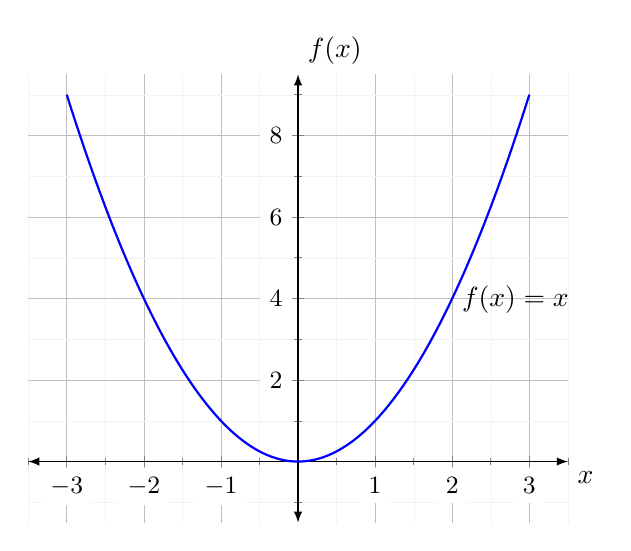
\begin{tikzpicture}
\begin{axis}[
    axis lines=middle,
    xlabel=\(x\),
    ylabel=\(f(x)\),
    xmin=-3, xmax=3,
    ymin=-1, ymax=9,
    grid=both,
    grid style={line width=.1pt, draw=gray!10},
    major grid style={line width=.2pt,draw=gray!50},
    minor tick num=1,
    enlargelimits={abs=0.5},
    axis line style={latex-latex},
    ticklabel style={font=\small,fill=white},
    xlabel style={at={(ticklabel* cs:1)},anchor=north west},
    ylabel style={at={(ticklabel* cs:1)},anchor=south west}
]
\addplot[domain=-3:3, samples=100, smooth, thick, blue] {x^2};
\node[anchor=west] at (axis cs: 2,4) {\(f(x) = x^2\)};
\end{axis}
\end{tikzpicture}

\begin{example}
Consider the function \( g(x) = \sin(x) \), which maps real numbers to their sine values.
\end{example}

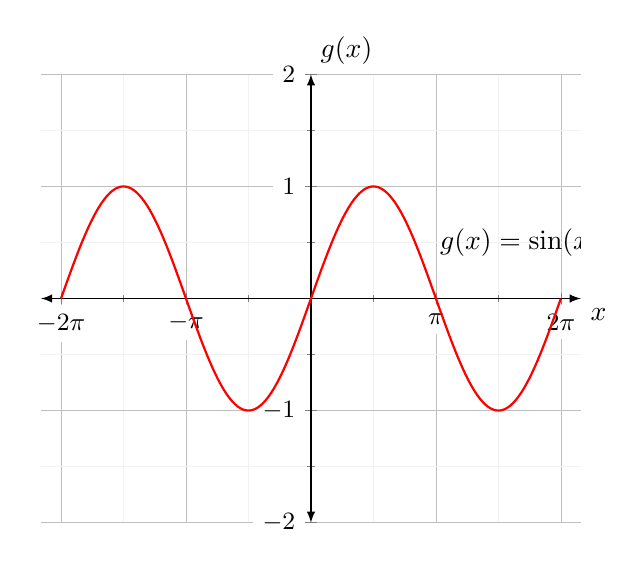
\begin{tikzpicture}
\begin{axis}[
    axis lines=middle,
    xlabel=\(x\),
    ylabel=\(g(x)\),
    xmin=-2*pi, xmax=2*pi,
    ymin=-1.5, ymax=1.5,
    grid=both,
    grid style={line width=.1pt, draw=gray!10},
    major grid style={line width=.2pt,draw=gray!50},
    minor tick num=1,
    enlargelimits={abs=0.5},
    axis line style={latex-latex},
    ticklabel style={font=\small,fill=white},
    xlabel style={at={(ticklabel* cs:1)},anchor=north west},
    ylabel style={at={(ticklabel* cs:1)},anchor=south west},
    xtick={-6.28318, -3.14159, 0, 3.14159, 6.28318},
    xticklabels={\(-2\pi\), \(-\pi\), 0, \(\pi\), \(2\pi\)}
]
\addplot[domain=-2*pi:2*pi, samples=100, smooth, thick, red] {sin(deg(x))};
\node[anchor=west] at (axis cs: 3,0.5) {\(g(x) = \sin(x)\)};
\end{axis}
\end{tikzpicture}

\begin{example}
Consider the piecewise function \( h(x) \) defined as \( h(x) = \left\{\begin{array}{ll} x^2 & \text{if } x \leq 0 \\ \sqrt{x} & \text{if } x > 0 \end{array}\right. \).
\end{example}

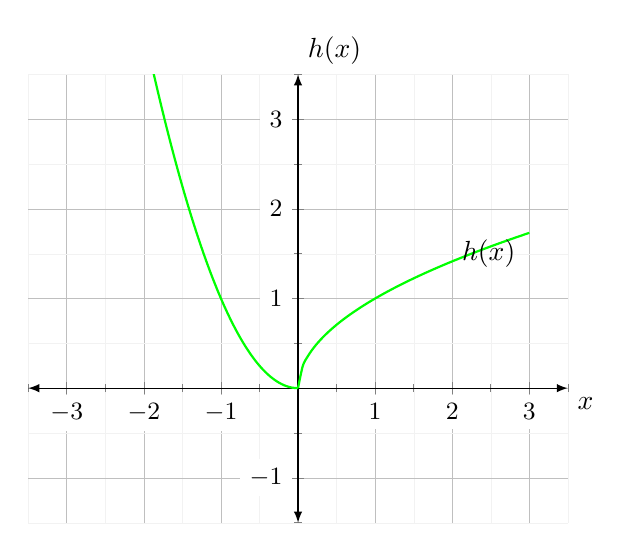
\begin{tikzpicture}
\begin{axis}[
    axis lines=middle,
    xlabel=\(x\),
    ylabel=\(h(x)\),
    xmin=-3, xmax=3,
    ymin=-1, ymax=3,
    grid=both,
    grid style={line width=.1pt, draw=gray!10},
    major grid style={line width=.2pt,draw=gray!50},
    minor tick num=1,
    enlargelimits={abs=0.5},
    axis line style={latex-latex},
    ticklabel style={font=\small,fill=white},
    xlabel style={at={(ticklabel* cs:1)},anchor=north west},
    ylabel style={at={(ticklabel* cs:1)},anchor=south west}
]
\addplot[domain=-3:0, samples=50, smooth, thick, green] {x^2};
\addplot[domain=0:3, samples=50, smooth, thick, green] {sqrt(x)};
\node[anchor=west] at (axis cs: 2,1.5) {\(h(x)\)};
\end{axis}
\end{tikzpicture}

\subsection{Exercises}
\begin{exercise}
Graph the function \( f(x) = 3x - 2 \). Identify its slope and y-intercept.
\end{exercise}

\begin{exercise}
Consider the function \( g(x) = \frac{1}{x} \). For what values of \( x \) is \( g(x) \) undefined?
\end{exercise}

\begin{exercise}
Find the domain and range of the function \( h(x) = \sqrt{x + 4} \).
\end{exercise}

\begin{exercise}
Determine if the function \( f(x) = x^3 - x \) is even, odd, or neither. Justify your answer.
\end{exercise}

\begin{exercise}
Sketch the graph of the piecewise function \( p(x) = \left\{\begin{array}{ll} x^2 & \text{if } x < 0 \\ x + 1 & \text{if } x \geq 0 \end{array}\right. \). Indicate any points of discontinuity.
\end{exercise}

\begin{exercise}
Given the function \( f(x) = 2x^2 - 5x + 3 \), find \( f(-1) \) and \( f(2) \).
\end{exercise}

\begin{exercise}
For the function \( f(x) = |x - 3| \), find the x-coordinate where \( f(x) = 0 \).
\end{exercise}

\begin{exercise}
Create a function \( f(x) \) that has a domain of all real numbers except \( x = 2 \) and a range of \( y \geq 0 \).
\end{exercise}

\begin{exercise}
Determine the intervals on which the function \( f(x) = -x^2 + 4x - 3 \) is increasing and decreasing.
\end{exercise}

\begin{exercise}
For the function \( g(x) = \cos(x) \), evaluate \( g(\pi/2) \) and \( g(\pi) \).
\end{exercise}

% You can add instructions for submitting solutions or further exploration activities here

\subsection{Solutions to Exercises}

\begin{solution}[1]
To graph \( f(x) = 3x - 2 \), we note that the slope (m) is 3 and the y-intercept (b) is -2. The graph is a straight line with these characteristics.

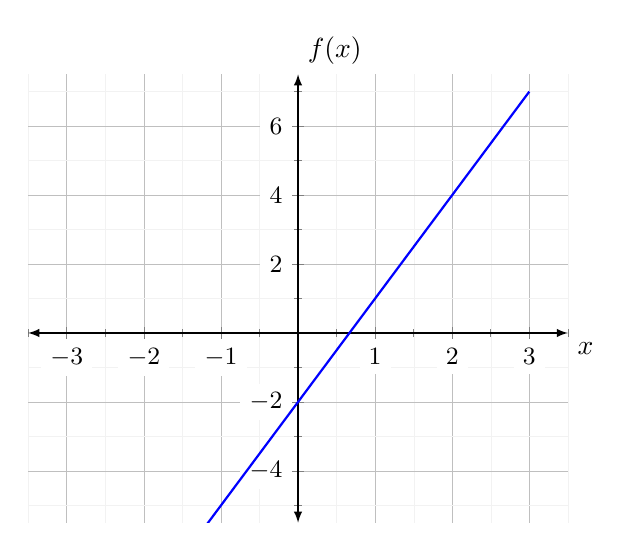
\begin{tikzpicture}
\begin{axis}[
    axis lines=middle,
    xlabel=\(x\),
    ylabel=\(f(x)\),
    xmin=-3, xmax=3,
    ymin=-5, ymax=7,
    grid=both,
    grid style={line width=.1pt, draw=gray!10},
    major grid style={line width=.2pt,draw=gray!50},
    minor tick num=1,
    enlargelimits={abs=0.5},
    axis line style={latex-latex},
    ticklabel style={font=\small,fill=white},
    xlabel style={at={(ticklabel* cs:1)},anchor=north west},
    ylabel style={at={(ticklabel* cs:1)},anchor=south west}
]
\addplot[domain=-3:3, samples=100, smooth, thick, blue] {3*x - 2};
\end{axis}
\end{tikzpicture}
\end{solution}

\begin{solution}[2]
The function \( g(x) = \frac{1}{x} \) is undefined when \( x = 0 \) because division by zero is not allowed.
\end{solution}

\begin{solution}[3]
For \( h(x) = \sqrt{x + 4} \), the domain is \( x \geq -4 \) (since the expression inside the square root must be non-negative), and the range is \( y \geq 0 \) (since the square root produces non-negative results).
\end{solution}

\begin{solution}[4]
The function \( f(x) = x^3 - x \) is odd because \( f(-x) = (-x)^3 - (-x) = -x^3 + x = -f(x) \).
\end{solution}

\begin{solution}[5]
The piecewise function \( p(x) \) is sketched below. It is discontinuous at \( x = 0 \) since the left-hand limit (0) does not equal the right-hand limit (1).

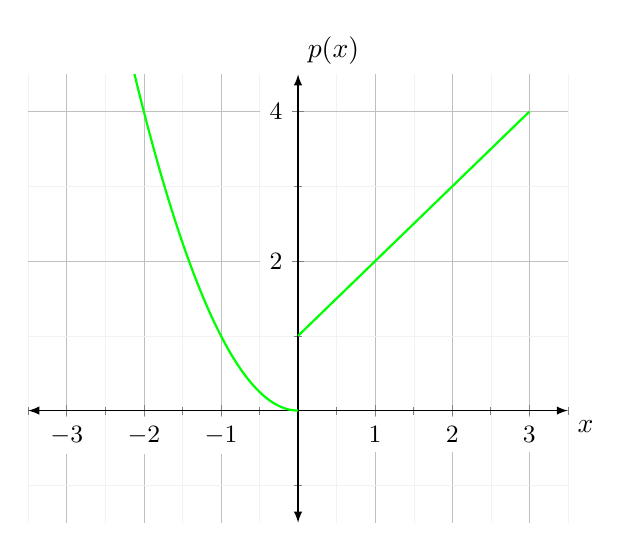
\begin{tikzpicture}
\begin{axis}[
    axis lines=middle,
    xlabel=\(x\),
    ylabel=\(p(x)\),
    xmin=-3, xmax=3,
    ymin=-1, ymax=4,
    grid=both,
    grid style={line width=.1pt, draw=gray!10},
    major grid style={line width=.2pt,draw=gray!50},
    minor tick num=1,
    enlargelimits={abs=0.5},
    axis line style={latex-latex},
    ticklabel style={font=\small,fill=white},
    xlabel style={at={(ticklabel* cs:1)},anchor=north west},
    ylabel style={at={(ticklabel* cs:1)},anchor=south west}
]
\addplot[domain=-3:0, samples=50, smooth, thick, green, unbounded coords=jump] {x^2};
\addplot[domain=0:3, samples=50, smooth, thick, green] {x + 1};
\end{axis}
\end{tikzpicture}
\end{solution}

\begin{solution}[6]
For \( f(x) = 2x^2 - 5x + 3 \), we find \( f(-1) = 2(-1)^2 - 5(-1) + 3 = 10 \) and \( f(2) = 2(2)^2 - 5(2) + 3 = -1 \).
\end{solution}

\begin{solution}[7]
The function \( f(x) = |x - 3| \) equals 0 when \( x - 3 = 0 \), i.e., \( x = 3 \).
\end{solution}

\begin{solution}[8]
One such function is \( f(x) = \frac{1}{(x-2)^2} \). The denominator ensures that \( x \neq 2 \) (domain), and the square ensures all output values are positive (range).
\end{solution}

\begin{solution}[9]
For \( f(x) = -x^2 + 4x - 3 \), the function is increasing where its derivative \( f'(x) = -2x + 4 \) is positive, i.e., for \( x < 2 \), and decreasing where \( f'(x) \) is negative, i.e., for \( x > 2 \).
\end{solution}

\begin{solution}[10]
For \( g(x) = \cos(x) \), we have \( g(\pi/2) = \cos(\pi/2) = 0 \) and \( g(\pi) = \cos(\pi) = -1 \).
\end{solution}

\section{Domain and Range}
\begin{definition}
The domain of a function is the set of all possible inputs, while the range is the set of all possible outputs.
\end{definition}

\begin{example}
For \( f(x) = \sqrt{x} \), the domain is \( x \geq 0 \) and the range is \( y \geq 0 \). The graph of this function is as follows:

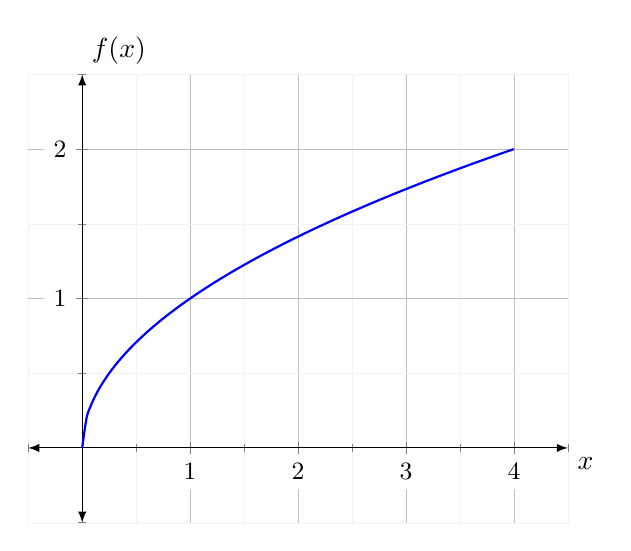
\begin{tikzpicture}
\begin{axis}[
    axis lines=middle,
    xlabel=\(x\),
    ylabel=\(f(x)\),
    xmin=0, xmax=4,
    ymin=0, ymax=2,
    samples=100,
    grid=both,
    grid style={line width=.1pt, draw=gray!10},
    major grid style={line width=.2pt,draw=gray!50},
    minor tick num=1,
    enlargelimits={abs=0.5},
    axis line style={latex-latex},
    ticklabel style={font=\small,fill=white},
    xlabel style={at={(ticklabel* cs:1)},anchor=north west},
    ylabel style={at={(ticklabel* cs:1)},anchor=south west}
]
\addplot[domain=0:4, smooth, thick, blue] {sqrt(x)};
\end{axis}
\end{tikzpicture}
\end{example}

\begin{example}
Consider the function \( g(x) = \frac{1}{x} \). Its domain is \( x \neq 0 \) and its range is \( y \neq 0 \). The graph is given by:

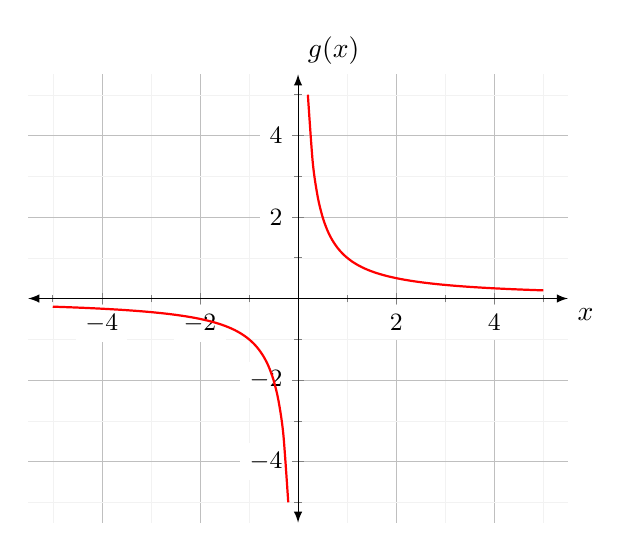
\begin{tikzpicture}
\begin{axis}[
    axis lines=middle,
    xlabel=\(x\),
    ylabel=\(g(x)\),
    xmin=-5, xmax=5,
    ymin=-5, ymax=5,
    samples=100,
    restrict y to domain=-5:5,
    grid=both,
    grid style={line width=.1pt, draw=gray!10},
    major grid style={line width=.2pt,draw=gray!50},
    minor tick num=1,
    enlargelimits={abs=0.5},
    axis line style={latex-latex},
    ticklabel style={font=\small,fill=white},
    xlabel style={at={(ticklabel* cs:1)},anchor=north west},
    ylabel style={at={(ticklabel* cs:1)},anchor=south west}
]
\addplot[domain=-5:-0.1, samples=50, smooth, thick, red] {1/x};
\addplot[domain=0.1:5, samples=50, smooth, thick, red] {1/x};
\end{axis}
\end{tikzpicture}
\end{example}

\begin{example}
For the function \( h(x) = x^2 - 4 \), the domain is all real numbers, but the range is \( y \geq -4 \). Its graph is:

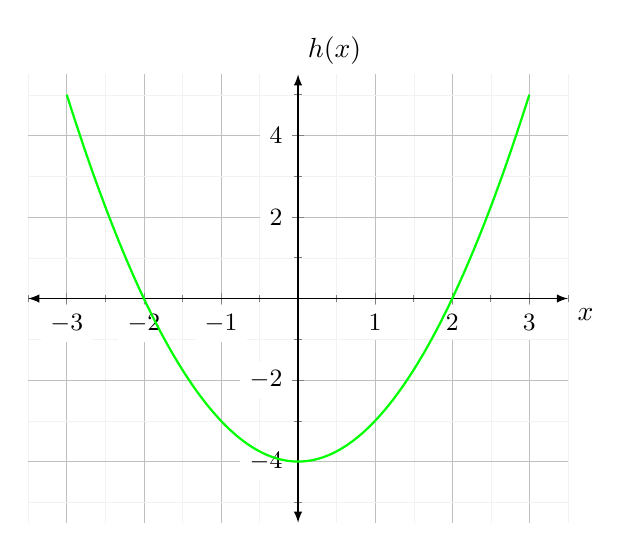
\begin{tikzpicture}
\begin{axis}[
    axis lines=middle,
    xlabel=\(x\),
    ylabel=\(h(x)\),
    xmin=-3, xmax=3,
    ymin=-5, ymax=5,
    samples=100,
    grid=both,
    grid style={line width=.1pt, draw=gray!10},
    major grid style={line width=.2pt,draw=gray!50},
    minor tick num=1,
    enlargelimits={abs=0.5},
    axis line style={latex-latex},
    ticklabel style={font=\small,fill=white},
    xlabel style={at={(ticklabel* cs:1)},anchor=north west},
    ylabel style={at={(ticklabel* cs:1)},anchor=south west}
]
\addplot[domain=-3:3, smooth, thick, green] {x^2 - 4};
\end{axis}
\end{tikzpicture}
\end{example}


\subsection{Exercises on Domain and Range}

\begin{exercise}
Determine the domain and range of the function \( f(x) = 2x + 3 \).
\end{exercise}

\begin{exercise}
Find the domain and range of the function \( g(x) = \frac{1}{x - 2} \).
\end{exercise}

\begin{exercise}
Identify the domain and range for the quadratic function \( h(x) = x^2 - 6x + 9 \).
\end{exercise}

\begin{exercise}
For the function \( k(x) = \ln(x - 1) \), determine its domain and range.
\end{exercise}

\begin{exercise}
Consider the function \( m(x) = \frac{x}{x^2 - 4} \). What are its domain and range?
\end{exercise}

\begin{exercise}
Find the domain and range for the trigonometric function \( n(x) = \sin(x) \).
\end{exercise}

\begin{exercise}
Determine the domain and range of the absolute value function \( p(x) = |x + 5| \).
\end{exercise}

\begin{exercise}
For the piecewise function \( q(x) = \begin{cases} x^2 & \text{if } x \leq 0 \\ 2x + 3 & \text{if } x > 0 \end{cases} \), identify the domain and range.
\end{exercise}

\begin{exercise}
Consider the exponential function \( r(x) = 2^x \). What is its domain and range?
\end{exercise}

\begin{exercise}
Identify the domain and range for the cubic function \( s(x) = x^3 - 3x \).
\end{exercise}

\subsection{Solutions to Exercises on Domain and Range}

\begin{solution}[1]
For \( f(x) = 2x + 3 \), the domain is all real numbers since there are no restrictions on \( x \). The range is also all real numbers because as \( x \) takes any real value, \( 2x + 3 \) also covers all real numbers.
\end{solution}

\begin{solution}[2]
The function \( g(x) = \frac{1}{x - 2} \) is undefined when \( x = 2 \), so the domain is \( x \neq 2 \). The range is all real numbers except \( y \neq 0 \) because the function never touches the y-axis.
\end{solution}

\begin{solution}[3]
For the quadratic function \( h(x) = x^2 - 6x + 9 \), the domain is all real numbers. Since the vertex of this parabola is at \( x = 3 \) and it opens upwards, the minimum value is \( h(3) = 0 \), thus the range is \( y \geq 0 \).
\end{solution}

\begin{solution}[4]
The function \( k(x) = \ln(x - 1) \) requires \( x - 1 > 0 \), so the domain is \( x > 1 \). The range of a natural logarithm function is all real numbers.
\end{solution}

\begin{solution}[5]
For \( m(x) = \frac{x}{x^2 - 4} \), the function is undefined for \( x = \pm 2 \), so the domain is \( x \neq \pm 2 \). The range is all real numbers, as the function can take any y-value.
\end{solution}

\begin{solution}[6]
The domain of the trigonometric function \( n(x) = \sin(x) \) is all real numbers. The range of the sine function is between -1 and 1, inclusive, so \( y \in [-1, 1] \).
\end{solution}

\begin{solution}[7]
For the absolute value function \( p(x) = |x + 5| \), the domain is all real numbers. The range is \( y \geq 0 \) since absolute values are always non-negative.
\end{solution}

\begin{solution}[8]
The piecewise function \( q(x) \) is defined for all real numbers, so the domain is all real numbers. To find the range, consider each piece: \( x^2 \) and \( 2x + 3 \). The range is all non-negative values for \( x^2 \) and all real numbers for \( 2x + 3 \), thus the range is all real numbers.
\end{solution}

\begin{solution}[9]
For the exponential function \( r(x) = 2^x \), the domain is all real numbers, as exponents can take any real value. The range is \( y > 0 \) since exponential functions are always positive.
\end{solution}

\begin{solution}[10]
The cubic function \( s(x) = x^3 - 3x \) has a domain of all real numbers. The range is also all real numbers because as a cubic function, it extends infinitely in both the positive and negative y-directions.
\end{solution}


\section{Types of Functions}
\subsection{Linear Functions}
\begin{definition}
A linear function has the form \( f(x) = mx + b \), where \( m \) is the slope of the line and \( b \) is the y-intercept.
\end{definition}

Linear functions are fundamental in calculus and represent the simplest form of polynomial functions. Their graph is a straight line, and they have constant rates of change.

\paragraph{Properties of Linear Functions:}
\begin{itemize}
    \item The slope \( m \) determines the steepness of the line and its direction (increasing or decreasing).
    \item The y-intercept \( b \) is the point where the line crosses the y-axis.
    \item Linear functions have a constant rate of change, which is equal to the slope \( m \).
\end{itemize}

\paragraph{Graphing a Linear Function:}
Consider the function \( f(x) = 2x + 3 \). Here, \( m = 2 \) and \( b = 3 \). The graph can be plotted as follows:

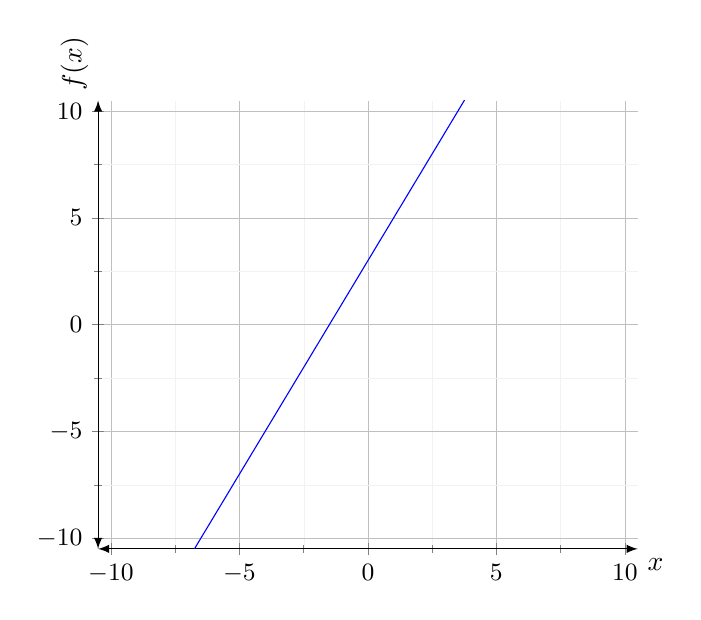
\begin{tikzpicture}
\begin{axis}[
    axis lines = left,
    xlabel = \( x \),
    ylabel = {\( f(x) \)},
    xmin=-10, xmax=10,
    ymin=-10, ymax=10,
    grid=both,
    grid style={line width=.1pt, draw=gray!10},
    major grid style={line width=.2pt,draw=gray!50},
    minor tick num=1,
    enlargelimits={abs=0.5},
    axis line style={latex-latex},
    ticklabel style={font=\small,fill=white},
    xlabel style={at={(ticklabel* cs:1)},anchor=north west},
    ylabel style={at={(ticklabel* cs:1)},anchor=south west}
]
% Plotting the line
\addplot[domain=-10:10, samples=100, color=blue]{2*x + 3};
\node[anchor=west] at (axis cs: 5,13) {\(f(x) = 2x + 3\)};
\end{axis}
\end{tikzpicture}

This line intersects the y-axis at (0, 3) and has a slope of 2, indicating it rises 2 units for every 1 unit it moves to the right.

\paragraph{Slope-Intercept Form:}
The equation \( f(x) = mx + b \) is known as the slope-intercept form of a linear function, where the slope \( m \) and y-intercept \( b \) are easily identifiable.

\paragraph{Applications of Linear Functions:}
Linear functions model relationships with a constant rate of change and are widely used in various fields such as economics, physics, and social sciences.

\begin{exercise}
Find the slope and y-intercept of the linear function \( g(x) = -3x + 7 \) and sketch its graph.
\end{exercise}

\begin{exercise}
If a linear function passes through the points (1, 2) and (3, 6), determine its equation.
\end{exercise}


\subsubsection*{Exercises on Linear Functions}

\begin{exercise}
Find the slope and y-intercept of the linear function \( g(x) = -3x + 7 \) and sketch its graph.
\end{exercise}

\begin{exercise}
If a linear function passes through the points (1, 2) and (3, 6), determine its equation.
\end{exercise}

\begin{exercise}
Determine the equation of the line that is parallel to \( f(x) = 4x - 5 \) and passes through the point (2, 3).
\end{exercise}

\begin{exercise}
Find the point of intersection of the linear functions \( f(x) = 2x + 1 \) and \( g(x) = -x + 5 \).
\end{exercise}

\begin{exercise}
A rental car company charges a base fee of \$50 and an additional \$20 per day. Write a linear function representing the total cost \( C \) as a function of the number of days \( d \) rented.
\end{exercise}

\begin{exercise}
Graph the linear function \( h(x) = -\frac{1}{2}x + 4 \) and identify where it intersects the x-axis and y-axis.
\end{exercise}

\begin{exercise}
A phone company offers a monthly plan for \$30 with an additional charge of \$0.05 per minute of calls. Write a linear function representing the monthly cost \( M \) as a function of the number of minutes \( m \) used.
\end{exercise}

\begin{exercise}
Determine whether the points (2, 4), (3, 6), and (5, 10) lie on the same linear function. If so, find the equation of the line.
\end{exercise}

\begin{exercise}
Find the slope of the line that passes through the points (-1, -2) and (3, 4).
\end{exercise}

\begin{exercise}
A company’s profit \( P \) in thousands of dollars is linearly related to the number of units \( n \) sold, with a profit of \$4,000 for 500 units and a loss of \$2,000 for 200 units. Determine the linear function that models the profit.
\end{exercise}

\subsubsection*{Solutions to Exercises on Linear Functions}

\begin{solution}[1]
For \( g(x) = -3x + 7 \), the slope (m) is -3, and the y-intercept (b) is 7. The graph is a straight line with a downward slope, crossing the y-axis at (0, 7).
\end{solution}

\begin{solution}[2]
To find the equation of a line passing through (1, 2) and (3, 6), calculate the slope \( m = \frac{6 - 2}{3 - 1} = 2 \). Using the point-slope form: \( y - 2 = 2(x - 1) \), the equation is \( y = 2x \).
\end{solution}

\begin{solution}[3]
A line parallel to \( f(x) = 4x - 5 \) has the same slope, m = 4. Passing through (2, 3), use point-slope form: \( y - 3 = 4(x - 2) \), yielding \( y = 4x - 5 \).
\end{solution}

\begin{solution}[4]
To find the intersection of \( f(x) = 2x + 1 \) and \( g(x) = -x + 5 \), set them equal: \( 2x + 1 = -x + 5 \). Solving gives \( x = \frac{4}{3} \), and substituting back, \( y = \frac{11}{3} \). Thus, they intersect at \( (\frac{4}{3}, \frac{11}{3}) \).
\end{solution}

\begin{solution}[5]
The total cost \( C \) is given by \( C = 50 + 20d \), where \( d \) is the number of days rented.
\end{solution}

\begin{solution}[6]
For \( h(x) = -\frac{1}{2}x + 4 \), the graph intersects the y-axis at (0, 4) and intersects the x-axis at \( x \) where \( h(x) = 0 \). Setting the equation to 0 gives \( x = 8 \). So, it intersects the x-axis at (8, 0).
\end{solution}

\begin{solution}[7]
The monthly cost \( M \) is \( M = 30 + 0.05m \), where \( m \) is the number of minutes used.
\end{solution}

\begin{solution}[8]
The slope between (2, 4) and (3, 6) is 2, and between (3, 6) and (5, 10) is also 2. Since the slope is consistent, they lie on the same line. The line equation, using point-slope form, is \( y = 2x \).
\end{solution}

\begin{solution}[9]
The slope is \( \frac{4 - (-2)}{3 - (-1)} = \frac{6}{4} = \frac{3}{2} \).
\end{solution}

\begin{solution}[10]
Let \( P = mn + b \). Using given points, form equations: \( 4000 = 500m + b \) and \( -2000 = 200m + b \). Solving these simultaneously gives \( m = 20 \) and \( b = -6000 \). So, \( P = 20n - 6000 \).
\end{solution}


\subsection{Polynomial Functions}
\begin{definition}
A polynomial function is of the form \( f(x) = a_nx^n + a_{n-1}x^{n-1} + \cdots + a_0 \), where \( n \) is a non-negative integer, and \( a_n, a_{n-1}, \ldots, a_0 \) are constants.
\end{definition}

Polynomial functions are fundamental in calculus and algebra. They can range from simple linear functions to complex equations with high degrees. The highest power of \( x \) in the function (the degree of the polynomial) greatly influences the shape and behavior of its graph.

\paragraph{Characteristics of Polynomial Functions:}
\begin{itemize}
    \item The degree of the polynomial determines its basic shape and the number of roots.
    \item Polynomials are continuous and smooth functions.
    \item The leading coefficient \( a_n \) affects the end behavior of the polynomial.
\end{itemize}

\paragraph{Graphing Polynomial Functions:}
Consider the quadratic function \( f(x) = x^2 - 4x + 3 \). Its graph can be plotted as follows:

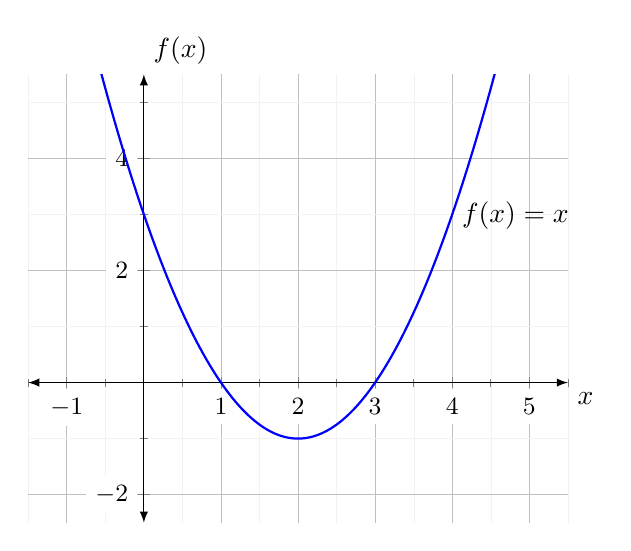
\begin{tikzpicture}
\begin{axis}[
    axis lines=middle,
    xlabel=\(x\),
    ylabel=\(f(x)\),
    xmin=-1, xmax=5,
    ymin=-2, ymax=5,
    samples=100,
    grid=both,
    grid style={line width=.1pt, draw=gray!10},
    major grid style={line width=.2pt,draw=gray!50},
    minor tick num=1,
    enlargelimits={abs=0.5},
    axis line style={latex-latex},
    ticklabel style={font=\small,fill=white},
    xlabel style={at={(ticklabel* cs:1)},anchor=north west},
    ylabel style={at={(ticklabel* cs:1)},anchor=south west}
]
% Plotting the polynomial
\addplot[domain=-1:5, smooth, thick, blue]{x^2 - 4*x + 3};
\node[anchor=west] at (axis cs: 4,3) {\(f(x) = x^2 - 4x + 3\)};
\end{axis}
\end{tikzpicture}

This graph represents a parabola opening upwards with its vertex and intercepts easily identifiable.

\paragraph{Real-World Applications:}
Polynomial functions model numerous real-world phenomena, including projectile motion, profit and loss calculations, population growth, and much more.

\begin{exercise}
Sketch the graph of the cubic function \( g(x) = x^3 - 6x^2 + 11x - 6 \). Identify its roots and turning points.
\end{exercise}

\begin{exercise}
Find a polynomial of degree 3 that has roots at \( x = 1, 2, \) and \( 3 \).
\end{exercise}

\subsubsection*{Exercises on Polynomial Functions}

\begin{exercise}
Sketch the graph of the cubic function \( g(x) = x^3 - 6x^2 + 11x - 6 \). Identify its roots and turning points.
\end{exercise}

\begin{exercise}
Find a polynomial of degree 3 that has roots at \( x = 1, 2, \) and \( 3 \).
\end{exercise}

\begin{exercise}
Determine the degree and leading coefficient of the polynomial \( h(x) = 4x^4 - 3x^3 + 2x^2 - x + 7 \).
\end{exercise}

\begin{exercise}
For the quadratic function \( f(x) = 2x^2 - 8x + 6 \), find the vertex and axis of symmetry. Also, determine whether it opens upwards or downwards.
\end{exercise}

\begin{exercise}
Write the polynomial function \( p(x) = x^3 - 4x \) in factored form and identify its zeros.
\end{exercise}

\begin{exercise}
A polynomial function has zeros at \( x = -2, 0, \) and \( 4 \) with a leading coefficient of 1. Write the equation of this polynomial.
\end{exercise}

\begin{exercise}
Given the polynomial \( q(x) = x^4 - 10x^2 + 9 \), find the y-intercept and x-intercepts (if any).
\end{exercise}

\begin{exercise}
Graph the polynomial \( r(x) = -x^3 + 3x^2 - 2x \) and determine the intervals where the function is increasing and decreasing.
\end{exercise}

\begin{exercise}
For the polynomial function \( s(x) = 3x^3 - 5x^2 + x - 2 \), use synthetic division to determine whether \( x = 1 \) is a zero of \( s \).
\end{exercise}

\begin{exercise}
Consider the polynomial \( t(x) = x^4 - 2x^2 - 3 \). Find all the real zeros of \( t \) and sketch the graph of the function.
\end{exercise}

\subsubsection*{Solutions to Exercises on Polynomial Functions}

\begin{solution}[1]
For \( g(x) = x^3 - 6x^2 + 11x - 6 \), the roots are found by solving \( g(x) = 0 \). The roots are \( x = 1, 2, 3 \). Turning points occur where the derivative changes sign. Calculating \( g'(x) = 3x^2 - 12x + 11 \) and finding its roots gives the turning points at approximately \( x \approx 1.57 \) and \( x \approx 2.43 \).
\end{solution}

\begin{solution}[2]
A polynomial of degree 3 with roots at \( x = 1, 2, 3 \) can be written as \( f(x) = (x - 1)(x - 2)(x - 3) \).
\end{solution}

\begin{solution}[3]
The degree of the polynomial \( h(x) = 4x^4 - 3x^3 + 2x^2 - x + 7 \) is 4, and the leading coefficient is 4.
\end{solution}

\begin{solution}[4]
For \( f(x) = 2x^2 - 8x + 6 \), the vertex form is \( f(x) = 2(x - 2)^2 + 2 \). The vertex is at (2, 2), and the axis of symmetry is \( x = 2 \). The parabola opens upwards since the coefficient of \( x^2 \) is positive.
\end{solution}

\begin{solution}[5]
The polynomial \( p(x) = x^3 - 4x \) can be factored as \( p(x) = x(x^2 - 4) = x(x - 2)(x + 2) \). The zeros are at \( x = 0, 2, -2 \).
\end{solution}

\begin{solution}[6]
A polynomial with zeros at \( x = -2, 0, \) and \( 4 \) and a leading coefficient of 1 is \( f(x) = (x + 2)x(x - 4) = x^3 - 4x^2 - 2x \).
\end{solution}

\begin{solution}[7]
For \( q(x) = x^4 - 10x^2 + 9 \), the y-intercept is \( q(0) = 9 \). To find the x-intercepts, solve \( x^4 - 10x^2 + 9 = 0 \), which gives \( x \approx \pm 3.16, \pm 0.84 \).
\end{solution}

\begin{solution}[8]
Graphing \( r(x) = -x^3 + 3x^2 - 2x \), the function increases where \( r'(x) > 0 \) and decreases where \( r'(x) < 0 \). Calculating \( r'(x) = -3x^2 + 6x - 2 \) and finding its roots gives the intervals of increase and decrease.
\end{solution}

\begin{solution}[9]
Using synthetic division to divide \( 3x^3 - 5x^2 + x - 2 \) by \( x - 1 \), we find that the remainder is not zero. Hence, \( x = 1 \) is not a zero of \( s(x) \).
\end{solution}

\begin{solution}[10]
To find the real zeros of \( t(x) = x^4 - 2x^2 - 3 \), solve \( x^4 - 2x^2 - 3 = 0 \). The real zeros are approximately \( x \approx \pm 1.73, \pm 1.00 \). Graphing \( t(x) \) would show a polynomial crossing the x-axis at these points.
\end{solution}


\subsection{Rational Functions}
\begin{definition}
A rational function is the ratio of two polynomial functions, typically expressed in the form \( f(x) = \frac{p(x)}{q(x)} \), where both \( p(x) \) and \( q(x) \) are polynomial functions and \( q(x) \neq 0 \).
\end{definition}

Rational functions can exhibit a variety of behaviors, including asymptotes and discontinuities, making them interesting subjects of study in calculus.

\paragraph{Characteristics of Rational Functions:}
\begin{itemize}
    \item The vertical asymptotes occur at values of \( x \) for which \( q(x) = 0 \), provided these points are not cancelled out by the numerator.
    \item Horizontal asymptotes are determined by the degrees of \( p(x) \) and \( q(x) \).
    \item Rational functions may have holes if a factor in the denominator is cancelled out by the numerator.
\end{itemize}

\paragraph{Graphing Rational Functions:}
Consider the function \( f(x) = \frac{x^2 - 4}{x - 2} \). Here, we have a hole at \( x = 2 \) because the factor \( (x - 2) \) is cancelled. The graph can be plotted as follows:

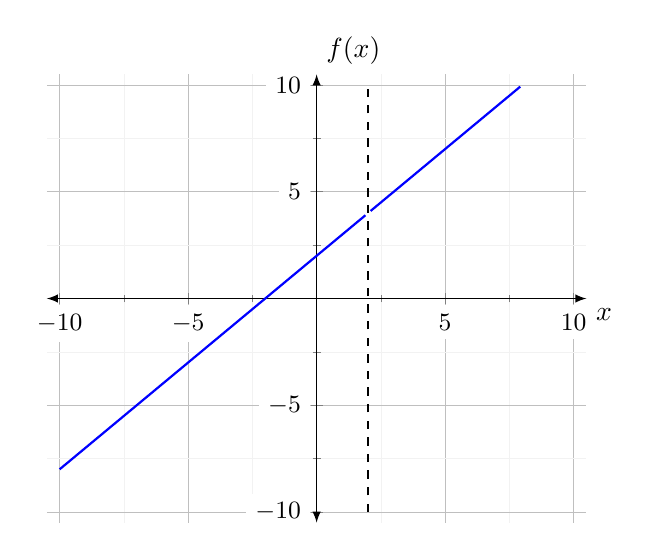
\begin{tikzpicture}
\begin{axis}[
    axis lines = middle,
    xlabel = \( x \),
    ylabel = {\( f(x) \)},
    xmin=-10, xmax=10,
    ymin=-10, ymax=10,
    restrict y to domain=-10:10,
    samples=100,
    grid=both,
    grid style={line width=.1pt, draw=gray!10},
    major grid style={line width=.2pt,draw=gray!50},
    minor tick num=1,
    enlargelimits={abs=0.5},
    axis line style={latex-latex},
    ticklabel style={font=\small,fill=white},
    xlabel style={at={(ticklabel* cs:1)},anchor=north west},
    ylabel style={at={(ticklabel* cs:1)},anchor=south west}
]
% Plotting the rational function
\addplot[domain=-10:1.9, smooth, thick, blue]{(x^2 - 4)/(x - 2)};
\addplot[domain=2.1:10, smooth, thick, blue]{(x^2 - 4)/(x - 2)};
\draw[dashed] (axis cs:2,-10) -- (axis cs:2,10);
\end{axis}
\end{tikzpicture}

\paragraph{Applications of Rational Functions:}
Rational functions are used in various fields, including engineering, economics, and physics, to model scenarios where variables inversely affect each other.

\begin{exercise}
Graph the rational function \( g(x) = \frac{1}{x - 1} \) and determine its vertical and horizontal asymptotes.
\end{exercise}

\begin{exercise}
Consider the function \( h(x) = \frac{x^2 - 1}{x^2 + x - 2} \). Identify its vertical and horizontal asymptotes, and sketch the graph.
\end{exercise}

\subsubsection*{Exercises on Rational Functions}

\begin{exercise}
Graph the rational function \( g(x) = \frac{1}{x - 1} \) and determine its vertical and horizontal asymptotes.
\end{exercise}

\begin{exercise}
Consider the function \( h(x) = \frac{x^2 - 1}{x^2 + x - 2} \). Identify its vertical and horizontal asymptotes, and sketch the graph.
\end{exercise}

\begin{exercise}
Find the domain of the rational function \( f(x) = \frac{2x - 3}{x^2 - 4} \).
\end{exercise}

\begin{exercise}
Determine the vertical and horizontal asymptotes for the function \( p(x) = \frac{x^3 - 4x}{x^2 - 5x + 6} \) and sketch its graph.
\end{exercise}

\begin{exercise}
For the rational function \( q(x) = \frac{x^2 + 2x + 1}{x^2 - 1} \), identify any holes or asymptotes, and graph the function.
\end{exercise}

\begin{exercise}
Given \( r(x) = \frac{3x - 5}{2x + 4} \), calculate \( r(2) \) and determine the behavior of \( r(x) \) as \( x \) approaches infinity.
\end{exercise}

\begin{exercise}
Sketch the graph of the function \( s(x) = \frac{x}{x^2 - 9} \) and find the x- and y-intercepts.
\end{exercise}

\begin{exercise}
Analyze the rational function \( t(x) = \frac{5x - 4}{x - 3} \) for any asymptotes or discontinuities and provide its graph.
\end{exercise}

\begin{exercise}
Find the range of the function \( u(x) = \frac{2}{x - 1} + 3 \).
\end{exercise}

\begin{exercise}
Determine the inverse of the function \( v(x) = \frac{1}{2 - x} \).
\end{exercise}

\subsubsection*{Solutions to Exercises on Rational Functions}

\begin{solution}[1]
For \( g(x) = \frac{1}{x - 1} \), the vertical asymptote is at \( x = 1 \) (where the denominator equals zero), and the horizontal asymptote is \( y = 0 \) (as \( x \) approaches infinity, \( g(x) \) approaches 0).
\end{solution}

\begin{solution}[2]
In \( h(x) = \frac{x^2 - 1}{x^2 + x - 2} \), the vertical asymptotes are at the roots of the denominator, \( x = 1 \) and \( x = -2 \). The horizontal asymptote is \( y = 1 \) as the degrees of the numerator and denominator are the same.
\end{solution}

\begin{solution}[3]
The domain of \( f(x) = \frac{2x - 3}{x^2 - 4} \) is all real numbers except \( x = \pm 2 \), where the denominator equals zero.
\end{solution}

\begin{solution}[4]
For \( p(x) = \frac{x^3 - 4x}{x^2 - 5x + 6} \), vertical asymptotes are at \( x = 2 \) and \( x = 3 \), the roots of the denominator. There is no horizontal asymptote as the degree of the numerator is greater than that of the denominator.
\end{solution}

\begin{solution}[5]
In \( q(x) = \frac{x^2 + 2x + 1}{x^2 - 1} \), there is a hole at \( x = -1 \) (factor cancelled in numerator and denominator), vertical asymptotes at \( x = \pm 1 \), and no horizontal asymptote.
\end{solution}

\begin{solution}[6]
For \( r(x) = \frac{3x - 5}{2x + 4} \), \( r(2) = \frac{1}{8} \). As \( x \) approaches infinity, \( r(x) \) approaches \( \frac{3}{2} \).
\end{solution}

\begin{solution}[7]
In \( s(x) = \frac{x}{x^2 - 9} \), the x-intercepts are at \( x = 0 \), y-intercept at \( y = 0 \), and vertical asymptotes at \( x = \pm 3 \).
\end{solution}

\begin{solution}[8]
The function \( t(x) = \frac{5x - 4}{x - 3} \) has a vertical asymptote at \( x = 3 \) and no horizontal asymptote. Discontinuity occurs at \( x = 3 \).
\end{solution}

\begin{solution}[9]
To find the range of \( u(x) = \frac{2}{x - 1} + 3 \), consider the behavior as \( x \) approaches 1 and infinity. The range is all real numbers except \( y = 3 \).
\end{solution}

\begin{solution}[10]
The inverse of \( v(x) = \frac{1}{2 - x} \) can be found by swapping \( x \) and \( y \) and solving for \( y \): \( x = \frac{1}{2 - y} \) leads to \( y = 2 - \frac{1}{x} \).
\end{solution}

\subsection{Trigonometric Functions}
\begin{definition}
Trigonometric functions include \( \sin(x) \), \( \cos(x) \), and \( \tan(x) \), relating angles to ratios of sides in right triangles.
\end{definition}

Trigonometric functions are fundamental in calculus, physics, and engineering. They are periodic functions and have various properties that are essential in the study of waves, oscillations, and circular motion.

\paragraph{Properties of Trigonometric Functions:}
\begin{itemize}
    \item The functions \( \sin(x) \) and \( \cos(x) \) are periodic with a period of \( 2\pi \).
    \item The function \( \tan(x) \) is periodic with a period of \( \pi \).
    \item These functions have specific symmetries: \( \sin(x) \) is odd, \( \cos(x) \) is even, and \( \tan(x) \) is odd.
\end{itemize}

\paragraph{Graphing Trigonometric Functions:}
Using `pgfplots` to graph \( \sin(x) \) and \( \cos(x) \):

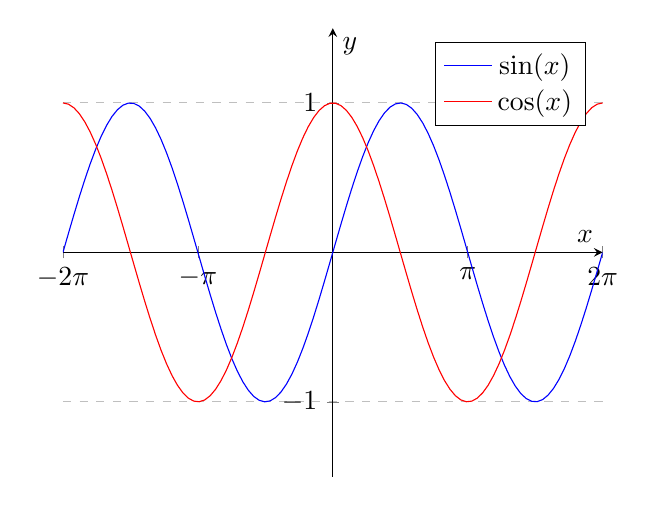
\begin{tikzpicture}
\begin{axis}[
    axis lines=middle,
    xlabel=\(x\),
    ylabel=\(y\),
    xmin=-2*pi, xmax=2*pi,
    ymin=-1.5, ymax=1.5,
    xtick={-6.28318, -3.14159, 0, 3.14159, 6.28318},
    xticklabels={\(-2\pi\), \(-\pi\), 0, \(\pi\), \(2\pi\)},
    ytick={-1, 0, 1},
    legend pos=north east,
    ymajorgrids=true,
    grid style=dashed,
]

% Plotting sin(x)
\addplot[domain=-2*pi:2*pi, samples=100, color=blue]{sin(deg(x))};
\addlegendentry{\(\sin(x)\)}

% Plotting cos(x)
\addplot[domain=-2*pi:2*pi, samples=100, color=red]{cos(deg(x))};
\addlegendentry{\(\cos(x)\)}
\end{axis}
\end{tikzpicture}

\paragraph{Applications of Trigonometric Functions:}
Trigonometric functions model phenomena such as sound waves, light waves, and describe the motion of pendulums and other periodic phenomena.

\begin{exercise}
Graph the function \( f(x) = \tan(x) \) and identify its asymptotes.
\end{exercise}

\begin{exercise}
Find the amplitude and period of the function \( g(x) = 3\sin(2x) \).
\end{exercise}

\begin{exercise}
Determine the phase shift and vertical shift for the function \( h(x) = \cos(x - \pi/2) + 1 \).
\end{exercise}

\subsubsection*{Exercises on Trigonometric Functions}

\begin{exercise}
Graph the function \( f(x) = \tan(x) \) and identify its asymptotes.
\end{exercise}

\begin{exercise}
Find the amplitude and period of the function \( g(x) = 3\sin(2x) \).
\end{exercise}

\begin{exercise}
Determine the phase shift and vertical shift for the function \( h(x) = \cos(x - \pi/2) + 1 \).
\end{exercise}

\begin{exercise}
Prove that \( \sin^2(x) + \cos^2(x) = 1 \) using a unit circle.
\end{exercise}

\begin{exercise}
Evaluate \( \sin(\pi/6) \), \( \cos(\pi/3) \), and \( \tan(\pi/4) \).
\end{exercise}

\begin{exercise}
Sketch the graph of \( f(x) = \sin(x) - \cos(x) \) over the interval \([0, 2\pi]\).
\end{exercise}

\begin{exercise}
Find the values of \( x \) where \( \sin(x) = -\sqrt{3}/2 \) in the interval \([-\pi, \pi]\).
\end{exercise}

\begin{exercise}
For the function \( g(x) = 2\cos(3x - \pi) \), identify the amplitude, period, phase shift, and sketch its graph.
\end{exercise}

\begin{exercise}
Determine the exact value of \( \tan(\pi/6) + \cos(\pi/3) \).
\end{exercise}

\begin{exercise}
Solve for \( x \) in the equation \( 3\sin(x) + 4\cos(x) = 0 \) over the interval \([0, 2\pi]\).
\end{exercise}

\subsubsection*{Solutions to Exercises on Trigonometric Functions}

\begin{solution}[1]
For \( f(x) = \tan(x) \), the graph has vertical asymptotes at \( x = \pm \frac{\pi}{2}, \pm \frac{3\pi}{2}, \ldots \) where the cosine function in the denominator equals zero.
\end{solution}

\begin{solution}[2]
The function \( g(x) = 3\sin(2x) \) has an amplitude of 3 (the coefficient of the sine function) and a period of \( \frac{\pi}{2} \) (computed as \( \frac{2\pi}{2} = \pi \)).
\end{solution}

\begin{solution}[3]
For \( h(x) = \cos(x - \pi/2) + 1 \), the phase shift is \( \frac{\pi}{2} \) to the right, and the vertical shift is 1 unit upwards.
\end{solution}

\begin{solution}[4]
Using the unit circle, we know that \( \sin(x) \) and \( \cos(x) \) represent the y-coordinate and x-coordinate, respectively, of a point on the circle. Since the radius of the unit circle is 1, we have \( \sin^2(x) + \cos^2(x) = 1^2 = 1 \).
\end{solution}

\begin{solution}[5]
Evaluate \( \sin(\pi/6) = 1/2 \), \( \cos(\pi/3) = 1/2 \), and \( \tan(\pi/4) = 1 \).
\end{solution}

\begin{solution}[6]
To graph \( f(x) = \sin(x) - \cos(x) \), plot the sine and cosine functions separately and then subtract their values for each \( x \) in the interval \([0, 2\pi]\).
\end{solution}

\begin{solution}[7]
The values of \( x \) where \( \sin(x) = -\sqrt{3}/2 \) in the interval \([-\pi, \pi]\) are \( x = -\pi/3 \) and \( x = -2\pi/3 \).
\end{solution}

\begin{solution}[8]
For \( g(x) = 2\cos(3x - \pi) \), the amplitude is 2, the period is \( \frac{2\pi}{3} \), and the phase shift is \( \frac{\pi}{3} \) to the right. Sketch the graph accordingly.
\end{solution}

\begin{solution}[9]
The exact value of \( \tan(\pi/6) + \cos(\pi/3) \) is \( \frac{\sqrt{3}}{3} + \frac{1}{2} \).
\end{solution}

\begin{solution}[10]
Solve \( 3\sin(x) + 4\cos(x) = 0 \) over the interval \([0, 2\pi]\). Dividing by \( \cos(x) \) and applying trigonometric identities, we find \( x = \frac{\pi}{2}, \frac{3\pi}{2} \).
\end{solution}

\subsection{Exponential and Logarithmic Functions}
\begin{definition}
Exponential functions have the form \( f(x) = a^x \) where \( a \) is a positive constant. Logarithmic functions are the inverses of exponential functions and are usually expressed as \( g(x) = \log_a(x) \) for a logarithm to the base \( a \).
\end{definition}

Exponential and logarithmic functions are widely used in many fields, including physics, engineering, and economics, due to their properties of describing growth and decay processes.

\paragraph{Characteristics of Exponential Functions:}
\begin{itemize}
    \item Exponential growth occurs when \( a > 1 \), and exponential decay happens when \( 0 < a < 1 \).
    \item The graph of an exponential function always lies above the x-axis and increases or decreases rapidly.
    \item Exponential functions have a horizontal asymptote at \( y = 0 \).
\end{itemize}

\paragraph{Characteristics of Logarithmic Functions:}
\begin{itemize}
    \item The logarithmic function \( \log_a(x) \) is undefined for \( x \leq 0 \).
    \item The graph of a logarithmic function passes through the point \( (1, 0) \) and has a vertical asymptote at \( x = 0 \).
    \item Logarithmic functions increase slowly and are used to model the inverse of exponential growth or decay.
\end{itemize}

\paragraph{Graphing Exponential and Logarithmic Functions:}
Here we graph \( f(x) = 2^x \) and its inverse \( g(x) = \log_2(x) \) using `pgfplots`:

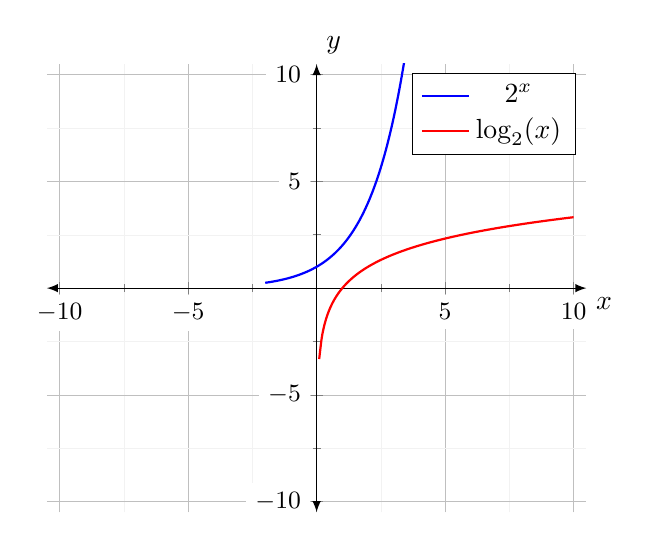
\begin{tikzpicture}
\begin{axis}[
    axis lines = middle,
    xlabel = \( x \),
    ylabel = {\( y \)},
    xmin=-10, xmax=10,
    ymin=-10, ymax=10,
    samples=100,
    grid=both,
    grid style={line width=.1pt, draw=gray!10},
    major grid style={line width=.2pt,draw=gray!50},
    minor tick num=1,
    enlargelimits={abs=0.5},
    axis line style={latex-latex},
    ticklabel style={font=\small,fill=white},
    xlabel style={at={(ticklabel* cs:1)},anchor=north west},
    ylabel style={at={(ticklabel* cs:1)},anchor=south west}
]

% Plotting the exponential function
\addplot[domain=-2:3.5, smooth, thick, blue]{2^x};
\addlegendentry{\(2^x\)}

% Plotting the logarithmic function
\addplot[domain=0.1:10, smooth, thick, red]{log2(x)};
\addlegendentry{\(\log_2(x)\)}
\end{axis}
\end{tikzpicture}

\begin{exercise}
Graph the exponential function \( h(x) = e^x \) and identify its key characteristics.
\end{exercise}

\begin{exercise}
Sketch the graph of \( k(x) = \log_e(x) \) (also known as \( \ln(x) \)) and discuss its properties.
\end{exercise}

\subsubsection*{Exercises on Exponential and Logarithmic Functions}

\begin{exercise}
Graph the exponential function \( h(x) = e^x \) and identify its key characteristics.
\end{exercise}

\begin{exercise}
Sketch the graph of \( k(x) = \log_e(x) \) (also known as \( \ln(x) \)) and discuss its properties.
\end{exercise}

\begin{exercise}
Evaluate the expression \( e^{\ln(5)} \) and explain the relationship between the exponential and logarithmic functions.
\end{exercise}

\begin{exercise}
Find the solution to the equation \( 3^x = 27 \).
\end{exercise}

\begin{exercise}
Determine the x-intercept of the logarithmic function \( f(x) = \log_2(x - 1) \).
\end{exercise}

\begin{exercise}
Solve for \( x \) in the equation \( \ln(x) + \ln(2x) = 3 \).
\end{exercise}

\begin{exercise}
Graph the function \( g(x) = 2^x + 3 \) and describe how it differs from the basic exponential function \( f(x) = 2^x \).
\end{exercise}

\begin{exercise}
Find the domain and range of the function \( h(x) = \ln(x - 2) \).
\end{exercise}

\begin{exercise}
Calculate the derivative of the function \( f(x) = e^{2x} \) using the rules of differentiation for exponential functions.
\end{exercise}

\begin{exercise}
Given the function \( g(x) = \log_{10}(x^2 - 1) \), find the points of discontinuity.
\end{exercise}

\subsubsection*{Solutions to Exercises on Exponential and Logarithmic Functions}

\begin{solution}[1]
For \( h(x) = e^x \), the graph is an increasing exponential function. It passes through the point (0, 1) and has a horizontal asymptote at \( y = 0 \). The function is always positive and increases rapidly as \( x \) increases.
\end{solution}

\begin{solution}[2]
The function \( k(x) = \log_e(x) \), or \( \ln(x) \), has a graph that passes through the point (1, 0) and has a vertical asymptote at \( x = 0 \). The function is defined for \( x > 0 \) and increases slowly as \( x \) increases.
\end{solution}

\begin{solution}[3]
Evaluate \( e^{\ln(5)} \). Since the exponential and logarithmic functions are inverses of each other, \( e^{\ln(5)} = 5 \).
\end{solution}

\begin{solution}[4]
Solve \( 3^x = 27 \). Recognizing that \( 27 = 3^3 \), we find \( x = 3 \).
\end{solution}

\begin{solution}[5]
To find the x-intercept of \( f(x) = \log_2(x - 1) \), set \( f(x) = 0 \). This yields \( \log_2(x - 1) = 0 \), so \( x - 1 = 1 \), and thus \( x = 2 \).
\end{solution}

\begin{solution}[6]
Solve \( \ln(x) + \ln(2x) = 3 \). Combine the logarithms: \( \ln(2x^2) = 3 \). Exponentiating both sides gives \( 2x^2 = e^3 \). Solving for \( x \) yields \( x = \pm \sqrt{\frac{e^3}{2}} \), but only the positive solution is valid since \( \ln(x) \) is undefined for negative \( x \).
\end{solution}

\begin{solution}[7]
Graph \( g(x) = 2^x + 3 \). This graph is a vertical shift of the function \( f(x) = 2^x \) upwards by 3 units. It increases exponentially and passes through the point (0, 4).
\end{solution}

\begin{solution}[8]
The domain of \( h(x) = \ln(x - 2) \) is \( x > 2 \), and the range is all real numbers since the logarithmic function can take any real value.
\end{solution}

\begin{solution}[9]
The derivative of \( f(x) = e^{2x} \) is \( f'(x) = 2e^{2x} \), using the chain rule for differentiation.
\end{solution}

\begin{solution}[10]
For \( g(x) = \log_{10}(x^2 - 1) \), the function is undefined at points where \( x^2 - 1 \leq 0 \), which occurs at \( x = -1 \) and \( x = 1 \). These are the points of discontinuity.
\end{solution}


\section{Function Properties}
\subsection{Continuity}
\begin{definition}
A function is continuous at a point if the limit of the function as it approaches the point is equal to the function value at that point. Formally, a function \( f(x) \) is continuous at a point \( c \) if \( \lim_{x \to c} f(x) = f(c) \).
\end{definition}

Continuity is a fundamental concept in calculus, essential for understanding limits, derivatives, and integrals.

\paragraph{Types of Discontinuities:}
\begin{itemize}
    \item A function has a \textit{removable discontinuity} at a point if the limit exists but is not equal to the function value at that point.
    \item A \textit{jump discontinuity} occurs when the left-hand and right-hand limits exist but are not equal to each other.
    \item An \textit{infinite discontinuity} occurs when the function approaches infinity near the point of discontinuity.
\end{itemize}

\paragraph{Graphing Continuous Functions:}
To illustrate continuity, consider the function \( f(x) = \frac{x^2 - 4}{x - 2} \) and its simplified form \( g(x) = x + 2 \). The function \( f(x) \) has a removable discontinuity at \( x = 2 \).

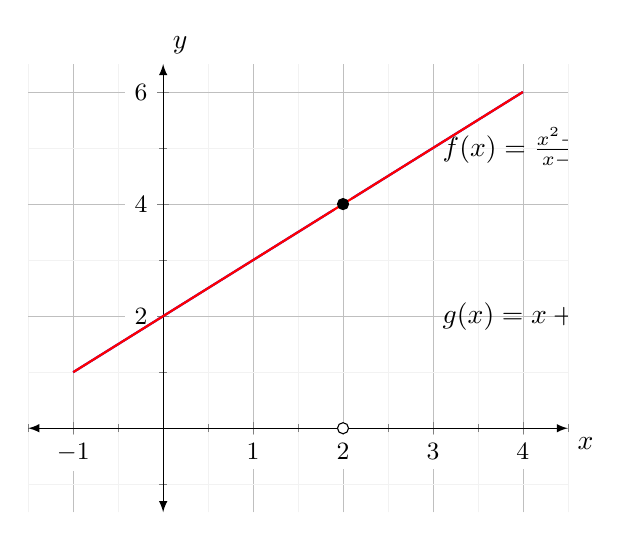
\begin{tikzpicture}
\begin{axis}[
    axis lines=middle,
    xlabel=\(x\),
    ylabel=\(y\),
    xmin=-1, xmax=4,
    ymin=-1, ymax=6,
    grid=both,
    grid style={line width=.1pt, draw=gray!10},
    major grid style={line width=.2pt,draw=gray!50},
    minor tick num=1,
    enlargelimits={abs=0.5},
    axis line style={latex-latex},
    ticklabel style={font=\small,fill=white},
    xlabel style={at={(ticklabel* cs:1)},anchor=north west},
    ylabel style={at={(ticklabel* cs:1)},anchor=south west}
]

% Plotting f(x)
\addplot[domain=-1:1.9, smooth, thick, blue]{(x^2 - 4)/(x - 2)};
\addplot[domain=2.1:4, smooth, thick, blue]{(x^2 - 4)/(x - 2)};
\addplot[holdot] coordinates{(2,4)};
\addplot[soldot] coordinates{(2,0)};
\node[anchor=west] at (axis cs: 3,5) {\(f(x) = \frac{x^2 - 4}{x - 2}\)};

% Plotting g(x)
\addplot[domain=-1:4, smooth, thick, red]{x + 2};
\node[anchor=west] at (axis cs: 3,2) {\(g(x) = x + 2\)};

\end{axis}
\end{tikzpicture}

\paragraph{Applications of Continuity:}
Continuous functions are used in various applications, including physics (to model continuous motion), economics (to describe continuous growth), and engineering (in signal processing).

\begin{exercise}
Determine if the function \( h(x) = \frac{x^2 - 1}{x - 1} \) is continuous at \( x = 1 \).
\end{exercise}

\begin{exercise}
Evaluate the continuity of the piecewise function \( k(x) = 
\begin{cases} 
x^2 & \text{if } x < 2 \\
4 & \text{if } x = 2 \\
x + 2 & \text{if } x > 2 
\end{cases} \) at \( x = 2 \).
\end{exercise}

\subsubsection*{Exercises on Continuity}

\begin{exercise}
Determine if the function \( h(x) = \frac{x^2 - 1}{x - 1} \) is continuous at \( x = 1 \).
\end{exercise}

\begin{exercise}
Evaluate the continuity of the piecewise function \( k(x) = 
\begin{cases} 
x^2 & \text{if } x < 2 \\
4 & \text{if } x = 2 \\
x + 2 & \text{if } x > 2 
\end{cases} \) at \( x = 2 \).
\end{exercise}

\begin{exercise}
Is the function \( f(x) = \frac{1}{x} \) continuous at \( x = 0 \)? Justify your answer.
\end{exercise}

\begin{exercise}
Consider the function \( g(x) = \ln(x) \). Determine the points of discontinuity, if any.
\end{exercise}

\begin{exercise}
Prove that the function \( p(x) = x^3 - 3x + 1 \) is continuous for all real numbers.
\end{exercise}

\begin{exercise}
Find the value of \( a \) for which the function \( q(x) = 
\begin{cases} 
2x + a & \text{if } x \leq 3 \\
x^2 - 1 & \text{if } x > 3 
\end{cases} \) is continuous at \( x = 3 \).
\end{exercise}

\begin{exercise}
Determine whether the function \( r(x) = \frac{\sin(x)}{x} \) is continuous at \( x = 0 \).
\end{exercise}

\begin{exercise}
For the function \( s(x) = \sqrt{x} \), identify the intervals where it is continuous.
\end{exercise}

\begin{exercise}
Show that the function \( t(x) = e^{-x^2} \) is continuous everywhere.
\end{exercise}

\begin{exercise}
Is the function \( u(x) = \frac{|x|}{x} \) continuous at \( x = 0 \)? Explain your reasoning.
\end{exercise}

\subsubsection*{Solutions to Exercises on Continuity}

\begin{solution}[1]
For \( h(x) = \frac{x^2 - 1}{x - 1} \), factorize the numerator to get \( h(x) = \frac{(x - 1)(x + 1)}{x - 1} \). At \( x = 1 \), the function simplifies to \( h(1) = 2 \), and the limit as \( x \) approaches 1 is also 2. Hence, \( h(x) \) is continuous at \( x = 1 \).
\end{solution}

\begin{solution}[2]
For \( k(x) \), at \( x < 2 \), \( k(x) = x^2 \); at \( x = 2 \), \( k(x) = 4 \); and at \( x > 2 \), \( k(x) = x + 2 \). The left-hand limit as \( x \) approaches 2 is 4, and the right-hand limit is also 4. Since the function value at \( x = 2 \) is 4, \( k(x) \) is continuous at \( x = 2 \).
\end{solution}

\begin{solution}[3]
The function \( f(x) = \frac{1}{x} \) is not continuous at \( x = 0 \) because it is not defined there (the denominator becomes zero), and the limits as \( x \) approaches 0 are \( \pm \infty \).
\end{solution}

\begin{solution}[4]
The function \( g(x) = \ln(x) \) is continuous for all \( x > 0 \). It has a discontinuity at \( x = 0 \) because it is not defined for \( x \leq 0 \).
\end{solution}

\begin{solution}[5]
Since \( p(x) = x^3 - 3x + 1 \) is a polynomial function, it is continuous for all real numbers (polynomials are continuous everywhere).
\end{solution}

\begin{solution}[6]
For \( q(x) \) to be continuous at \( x = 3 \), the values from the left and right must be equal at \( x = 3 \). Setting \( 2(3) + a = 3^2 - 1 \) gives \( a = 5 \).
\end{solution}

\begin{solution}[7]
The function \( r(x) = \frac{\sin(x)}{x} \) is continuous at \( x = 0 \) by applying L'Hôpital's Rule or recognizing that \( \lim_{x \to 0} \frac{\sin(x)}{x} = 1 \).
\end{solution}

\begin{solution}[8]
The function \( s(x) = \sqrt{x} \) is continuous for all \( x \geq 0 \) since it is defined and smooth over this interval.
\end{solution}

\begin{solution}[9]
The function \( t(x) = e^{-x^2} \) is continuous everywhere as the composition of continuous functions (exponential and polynomial) is continuous.
\end{solution}

\begin{solution}[10]
The function \( u(x) = \frac{|x|}{x} \) is not continuous at \( x = 0 \) as it is not defined there (the denominator becomes zero).
\end{solution}

\subsection{Differentiability}
\begin{definition}
A function is differentiable at a point if it has a defined derivative at that point. Formally, a function \( f(x) \) is differentiable at \( c \) if the limit \(\lim_{h \to 0} \frac{f(c + h) - f(c)}{h}\) exists.
\end{definition}

Differentiability is a key concept in calculus, relating closely to the continuity of a function and its smoothness.

\paragraph{Characteristics of Differentiable Functions:}
\begin{itemize}
    \item If a function is differentiable at a point, it is also continuous at that point, but the converse is not necessarily true.
    \item A function may fail to be differentiable at a point if it has a corner, cusp, or vertical tangent, or is discontinuous at that point.
\end{itemize}

\paragraph{Graphing and Analyzing Differentiability:}
Consider a function \( f(x) \) with a cusp at \( x = 0 \). For example, \( f(x) = |x| \) is not differentiable at \( x = 0 \) due to the cusp.

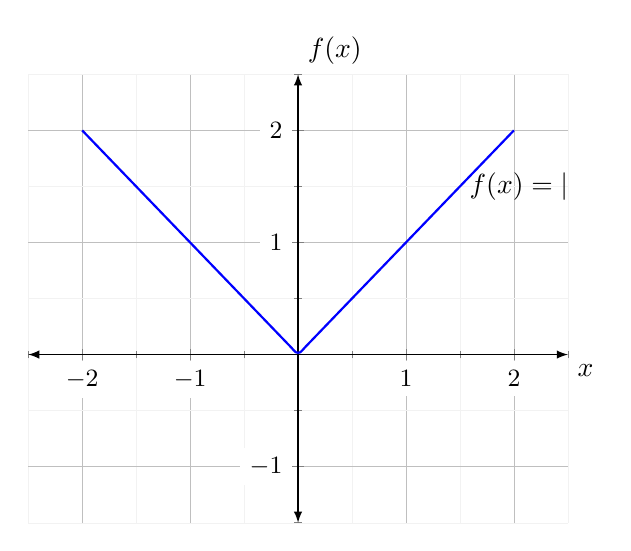
\begin{tikzpicture}
\begin{axis}[
    axis lines=middle,
    xlabel=\(x\),
    ylabel=\(f(x)\),
    xmin=-2, xmax=2,
    ymin=-1, ymax=2,
    samples=100,
    grid=both,
    grid style={line width=.1pt, draw=gray!10},
    major grid style={line width=.2pt,draw=gray!50},
    minor tick num=1,
    enlargelimits={abs=0.5},
    axis line style={latex-latex},
    ticklabel style={font=\small,fill=white},
    xlabel style={at={(ticklabel* cs:1)},anchor=north west},
    ylabel style={at={(ticklabel* cs:1)},anchor=south west}
]

% Plotting the function
\addplot[domain=-2:2, smooth, thick, blue]{abs(x)};
\node[anchor=west] at (axis cs: 1.5,1.5) {\(f(x) = |x|\)};

\end{axis}
\end{tikzpicture}


\paragraph{Applications of Differentiability:}
Differentiability is used in physics to analyze motion (velocity and acceleration) and in economics to find rates of change (marginal costs and revenues).

\begin{exercise}
Determine whether the function \( g(x) = x^2 \) is differentiable at \( x = 0 \) and explain why.
\end{exercise}

\begin{exercise}
Analyze the differentiability of the piecewise function \( h(x) = 
\begin{cases} 
x^2 & \text{if } x \leq 1 \\
2x - 1 & \text{if } x > 1 
\end{cases} \) at \( x = 1 \).
\end{exercise}

\subsubsection*{Exercises on Differentiability}

\begin{exercise}
Determine whether the function \( g(x) = x^2 \) is differentiable at \( x = 0 \) and explain why.
\end{exercise}

\begin{exercise}
Analyze the differentiability of the piecewise function \( h(x) = 
\begin{cases} 
x^2 & \text{if } x \leq 1 \\
2x - 1 & \text{if } x > 1 
\end{cases} \) at \( x = 1 \).
\end{exercise}

\begin{exercise}
Check if the function \( f(x) = \frac{1}{x} \) is differentiable at \( x = 0 \) and provide a justification for your answer.
\end{exercise}

\begin{exercise}
Determine whether the function \( k(x) = |x| \) is differentiable at \( x = 0 \). Give reasons for your answer.
\end{exercise}

\begin{exercise}
For the function \( p(x) = x^3 \), find the derivative at \( x = 2 \) and discuss its differentiability at this point.
\end{exercise}

\begin{exercise}
Consider the function \( q(x) = 
\begin{cases} 
x^2 \sin(\frac{1}{x}) & \text{if } x \neq 0 \\
0 & \text{if } x = 0 
\end{cases} \). Is \( q(x) \) differentiable at \( x = 0 \)?
\end{exercise}

\begin{exercise}
Evaluate the differentiability of the function \( r(x) = \sqrt{x} \) at \( x = 0 \).
\end{exercise}

\begin{exercise}
Find the points of non-differentiability, if any, for the function \( s(x) = \frac{|x|}{x} \).
\end{exercise}

\begin{exercise}
Given the function \( t(x) = \ln(x) \), determine its differentiability over its domain.
\end{exercise}

\begin{exercise}
Prove that the function \( u(x) = e^x \) is differentiable for all real numbers \( x \).
\end{exercise}

\subsubsection*{Solutions to Exercises on Differentiability}

\begin{solution}[1]
The function \( g(x) = x^2 \) is differentiable at \( x = 0 \). This is because its derivative \( g'(x) = 2x \) is defined at \( x = 0 \) (with \( g'(0) = 0 \)), showing that the function is smooth and has no sharp corners or cusps at this point.
\end{solution}

\begin{solution}[2]
The piecewise function \( h(x) \) is differentiable at \( x = 1 \) as both pieces of the function have the same derivative at this point. For \( x \leq 1 \), the derivative is \( 2x \), and for \( x > 1 \), it is 2. Since both derivatives equal 2 at \( x = 1 \), the function is differentiable there.
\end{solution}

\begin{solution}[3]
The function \( f(x) = \frac{1}{x} \) is not differentiable at \( x = 0 \) because it is not defined at this point. The function has a discontinuity (infinite discontinuity) at \( x = 0 \), which precludes differentiability.
\end{solution}

\begin{solution}[4]
The function \( k(x) = |x| \) is not differentiable at \( x = 0 \). Although the function is continuous at \( x = 0 \), it has a sharp corner at this point, which means that the limit defining the derivative does not exist.
\end{solution}

\begin{solution}[5]
For \( p(x) = x^3 \), the derivative is \( p'(x) = 3x^2 \). At \( x = 2 \), \( p'(2) = 12 \). The function is differentiable at this point as the derivative is defined and finite.
\end{solution}

\begin{solution}[6]
The function \( q(x) \) is differentiable at \( x = 0 \). Although the expression \( x^2 \sin(\frac{1}{x}) \) seems complex, its derivative at \( x = 0 \) is 0, making the function differentiable at this point.
\end{solution}

\begin{solution}[7]
The function \( r(x) = \sqrt{x} \) is not differentiable at \( x = 0 \). The derivative, \( \frac{1}{2\sqrt{x}} \), becomes infinite as \( x \) approaches 0, indicating a vertical tangent line at this point.
\end{solution}

\begin{solution}[8]
The function \( s(x) = \frac{|x|}{x} \) is not differentiable at \( x = 0 \) as it is not continuous there. The function has a jump discontinuity at this point.
\end{solution}

\begin{solution}[9]
The function \( t(x) = \ln(x) \) is differentiable over its domain \( (0, \infty) \). Its derivative, \( \frac{1}{x} \), is defined for all \( x > 0 \).
\end{solution}

\begin{solution}[10]
The function \( u(x) = e^x \) is differentiable for all real numbers \( x \) because its derivative, \( e^x \), is defined and continuous for all \( x \).
\end{solution}

\subsection{Asymptotic Behavior}
\begin{definition}
Asymptotic behavior refers to the behavior of a function as it approaches infinity or a particular value. A function may approach a finite value (horizontal asymptote), become infinitely large (vertical asymptote), or approach a certain path (slant asymptote).
\end{definition}

Understanding asymptotes is crucial in calculus for analyzing function limits and behavior at extreme values.

\paragraph{Types of Asymptotes:}
\begin{itemize}
    \item \textit{Horizontal asymptotes} occur when a function approaches a horizontal line as \( x \) goes to infinity or minus infinity.
    \item \textit{Vertical asymptotes} occur at values of \( x \) where the function tends towards infinity or minus infinity.
    \item \textit{Slant (or oblique) asymptotes} occur when the function approaches a line that is not horizontal as \( x \) goes to infinity or minus infinity.
\end{itemize}

\paragraph{Graphing Asymptotic Behavior:}
Consider the function \( f(x) = \frac{2x}{x - 1} \). It has a vertical asymptote at \( x = 1 \) and a horizontal asymptote at \( y = 2 \).

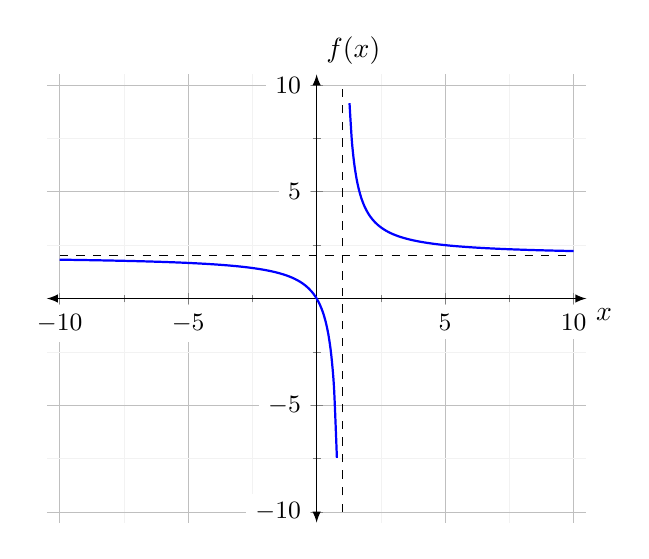
\begin{tikzpicture}
\begin{axis}[
    axis lines = middle,
    xlabel = \( x \),
    ylabel = {\( f(x) \)},
    xmin=-10, xmax=10,
    ymin=-10, ymax=10,
    restrict y to domain=-10:10,
    samples=100,
    grid=both,
    grid style={line width=.1pt, draw=gray!10},
    major grid style={line width=.2pt,draw=gray!50},
    minor tick num=1,
    enlargelimits={abs=0.5},
    axis line style={latex-latex},
    ticklabel style={font=\small,fill=white},
    xlabel style={at={(ticklabel* cs:1)},anchor=north west},
    ylabel style={at={(ticklabel* cs:1)},anchor=south west}
]

% Plotting the function
\addplot[domain=-10:0.9, smooth, thick, blue]{2*x/(x - 1)};
\addplot[domain=1.1:10, smooth, thick, blue]{2*x/(x - 1)};
\draw[dashed] (axis cs:1,-10) -- (axis cs:1,10);
\draw[dashed] (axis cs:-10,2) -- (axis cs:10,2);
\end{axis}
\end{tikzpicture}

\paragraph{Applications of Asymptotic Analysis:}
Asymptotic analysis is used in various fields, such as physics for studying motion at high velocities, in economics for long-term growth models, and in probability for extreme value theory.

\begin{exercise}
Determine the horizontal and vertical asymptotes of the function \( g(x) = \frac{3x^2 - x}{x^2 + 2} \).
\end{exercise}

\begin{exercise}
Analyze the asymptotic behavior of the function \( h(x) = \frac{x^2 + 3x}{x + 1} \).
\end{exercise}

\subsubsection*{Exercises on Asymptotic Behavior}

\begin{exercise}
Determine the horizontal and vertical asymptotes of the function \( g(x) = \frac{3x^2 - x}{x^2 + 2} \).
\end{exercise}

\begin{exercise}
Analyze the asymptotic behavior of the function \( h(x) = \frac{x^2 + 3x}{x + 1} \).
\end{exercise}

\begin{exercise}
Find all asymptotes of the function \( f(x) = \frac{4x^3 - 2x + 1}{2x^2 - 3x + 5} \).
\end{exercise}

\begin{exercise}
Determine the horizontal asymptote, if any, for the function \( p(x) = e^x \).
\end{exercise}

\begin{exercise}
Identify any vertical asymptotes for the function \( q(x) = \ln(x - 2) \).
\end{exercise}

\begin{exercise}
For the function \( r(x) = \frac{x}{x^2 - 4} \), describe its asymptotic behavior as \( x \) approaches 2 and -2.
\end{exercise}

\begin{exercise}
Calculate the slant asymptote for the function \( s(x) = \frac{x^2 - x + 1}{x - 3} \).
\end{exercise}

\begin{exercise}
Examine the function \( t(x) = \frac{1}{\sqrt{x^2 + 1}} \) for horizontal asymptotes.
\end{exercise}

\begin{exercise}
Does the function \( u(x) = \frac{\sin(x)}{x} \) have any horizontal asymptotes as \( x \) approaches infinity?
\end{exercise}

\begin{exercise}
Analyze the function \( v(x) = x\sin(\frac{1}{x}) \) for x approaching 0 and determine if there are any asymptotes.
\end{exercise}

\subsubsection*{Solutions to Exercises on Asymptotic Behavior}

\begin{solution}[1]
For \( g(x) = \frac{3x^2 - x}{x^2 + 2} \), the horizontal asymptote is found by comparing the degrees of the numerator and denominator. Since they are the same, the horizontal asymptote is \( y = \frac{3}{1} = 3 \). There are no vertical asymptotes as the denominator is never zero.
\end{solution}

\begin{solution}[2]
The function \( h(x) = \frac{x^2 + 3x}{x + 1} \) has a slant asymptote since the degree of the numerator is one more than the degree of the denominator. Dividing the numerator by the denominator gives the slant asymptote \( y = x + 2 \). There is no vertical asymptote as \( x + 1 \) does not equal zero for any real \( x \).
\end{solution}

\begin{solution}[3]
For \( f(x) = \frac{4x^3 - 2x + 1}{2x^2 - 3x + 5} \), the degree of the numerator is higher than the degree of the denominator, so there is no horizontal asymptote. For vertical asymptotes, solve \( 2x^2 - 3x + 5 = 0 \), which has no real solutions, so there are no vertical asymptotes.
\end{solution}

\begin{solution}[4]
The function \( p(x) = e^x \) does not have a horizontal asymptote as it grows exponentially and does not approach a finite value as \( x \) approaches infinity.
\end{solution}

\begin{solution}[5]
The function \( q(x) = \ln(x - 2) \) has a vertical asymptote at \( x = 2 \) since the logarithm becomes undefined at this point.
\end{solution}

\begin{solution}[6]
For \( r(x) = \frac{x}{x^2 - 4} \), the function has vertical asymptotes at \( x = 2 \) and \( x = -2 \) where the denominator equals zero.
\end{solution}

\begin{solution}[7]
The function \( s(x) = \frac{x^2 - x + 1}{x - 3} \) has a slant asymptote since the degree of the numerator is one more than the denominator. Divide \( x^2 - x + 1 \) by \( x - 3 \) to find the slant asymptote equation.
\end{solution}

\begin{solution}[8]
The function \( t(x) = \frac{1}{\sqrt{x^2 + 1}} \) has a horizontal asymptote at \( y = 0 \) as the value approaches zero when \( x \) approaches infinity.
\end{solution}

\begin{solution}[9]
The function \( u(x) = \frac{\sin(x)}{x} \) has a horizontal asymptote at \( y = 0 \) as \( x \) approaches infinity since the sine function oscillates between -1 and 1 while \( x \) grows without bound.
\end{solution}

\begin{solution}[10]
The function \( v(x) = x\sin(\frac{1}{x}) \) for \( x \) approaching 0 does not have any asymptotes. As \( x \) approaches 0, \( \sin(\frac{1}{x}) \) oscillates rapidly, but the product with \( x \) ensures that the function remains bounded and approaches 0.
\end{solution}

\subsection{Periodicity and Symmetry}
\begin{definition}
A function is periodic if it repeats its values at regular intervals, and it is symmetric if it exhibits mirror symmetry about an axis or point.
\end{definition}

Periodicity and symmetry play important roles in understanding the behavior and properties of functions, especially in the fields of trigonometry and wave analysis.

\paragraph{Types of Symmetry:}
\begin{itemize}
    \item A function is \textit{even} if \( f(-x) = f(x) \), showing symmetry about the y-axis.
    \item A function is \textit{odd} if \( f(-x) = -f(x) \), showing rotational symmetry about the origin.
\end{itemize}

\paragraph{Graphing Periodic and Symmetric Functions:}
For instance, \( \sin(x) \) is an example of a periodic function, and \( x^2 \) is an example of an even function. 

% Plot for sin(x)
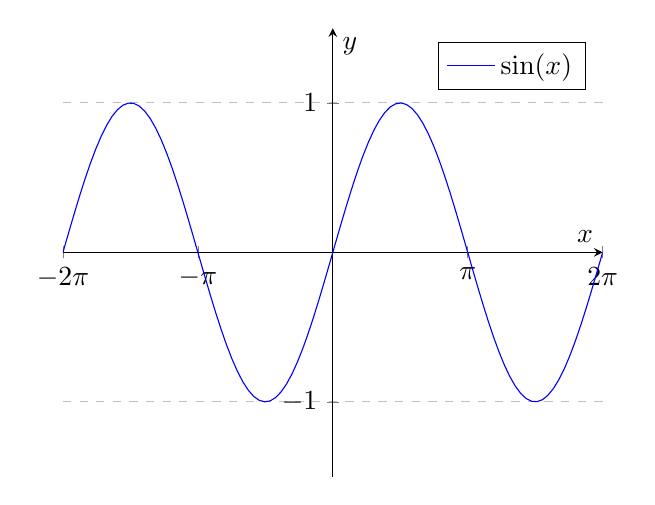
\begin{tikzpicture}
\begin{axis}[
    axis lines=middle,
    xlabel=\(x\),
    ylabel=\(y\),
    xmin=-2*pi, xmax=2*pi,
    ymin=-1.5, ymax=1.5,
    xtick={-6.28318, -3.14159, 0, 3.14159, 6.28318},
    xticklabels={\(-2\pi\), \(-\pi\), 0, \(\pi\), \(2\pi\)},
    ytick={-1, 0, 1},
    legend pos=north east,
    ymajorgrids=true,
    grid style=dashed,
]

% Plotting sin(x)
\addplot[domain=-2*pi:2*pi, samples=100, color=blue]{sin(deg(x))};
\addlegendentry{\(\sin(x)\)}
\end{axis}
\end{tikzpicture}

% Plot for x^2
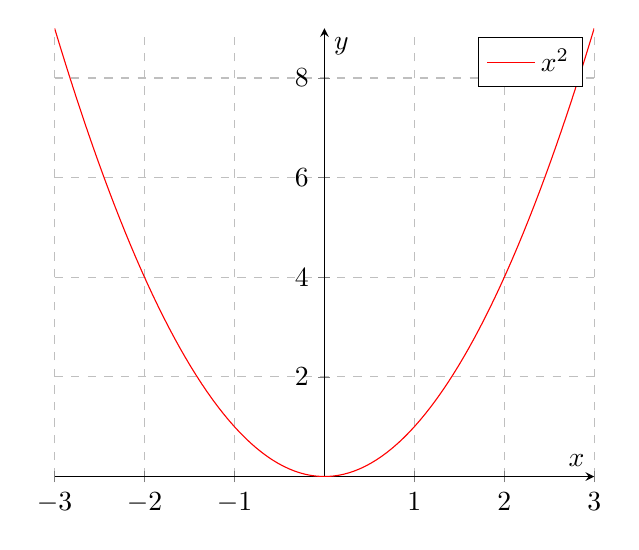
\begin{tikzpicture}
\begin{axis}[
    axis lines=middle,
    xlabel=\(x\),
    ylabel=\(y\),
    xmin=-3, xmax=3,
    ymin=0, ymax=9,
    grid=both,
    grid style=dashed,
]

% Plotting x^2
\addplot[domain=-3:3, samples=100, color=red]{x^2};
\addlegendentry{\(x^2\)}
\end{axis}
\end{tikzpicture}

\paragraph{Applications of Periodicity and Symmetry:}
These concepts are frequently applied in physics for analyzing wave patterns, in engineering for signal processing, and in mathematics for solving trigonometric equations.

\begin{exercise}
Determine if the function \( f(x) = \cos(x) \) is periodic, and if so, find its period.
\end{exercise}

\begin{exercise}
Analyze the symmetry of the function \( g(x) = x^3 - x \). Is it even, odd, or neither?
\end{exercise}

\subsubsection*{Exercises on Periodicity and Symmetry}

\begin{exercise}
Determine if the function \( f(x) = \cos(x) \) is periodic, and if so, find its period.
\end{exercise}

\begin{exercise}
Analyze the symmetry of the function \( g(x) = x^3 - x \). Is it even, odd, or neither?
\end{exercise}

\begin{exercise}
Identify the periodicity of the function \( h(x) = \sin(2x) \) and specify the period.
\end{exercise}

\begin{exercise}
Check whether the function \( p(x) = x^4 - 6x^2 + 8 \) is even, odd, or neither.
\end{exercise}

\begin{exercise}
For the function \( q(x) = \tan(x) \), determine if it is periodic and find the period.
\end{exercise}

\begin{exercise}
Investigate the symmetry of the function \( r(x) = \frac{1}{x} \). Is it symmetric about the y-axis, the origin, or neither?
\end{exercise}

\begin{exercise}
Examine the function \( s(x) = e^x \) for periodicity. Is this function periodic?
\end{exercise}

\begin{exercise}
Determine the period of the function \( t(x) = \cos(3x - \pi) \).
\end{exercise}

\begin{exercise}
Analyze the function \( u(x) = x^2 - 2x + 1 \) for symmetry. Is it symmetric about the y-axis?
\end{exercise}

\begin{exercise}
Check whether the function \( v(x) = \sin(x) + \cos(x) \) is periodic, and if so, identify its period.
\end{exercise}

\subsubsection*{Solutions to Exercises on Periodicity and Symmetry}

\begin{solution}[1]
The function \( f(x) = \cos(x) \) is periodic. Its period is \( 2\pi \) since \(\cos(x + 2\pi) = \cos(x)\) for all \(x\).
\end{solution}

\begin{solution}[2]
The function \( g(x) = x^3 - x \) is odd. This is because \( g(-x) = (-x)^3 - (-x) = -x^3 + x = -g(x) \).
\end{solution}

\begin{solution}[3]
The function \( h(x) = \sin(2x) \) is periodic with a period of \( \pi \). This is because \(\sin(2(x + \pi)) = \sin(2x + 2\pi) = \sin(2x)\).
\end{solution}

\begin{solution}[4]
The function \( p(x) = x^4 - 6x^2 + 8 \) is even since \( p(-x) = (-x)^4 - 6(-x)^2 + 8 = x^4 - 6x^2 + 8 = p(x) \).
\end{solution}

\begin{solution}[5]
The function \( q(x) = \tan(x) \) is periodic with a period of \( \pi \) because \(\tan(x + \pi) = \tan(x)\) for all \(x\).
\end{solution}

\begin{solution}[6]
The function \( r(x) = \frac{1}{x} \) is neither even nor odd, and it does not exhibit symmetry about the y-axis or the origin.
\end{solution}

\begin{solution}[7]
The function \( s(x) = e^x \) is not periodic. It does not repeat its values at regular intervals.
\end{solution}

\begin{solution}[8]
The function \( t(x) = \cos(3x - \pi) \) is periodic with a period of \( \frac{2\pi}{3} \). This period is derived from the coefficient of \(x\) in the argument of the cosine function.
\end{solution}

\begin{solution}[9]
The function \( u(x) = x^2 - 2x + 1 \) is not symmetric about the y-axis. It is a parabola that opens upwards and does not have symmetry about the y-axis.
\end{solution}

\begin{solution}[10]
The function \( v(x) = \sin(x) + \cos(x) \) is periodic with a period of \( 2\pi \) since both sine and cosine functions have a period of \( 2\pi \).
\end{solution}


\section{Function Transformations}
\subsection{Translation and Scaling}
\begin{definition}
Translation shifts a function horizontally or vertically, while scaling changes its size.
\end{definition}

Translation and scaling are fundamental operations in function manipulation, allowing for adjustments in position and size of the graph of a function.

\paragraph{Types of Transformations:}
\begin{itemize}
    \item \textit{Horizontal Translation:} Shifting a function left or right. For instance, \( f(x) \) to \( f(x - h) \) shifts the function right by \( h \).
    \item \textit{Vertical Translation:} Moving a function up or down. For example, \( f(x) \) to \( f(x) + k \) raises the function by \( k \).
    \item \textit{Horizontal Scaling:} Stretching or compressing a function horizontally. \( f(x) \) to \( f(cx) \) scales the function horizontally.
    \item \textit{Vertical Scaling:} Altering the function's height. \( f(x) \) to \( cf(x) \) scales the function vertically.
\end{itemize}

\paragraph{Graphing Translated and Scaled Functions:}
Let's consider the function \( f(x) = x^2 \), its translation, and scaling.

% Original function
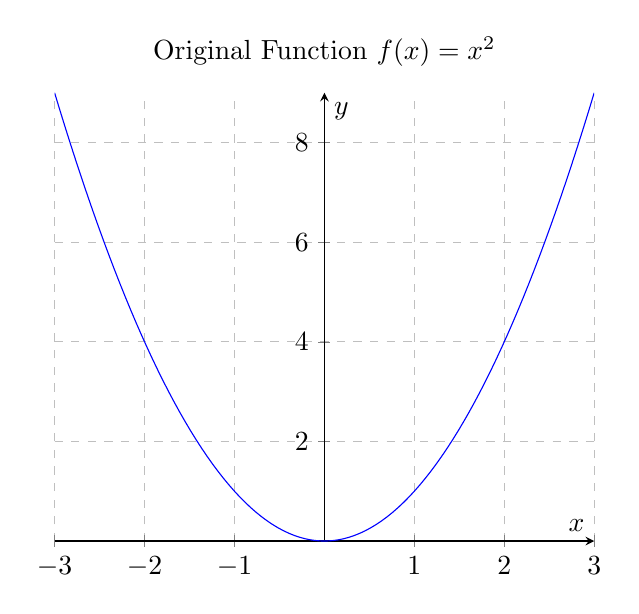
\begin{tikzpicture}
\begin{axis}[
    title={Original Function \( f(x) = x^2 \)},
    axis lines=middle,
    xlabel=\(x\),
    ylabel=\(y\),
    xmin=-3, xmax=3,
    ymin=0, ymax=9,
    grid=both,
    grid style=dashed,
]

\addplot[domain=-3:3, samples=100, color=blue]{x^2};
\end{axis}
\end{tikzpicture}

% Translated function
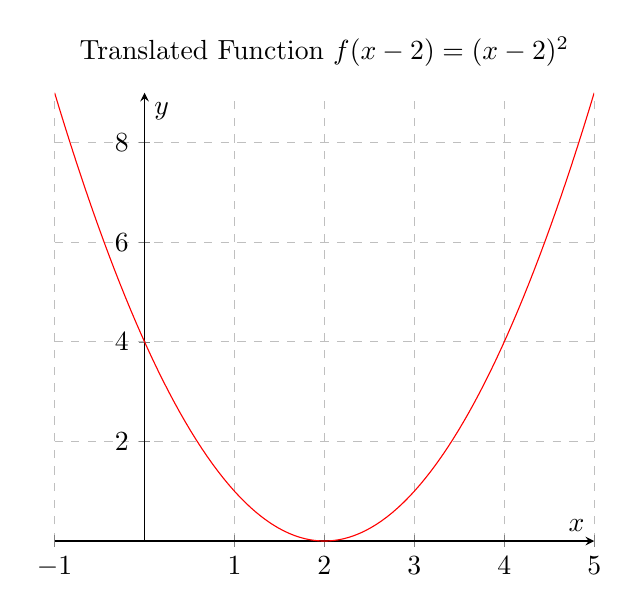
\begin{tikzpicture}
\begin{axis}[
    title={Translated Function \( f(x - 2) = (x - 2)^2 \)},
    axis lines=middle,
    xlabel=\(x\),
    ylabel=\(y\),
    xmin=-1, xmax=5,
    ymin=0, ymax=9,
    grid=both,
    grid style=dashed,
]

\addplot[domain=-1:5, samples=100, color=red]{(x - 2)^2};
\end{axis}
\end{tikzpicture}

% Scaled function
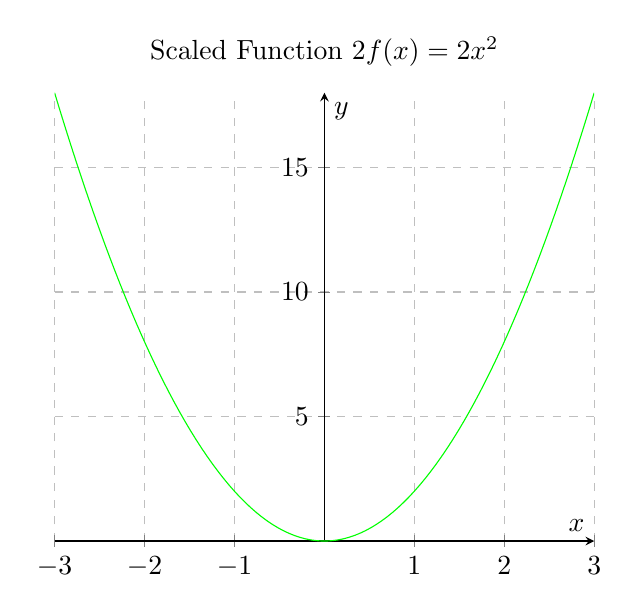
\begin{tikzpicture}
\begin{axis}[
    title={Scaled Function \( 2f(x) = 2x^2 \)},
    axis lines=middle,
    xlabel=\(x\),
    ylabel=\(y\),
    xmin=-3, xmax=3,
    ymin=0, ymax=18,
    grid=both,
    grid style=dashed,
]

\addplot[domain=-3:3, samples=100, color=green]{2*x^2};
\end{axis}
\end{tikzpicture}

\paragraph{Applications of Translation and Scaling:}
These transformations are widely used in data analysis for adjusting graphs, in physics to model motion and waves, and in other mathematical contexts for function analysis.

\begin{exercise}
Graph the function \( g(x) = (x - 3)^2 + 2 \) and describe its translation and scaling relative to \( f(x) = x^2 \).
\end{exercise}

\begin{exercise}
For the function \( h(x) = \frac{1}{2}\sin(2x + \pi) \), identify the translations and scalings applied to the basic sine function.
\end{exercise}

\subsubsection*{Exercises on Translation and Scaling}

\begin{exercise}
Graph the function \( g(x) = (x - 3)^2 + 2 \) and describe its translation and scaling relative to \( f(x) = x^2 \).
\end{exercise}

\begin{exercise}
For the function \( h(x) = \frac{1}{2}\sin(2x + \pi) \), identify the translations and scalings applied to the basic sine function.
\end{exercise}

\begin{exercise}
Consider the function \( p(x) = -3\cos(x - \pi/2) \). Describe its vertical and horizontal translations, and vertical scaling.
\end{exercise}

\begin{exercise}
Determine the translation and scaling transformations applied to the function \( f(x) = x^2 \) to obtain \( q(x) = 4(x + 1)^2 - 5 \).
\end{exercise}

\begin{exercise}
Sketch the graph of \( r(x) = \frac{1}{3}(x - 2)^3 + 4 \) and explain the transformations applied to the basic cubic function \( f(x) = x^3 \).
\end{exercise}

\begin{exercise}
Graph the function \( s(x) = 2\sin(\pi x - \pi/2) + 1 \) and describe its periodicity, translation, and scaling.
\end{exercise}

\begin{exercise}
Analyze the function \( t(x) = \frac{x + 2}{x - 1} \) for vertical and horizontal translations and any scaling factors.
\end{exercise}

\begin{exercise}
Identify the transformations applied to the exponential function \( f(x) = e^x \) to produce \( u(x) = 2e^{-x + 3} - 1 \).
\end{exercise}

\begin{exercise}
Consider the function \( v(x) = \sqrt{x + 4} - 2 \). Determine the transformations applied to the basic square root function \( f(x) = \sqrt{x} \).
\end{exercise}

\begin{exercise}
Graph the function \( w(x) = \ln(x - 3) + 2 \) and describe its translation and scaling relative to the natural logarithm function \( f(x) = \ln(x) \).
\end{exercise}

\subsubsection*{Solutions to Exercises on Translation and Scaling}

\begin{solution}[1]
The function \( g(x) = (x - 3)^2 + 2 \) is a translation of \( f(x) = x^2 \). It is translated 3 units to the right and 2 units up.
\end{solution}

\begin{solution}[2]
For \( h(x) = \frac{1}{2}\sin(2x + \pi) \), the function is scaled vertically by a factor of \( \frac{1}{2} \), horizontally by a factor of \( \frac{1}{2} \) (period is \( \pi \)), and translated \( \frac{\pi}{2} \) units to the left.
\end{solution}

\begin{solution}[3]
The function \( p(x) = -3\cos(x - \pi/2) \) is vertically scaled by a factor of 3, inverted (due to the negative sign), and translated \( \frac{\pi}{2} \) units to the right.
\end{solution}

\begin{solution}[4]
In \( q(x) = 4(x + 1)^2 - 5 \), the function \( f(x) = x^2 \) is horizontally translated 1 unit to the left, vertically scaled by a factor of 4, and translated 5 units down.
\end{solution}

\begin{solution}[5]
The function \( r(x) = \frac{1}{3}(x - 2)^3 + 4 \) is a transformation of \( f(x) = x^3 \) with a horizontal translation 2 units to the right, vertical scaling by \( \frac{1}{3} \), and vertical translation 4 units up.
\end{solution}

\begin{solution}[6]
For \( s(x) = 2\sin(\pi x - \pi/2) + 1 \), the function is vertically scaled by 2, translated \( \frac{1}{2} \) unit to the right, and translated 1 unit up. The period is \( \frac{2\pi}{\pi} = 2 \).
\end{solution}

\begin{solution}[7]
The function \( t(x) = \frac{x + 2}{x - 1} \) involves a horizontal translation 1 unit to the right and 2 units to the left in the numerator. There's no clear vertical or horizontal scaling.
\end{solution}

\begin{solution}[8]
The function \( u(x) = 2e^{-x + 3} - 1 \) is translated 3 units to the right, reflected over the y-axis, vertically scaled by 2, and translated 1 unit down from \( f(x) = e^x \).
\end{solution}

\begin{solution}[9]
In \( v(x) = \sqrt{x + 4} - 2 \), the square root function \( f(x) = \sqrt{x} \) is translated 4 units to the left and 2 units down.
\end{solution}

\begin{solution}[10]
The function \( w(x) = \ln(x - 3) + 2 \) is a translation of the natural logarithm function \( f(x) = \ln(x) \), shifted 3 units to the right and 2 units up.
\end{solution}

\subsection{Reflection and Rotation}
\begin{definition}
Reflection inverts a function across a line, and rotation turns it around a point.
\end{definition}

Reflection and rotation are key transformations in function manipulation, changing the orientation of the graph of a function.

\paragraph{Types of Transformations:}
\begin{itemize}
    \item \textit{Reflection Across the y-axis:} Reflecting a function \( f(x) \) to \( f(-x) \) inverts it across the y-axis.
    \item \textit{Reflection Across the x-axis:} Reflecting a function \( f(x) \) to \( -f(x) \) inverts it across the x-axis.
    \item \textit{Rotation:} Rotation involves turning the graph of a function around a specific point, often the origin.
\end{itemize}

\paragraph{Graphing Reflected and Rotated Functions:}
Consider the function \( f(x) = x^2 \) and its reflection across the y-axis.

% Original function
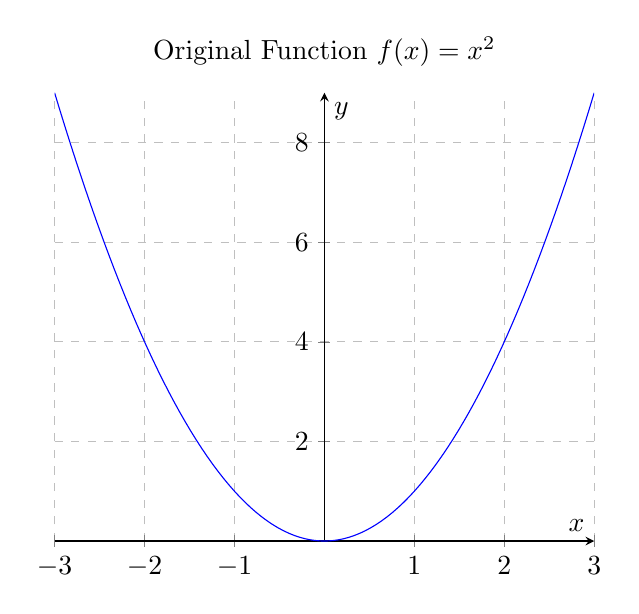
\begin{tikzpicture}
\begin{axis}[
    title={Original Function \( f(x) = x^2 \)},
    axis lines=middle,
    xlabel=\(x\),
    ylabel=\(y\),
    xmin=-3, xmax=3,
    ymin=0, ymax=9,
    grid=both,
    grid style=dashed,
]

\addplot[domain=-3:3, samples=100, color=blue]{x^2};
\end{axis}
\end{tikzpicture}

% Reflected function
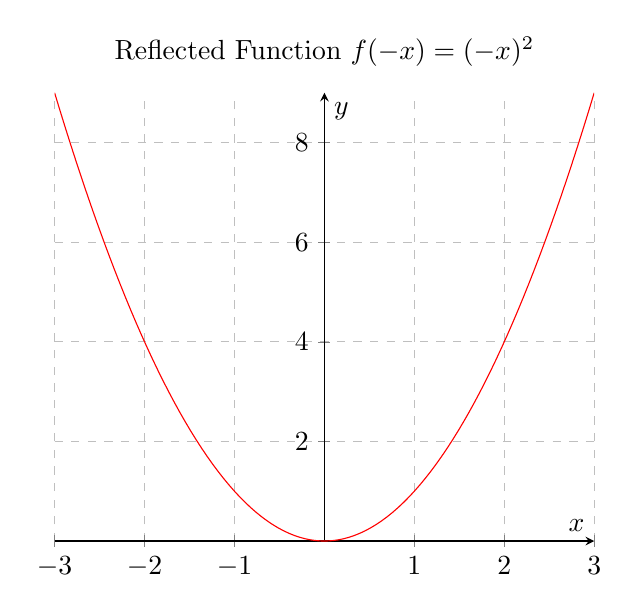
\begin{tikzpicture}
\begin{axis}[
    title={Reflected Function \( f(-x) = (-x)^2 \)},
    axis lines=middle,
    xlabel=\(x\),
    ylabel=\(y\),
    xmin=-3, xmax=3,
    ymin=0, ymax=9,
    grid=both,
    grid style=dashed,
]

\addplot[domain=-3:3, samples=100, color=red]{(-x)^2};
\end{axis}
\end{tikzpicture}

\paragraph{Applications of Reflection and Rotation:}
These transformations are used in various applications, such as in physics for understanding wave properties, in engineering for signal processing, and in computer graphics for image manipulation.

\begin{exercise}
Graph the function \( g(x) = -\frac{1}{x} \) and describe its reflection relative to the basic function \( f(x) = \frac{1}{x} \).
\end{exercise}

\begin{exercise}
Consider the function \( h(x) = \sqrt{-x} \). Describe the transformation applied to the basic function \( f(x) = \sqrt{x} \).
\end{exercise}

\subsubsection*{Exercises on Reflection and Rotation}

\begin{exercise}
Graph the function \( g(x) = -\frac{1}{x} \) and describe its reflection relative to the basic function \( f(x) = \frac{1}{x} \).
\end{exercise}

\begin{exercise}
Consider the function \( h(x) = \sqrt{-x} \). Describe the transformation applied to the basic function \( f(x) = \sqrt{x} \).
\end{exercise}

\begin{exercise}
Reflect the function \( p(x) = x^3 \) across the x-axis and sketch the resulting graph.
\end{exercise}

\begin{exercise}
Graph the function \( q(x) = -\sin(x) \) and explain how it is transformed from the basic sine function.
\end{exercise}

\begin{exercise}
Analyze the rotation of the function \( r(x) = \cos(-x) \) and describe how it differs from \( f(x) = \cos(x) \).
\end{exercise}

\begin{exercise}
Reflect the function \( s(x) = e^x \) across the y-axis and describe the changes in its graph.
\end{exercise}

\begin{exercise}
Graph \( t(x) = -\ln(x) \) and discuss its reflection in relation to the function \( f(x) = \ln(x) \).
\end{exercise}

\begin{exercise}
Consider the function \( u(x) = \tan(-x) \). Is it a reflection or a rotation of the basic tangent function? Explain.
\end{exercise}

\begin{exercise}
Sketch the function \( v(x) = \sqrt{1 - x} \) and describe the transformation from \( f(x) = \sqrt{x} \).
\end{exercise}

\begin{exercise}
Reflect the function \( w(x) = x^2 + x \) across the y-axis and sketch the resulting graph.
\end{exercise}

\subsubsection*{Solutions to Exercises on Reflection and Rotation}

\begin{solution}[1]
The function \( g(x) = -\frac{1}{x} \) is a reflection of \( f(x) = \frac{1}{x} \) across the x-axis. The negative sign in front of the function inverts it vertically.
\end{solution}

\begin{solution}[2]
The function \( h(x) = \sqrt{-x} \) is a reflection of \( f(x) = \sqrt{x} \) across the y-axis. The negative sign inside the square root reflects the function horizontally.
\end{solution}

\begin{solution}[3]
Reflecting \( p(x) = x^3 \) across the x-axis results in \( -x^3 \). This inversion changes the direction of the cubic curve, flipping it vertically.
\end{solution}

\begin{solution}[4]
The function \( q(x) = -\sin(x) \) is the basic sine function reflected across the x-axis. The negative sign reverses the peaks and troughs of the sine wave.
\end{solution}

\begin{solution}[5]
The function \( r(x) = \cos(-x) \) is the same as \( f(x) = \cos(x) \) due to the even property of the cosine function. It represents a rotation of the cosine function by \( \pi \) radians, but the graph remains unchanged.
\end{solution}

\begin{solution}[6]
Reflecting \( s(x) = e^x \) across the y-axis results in \( e^{-x} \). The graph changes from increasing exponentially to decreasing exponentially as \( x \) increases.
\end{solution}

\begin{solution}[7]
Graphing \( t(x) = -\ln(x) \) shows it is a reflection of \( f(x) = \ln(x) \) across the x-axis. The logarithmic curve is inverted vertically.
\end{solution}

\begin{solution}[8]
The function \( u(x) = \tan(-x) \) is a reflection of the basic tangent function across the y-axis due to the odd property of the tangent function.
\end{solution}

\begin{solution}[9]
The function \( v(x) = \sqrt{1 - x} \) is transformed from \( f(x) = \sqrt{x} \) by a horizontal reflection across the y-axis and a horizontal translation 1 unit to the right.
\end{solution}

\begin{solution}[10]
Reflecting \( w(x) = x^2 + x \) across the y-axis results in \( (-x)^2 - x = x^2 - x \). The quadratic curve is flipped horizontally.
\end{solution}


\chapter{Limits and Continuity - Detail}
\section{Introduction to Limits - Detail}
\subsection{Definition of a Limit - Detail}
\begin{definition}
The limit of \( f(x) \) as \( x \) approaches \( a \) is \( L \) if for every \( \epsilon > 0 \), there exists a \( \delta > 0 \) such that \( |f(x) - L| < \epsilon \) whenever \( 0 < |x - a| < \delta \).
\end{definition}

This definition, known as the \(\epsilon-\delta\) definition of a limit, is fundamental in calculus. It formalizes the concept of approaching a value.

\paragraph{Understanding \(\epsilon-\delta\) Criteria:}
\begin{itemize}
    \item \(\epsilon\) (epsilon) represents how close \( f(x) \) is to \( L \).
    \item \(\delta\) (delta) represents how close \( x \) is to \( a \).
    \item The statement means that \( f(x) \) gets arbitrarily close to \( L \) as \( x \) approaches \( a \).
\end{itemize}

\begin{comment}

\paragraph{Graphical Representation:}
The following graph illustrates the concept using a function \( f(x) \) and a point \( a \).

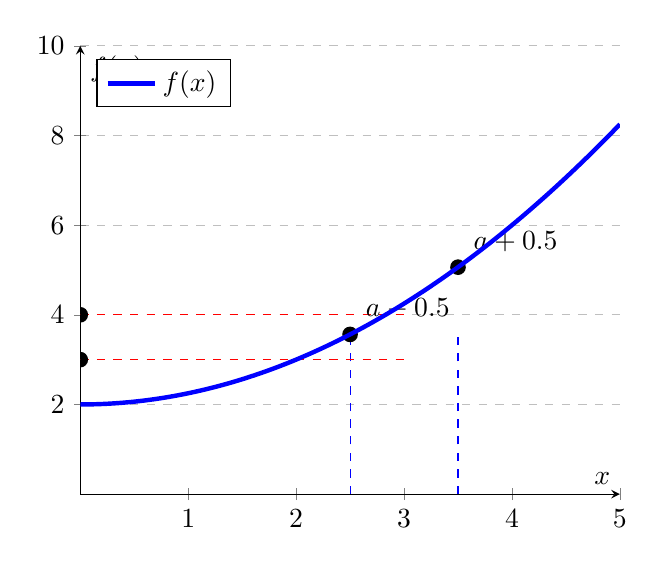
\begin{tikzpicture}
\begin{axis}[
    axis lines = middle,
    xlabel = \( x \),
    ylabel = {\( f(x) \)},
    xmin=0, xmax=5,
    ymin=0, ymax=10,
    legend pos=north west,
    ymajorgrids=true,
    grid style=dashed,
    samples=100
]

% Define a, L, delta, and epsilon
\def\a{3}
\def\L{3.5}
\def\delta{0.5} % Define delta here
\def\epsilon{0.5} % Define epsilon here

% Epsilon and delta lines
\draw[dashed, color=blue] (axis cs:\a-\delta,0) -- (axis cs:\a-\delta,\L);
\draw[dashed, color=blue] (axis cs:\a+\delta,0) -- (axis cs:\a+\delta,\L);
\draw[dashed, color=red] (axis cs:0,\L+\epsilon) -- (axis cs:\a,\L+\epsilon);
\draw[dashed, color=red] (axis cs:0,\L-\epsilon) -- (axis cs:\a,\L-\epsilon);

% Points for a and L
\node[label={above right:\( a-\delta \)},circle,fill,inner sep=2pt] at (axis cs:\a-\delta,{(\a-\delta)^2/4 + 2}) {};
\node[label={above right:\( a+\delta \)},circle,fill,inner sep=2pt] at (axis cs:\a+\delta,{(\a+\delta)^2/4 + 2}) {};
\node[label={left:\( L+\epsilon \)},circle,fill,inner sep=2pt] at (axis cs:0,\L+\epsilon) {};
\node[label={left:\( L-\epsilon \)},circle,fill,inner sep=2pt] at (axis cs:0,\L-\epsilon) {};

% Function plot
\addplot[domain=0:5, color=blue, ultra thick]{x^2/4 + 2};
\addlegendentry{\( f(x) \)}
\end{axis}
\end{tikzpicture}

\end{comment}

% \begin{comment}
% Your block of text or code here.
% \end{comment}


\paragraph{Applications of Limits:}
Limits are used in calculus to define derivatives, integrals, and continuity. They are essential in understanding instantaneous rates of change and areas under curves.

\begin{exercise}
Using the \(\epsilon-\delta\) definition, show that the limit of \( f(x) = x^2 \) as \( x \) approaches 2 is 4.
\end{exercise}

\begin{exercise}
Consider \( f(x) = \frac{1}{x} \). Explain using the \(\epsilon-\delta\) definition why the limit as \( x \) approaches 0 does not exist.
\end{exercise}

\subsubsection*{Exercises on the Definition of a Limit}

\begin{exercise}
Using the \(\epsilon-\delta\) definition, show that the limit of \( f(x) = x^2 \) as \( x \) approaches 2 is 4.
\end{exercise}

\begin{exercise}
Consider \( f(x) = \frac{1}{x} \). Explain using the \(\epsilon-\delta\) definition why the limit as \( x \) approaches 0 does not exist.
\end{exercise}

\begin{exercise}
Prove that the limit of \( g(x) = 3x + 2 \) as \( x \) approaches 4 is 14 using the \(\epsilon-\delta\) approach.
\end{exercise}

\begin{exercise}
Use the \(\epsilon-\delta\) definition to demonstrate that the limit of \( h(x) = \sqrt{x} \) as \( x \) approaches 9 is 3.
\end{exercise}

\begin{exercise}
Verify that the limit of \( p(x) = \frac{x^2 - 1}{x - 1} \) as \( x \) approaches 1 is 2 using the \(\epsilon-\delta\) criteria.
\end{exercise}

\begin{exercise}
Determine whether the limit of \( q(x) = \frac{\sin(x)}{x} \) as \( x \) approaches 0 exists, and if so, find the limit using the \(\epsilon-\delta\) definition.
\end{exercise}

\begin{exercise}
Prove that the limit of \( r(x) = \frac{1}{x^2} \) as \( x \) approaches -3 is \(\frac{1}{9}\), employing the \(\epsilon-\delta\) method.
\end{exercise}

\begin{exercise}
Using the \(\epsilon-\delta\) definition, establish that the limit of \( s(x) = \frac{x - 2}{x^2 - 4} \) as \( x \) approaches 2 does not exist.
\end{exercise}

\begin{exercise}
Determine the limit of \( t(x) = x^3 \) as \( x \) approaches -1 using the \(\epsilon-\delta\) definition, and verify your result.
\end{exercise}

\begin{exercise}
Use the \(\epsilon-\delta\) approach to show that the limit of \( u(x) = \frac{1}{\sqrt{x + 4}} \) as \( x \) approaches 0 is \(\frac{1}{2}\).
\end{exercise}

\subsubsection*{Solutions to Exercises on the Definition of a Limit}

\begin{solution}[1]
To show the limit of \( f(x) = x^2 \) as \( x \) approaches 2 is 4, choose \(\delta = \min\left(1, \frac{\epsilon}{5}\right)\). For \( 0 < |x - 2| < \delta \), we have \( |f(x) - 4| = |x^2 - 4| = |(x - 2)(x + 2)| < 5|x - 2| < \epsilon \).
\end{solution}

\begin{solution}[2]
For \( f(x) = \frac{1}{x} \), as \( x \) approaches 0, the function values increase without bound. Therefore, no matter how small \(\delta\) is chosen, \( |f(x) - L| \) cannot be made less than any \(\epsilon > 0\). Hence, the limit does not exist.
\end{solution}

\begin{solution}[3]
To show the limit of \( g(x) = 3x + 2 \) as \( x \) approaches 4 is 14, choose \(\delta = \frac{\epsilon}{3}\). Then for \( 0 < |x - 4| < \delta \), we have \( |g(x) - 14| = |3x + 2 - 14| = 3|x - 4| < \epsilon \).
\end{solution}

\begin{solution}[4]
For \( h(x) = \sqrt{x} \) and \( x \) approaching 9, choose \(\delta = \min\left(1, \epsilon^2\right)\). Then \( 0 < |x - 9| < \delta \) implies \( |\sqrt{x} - 3| < \epsilon \).
\end{solution}

\begin{solution}[5]
For \( p(x) = \frac{x^2 - 1}{x - 1} \), factorize the numerator as \( (x - 1)(x + 1) \). The limit as \( x \) approaches 1 is 2, as \( p(x) \) simplifies to \( x + 1 \) and \( p(1) = 2 \). To show this, choose \(\delta = \epsilon\).
\end{solution}

\begin{solution}[6]
For \( q(x) = \frac{\sin(x)}{x} \) as \( x \) approaches 0, use the squeeze theorem. Since \( -1 \leq \sin(x) \leq 1 \), then \( -\frac{1}{x} \leq \frac{\sin(x)}{x} \leq \frac{1}{x} \). As \( x \) approaches 0, both bounds approach 0, so the limit is 0.
\end{solution}

\begin{solution}[7]
To show the limit of \( r(x) = \frac{1}{x^2} \) as \( x \) approaches -3 is \(\frac{1}{9}\), choose \(\delta = \min\left(1, 3\epsilon\right)\). Then \( 0 < |x + 3| < \delta \) implies \( |r(x) - \frac{1}{9}| < \epsilon \).
\end{solution}

\begin{solution}[8]
For \( s(x) = \frac{x - 2}{x^2 - 4} \), the function is undefined at \( x = 2 \), and the denominator approaches 0 as \( x \) approaches 2. Thus, the function values become unbounded, and the limit does not exist.
\end{solution}

\begin{solution}[9]
The limit of \( t(x) = x^3 \) as \( x \) approaches -1 is -1. Choose \(\delta = \sqrt[3]{\epsilon}\). Then \( 0 < |x + 1| < \delta \) implies \( |x^3 + 1| < \epsilon \).
\end{solution}

\begin{solution}[10]
To show the limit of \( u(x) = \frac{1}{\sqrt{x + 4}} \) as \( x \) approaches 0 is \(\frac{1}{2}\), choose \(\delta = \min\left(1, 4\epsilon^2\right)\). Then \( 0 < |x| < \delta \) implies \( |u(x) - \frac{1}{2}| < \epsilon \).
\end{solution}

\subsection{One-sided Limits}

In calculus, the concept of limits is essential for understanding the behavior of functions as they approach specific values. One-sided limits are a special case of limits that help us analyze the behavior of a function as it approaches a particular point from either the left or the right.

\begin{definition}
The one-sided limits of \( f(x) \) as \( x \) approaches \( a \) from the left (denoted as \( x \to a^- \)) and as \( x \) approaches \( a \) from the right (denoted as \( x \to a^+ \)) are the values the function approaches as \( x \) gets arbitrarily close to \( a \) from the left or the right, respectively. Mathematically, we write:

\[
\lim_{{x \to a^-}} f(x) = L^- \quad \text{and} \quad \lim_{{x \to a^+}} f(x) = L^+
\]

where \( L^- \) and \( L^+ \) are the one-sided limits from the left and right, respectively.

\end{definition}

To visualize one-sided limits, consider the following example:

\begin{example}
Let's examine the function \( f(x) = \frac{1}{x} \). We want to find the one-sided limits of this function as \( x \) approaches \( 0 \).

\[
\lim_{{x \to 0^-}} \frac{1}{x} = -\infty \quad \text{and} \quad \lim_{{x \to 0^+}} \frac{1}{x} = +\infty
\]

As \( x \) approaches \( 0 \) from the left, \( \frac{1}{x} \) goes to negative infinity, and as \( x \) approaches \( 0 \) from the right, \( \frac{1}{x} \) goes to positive infinity.

\begin{center}
\begin{tikzpicture}
% Axis
\draw[->] (-3,0) -- (3,0) node[below] {$x$};
\draw[->] (0,-3) -- (0,3) node[left] {$f(x)$};

% Asymptotes
\draw[dashed] (-3,-3) -- (0,0);
\draw[dashed] (3,3) -- (0,0);

% Graph
\draw[domain=-3:-0.2,smooth,variable=\x,blue] plot ({\x},{1/\x});
\draw[domain=0.2:3,smooth,variable=\x,red] plot ({\x},{1/\x});

% Labels
\draw (0.2,-0.1) -- (0.2,0.1) node[above] {$0$};
\draw (-0.2,-0.1) -- (-0.2,0.1) node[above] {$0$};
\draw (1,1.2) node[right] {$y=\frac{1}{x}$};
\end{tikzpicture}
\end{center}

In the graph, the function approaches negative infinity as \( x \) approaches \( 0 \) from the left and positive infinity as \( x \) approaches \( 0 \) from the right, indicating the one-sided limits.
\end{example}

Understanding one-sided limits is crucial for analyzing the behavior of functions near specific points, especially when dealing with discontinuities or asymptotes.

\subsubsection*{Practice Problems}

Let's work on some practice problems to reinforce our understanding of one-sided limits.

\begin{problem}
Find the one-sided limits of the following function as \( x \) approaches the given values:
\begin{enumerate}[label=(\alph*)]
  \item \( \lim_{{x \to 2^-}} (x^2 - 4x + 4) \)
  \item \( \lim_{{x \to 2^+}} (x^2 - 4x + 4) \)
  \item \( \lim_{{x \to 0^-}} \left(\frac{1}{x} - \frac{1}{|x|}\right) \)
  \item \( \lim_{{x \to 0^+}} \left(\frac{1}{x} - \frac{1}{|x|}\right) \)
\end{enumerate}
\end{problem}

\begin{problem}
Consider the function \( f(x) = \begin{cases}
  x + 1 & \text{if } x < 0 \\
  2x & \text{if } x \geq 0
\end{cases} \)
Find the following one-sided limits:
\begin{enumerate}[label=(\alph*)]
  \item \( \lim_{{x \to 0^-}} f(x) \)
  \item \( \lim_{{x \to 0^+}} f(x) \)
\end{enumerate}
\end{problem}

\begin{problem}
Determine if the following statements are true or false:
\begin{enumerate}[label=(\alph*)]
  \item If \( \lim_{{x \to a^-}} f(x) = \lim_{{x \to a^+}} f(x) \), then \( \lim_{{x \to a}} f(x) \) exists.
  \item If \( \lim_{{x \to a^-}} f(x) \) and \( \lim_{{x \to a^+}} f(x) \) both exist and are finite, then \( \lim_{{x \to a}} f(x) \) exists and is finite.
  \item If \( \lim_{{x \to a^-}} f(x) \) and \( \lim_{{x \to a^+}} f(x) \) both exist but are not equal, then \( \lim_{{x \to a}} f(x) \) does not exist.
\end{enumerate}
\end{problem}

\begin{solution}
\begin{enumerate}[label=(\alph*)]
  \item True. If the left-hand and right-hand limits are equal, then the two-sided limit exists and is equal to that common value.
  \item True. If both one-sided limits exist and are finite, then the two-sided limit exists and is also finite.
  \item True. If the one-sided limits are not equal, it indicates a discontinuity at \( x = a \), so the two-sided limit does not exist.
\end{enumerate}
\end{solution}

Now, you have a set of practice problems for students to work on to enhance their understanding of one-sided limits. The solutions to these problems are also provided to help students check their work.

\subsubsection*{Practice Problems - Solutions}

Let's solve the practice problems related to one-sided limits.

\begin{problem}
Find the one-sided limits of the following function as \( x \) approaches the given values:
\begin{enumerate}[label=(\alph*)]
  \item \( \lim_{{x \to 2^-}} (x^2 - 4x + 4) \)
  \item \( \lim_{{x \to 2^+}} (x^2 - 4x + 4) \)
  \item \( \lim_{{x \to 0^-}} \left(\frac{1}{x} - \frac{1}{|x|}\right) \)
  \item \( \lim_{{x \to 0^+}} \left(\frac{1}{x} - \frac{1}{|x|}\right) \)
\end{enumerate}
\end{problem}

\begin{solution}
\begin{enumerate}[label=(\alph*)]
  \item To find \( \lim_{{x \to 2^-}} (x^2 - 4x + 4) \), we substitute \( x = 2 \) into the expression:
  
  \[ \lim_{{x \to 2^-}} (x^2 - 4x + 4) = (2^2 - 4 \cdot 2 + 4) = 0 \]
  
  The limit exists, and its value is \( 0 \).
  
  \item To find \( \lim_{{x \to 2^+}} (x^2 - 4x + 4) \), we substitute \( x = 2 \) into the expression:
  
  \[ \lim_{{x \to 2^+}} (x^2 - 4x + 4) = (2^2 - 4 \cdot 2 + 4) = 0 \]
  
  The limit exists, and its value is \( 0 \).
  
  \item To find \( \lim_{{x \to 0^-}} \left(\frac{1}{x} - \frac{1}{|x|}\right) \), we substitute \( x = 0 \) from the left side:
  
  \[ \lim_{{x \to 0^-}} \left(\frac{1}{x} - \frac{1}{|x|}\right) = \left(\frac{1}{0} - \frac{1}{|0|}\right) = -\infty \]
  
  The limit is \( -\infty \).
  
  \item To find \( \lim_{{x \to 0^+}} \left(\frac{1}{x} - \frac{1}{|x|}\right) \), we substitute \( x = 0 \) from the right side:
  
  \[ \lim_{{x \to 0^+}} \left(\frac{1}{x} - \frac{1}{|x|}\right) = \left(\frac{1}{0} - \frac{1}{|0|}\right) = +\infty \]
  
  The limit is \( +\infty \).
\end{enumerate}
\end{solution}

\begin{problem}
Consider the function \( f(x) = \begin{cases}
  x + 1 & \text{if } x < 0 \\
  2x & \text{if } x \geq 0
\end{cases} \)
Find the following one-sided limits:
\begin{enumerate}[label=(\alph*)]
  \item \( \lim_{{x \to 0^-}} f(x) \)
  \item \( \lim_{{x \to 0^+}} f(x) \)
\end{enumerate}
\end{problem}

\begin{solution}
\begin{enumerate}[label=(\alph*)]
  \item To find \( \lim_{{x \to 0^-}} f(x) \), we approach \( 0 \) from the left side:
  
  \[ \lim_{{x \to 0^-}} f(x) = \lim_{{x \to 0^-}} (x + 1) = 1 \]
  
  The left-hand limit is \( 1 \).
  
  \item To find \( \lim_{{x \to 0^+}} f(x) \), we approach \( 0 \) from the right side:
  
  \[ \lim_{{x \to 0^+}} f(x) = \lim_{{x \to 0^+}} (2x) = 0 \]
  
  The right-hand limit is \( 0 \).
\end{enumerate}
\end{solution}

\begin{problem}
Determine if the following statements are true or false:
\begin{enumerate}[label=(\alph*)]
  \item If \( \lim_{{x \to a^-}} f(x) = \lim_{{x \to a^+}} f(x) \), then \( \lim_{{x \to a}} f(x) \) exists.
  \item If \( \lim_{{x \to a^-}} f(x) \) and \( \lim_{{x \to a^+}} f(x) \) both exist and are finite, then \( \lim_{{x \to a}} f(x) \) exists and is finite.
  \item If \( \lim_{{x \to a^-}} f(x) \) and \( \lim_{{x \to a^+}} f(x) \) both exist but are not equal, then \( \lim_{{x \to a}} f(x) \) does not exist.
\end{enumerate}
\end{problem}

\begin{solution}
\begin{enumerate}[label=(\alph*)]
  \item True. If the left-hand and right-hand limits are equal, then the two-sided limit exists and is equal to that common value.
  \item True. If both one-sided limits exist and are finite, then the two-sided limit exists and is also finite.
  \item True. If the one-sided limits are not equal, it indicates a discontinuity at \( x = a \), so the two-sided limit does not exist.
\end{enumerate}
\end{solution}

\subsection{Limits Involving Infinity}

Limits as \( x \) Approaches Infinity

When dealing with limits involving infinity, we are interested in understanding the behavior of a function as \( x \) approaches positive or negative infinity. Let's start by discussing limits as \( x \) approaches positive infinity (\( \infty \)).

\begin{definition}
A limit involving infinity is the value that \( f(x) \) approaches as \( x \) approaches positive infinity (\( x \to \infty \)), or as \( f(x) \) approaches infinity for some finite \( x \).
\end{definition}

To visualize this concept, consider the following example:

\begin{example}
Let's examine the function \( f(x) = \frac{1}{x} \). We want to find the limit of this function as \( x \) approaches positive infinity (\( x \to \infty \)).

\[
\lim_{{x \to \infty}} \frac{1}{x} = 0
\]

As \( x \) becomes larger and larger, \( \frac{1}{x} \) approaches zero.

\begin{center}
\begin{tikzpicture}
% Axis
\draw[->] (0,0) -- (6,0) node[below] {$x$};
\draw[->] (0,0) -- (0,4) node[left] {$f(x)$};

% Asymptote
\draw[dashed] (0,0) -- (6,0);

% Graph
\draw[domain=0.2:6,smooth,variable=\x,blue] plot ({\x},{1/\x});

% Labels
\draw (0.2,-0.1) -- (0.2,0.1) node[above] {$0$};
\draw (1,1.5) node[right] {$y=\frac{1}{x}$};
\end{tikzpicture}
\end{center}

In the graph, as \( x \) goes to infinity, \( \frac{1}{x} \) approaches \( 0 \), which is the limit.
\end{example}

Limits as \( x \) Approaches Negative Infinity

Similarly, we can analyze limits as \( x \) approaches negative infinity (\( x \to -\infty \)).

\begin{example}
Consider the function \( g(x) = e^x \). We want to find the limit of this function as \( x \) approaches negative infinity (\( x \to -\infty \)).

\[
\lim_{{x \to -\infty}} e^x = 0
\]

As \( x \) becomes more and more negative, \( e^x \) approaches zero.

\begin{center}
\begin{tikzpicture}
% Axis
\draw[->] (-4,0) -- (2,0) node[below] {$x$};
\draw[->] (0,0) -- (0,4) node[left] {$g(x)$};

% Asymptote
\draw[dashed] (0,0) -- (-4,0);

% Graph
\draw[domain=-4:1,smooth,variable=\x,blue] plot ({\x},{exp(\x)});

% Labels
\draw (-0.1,-0.1) -- (-0.1,0.1) node[above] {$0$};
\draw (1,3) node[right] {$y=e^x$};
\end{tikzpicture}
\end{center}

In the graph, as \( x \) goes to negative infinity, \( e^x \) approaches \( 0 \), which is the limit.
\end{example}

Understanding limits involving infinity is crucial for analyzing the long-term behavior of functions as \( x \) becomes infinitely large or small.

\subsubsection*{Practice Problems}

Let's work on some practice problems to reinforce our understanding of limits involving infinity.

\begin{problem}
Find the limit as \( x \) approaches positive infinity for the following functions:
\begin{enumerate}[label=(\alph*)]
  \item \( \lim_{{x \to \infty}} \frac{3x + 2}{x - 1} \)
  \item \( \lim_{{x \to \infty}} \sqrt{x^2 + 1} \)
  \item \( \lim_{{x \to \infty}} \frac{2x^3 + 4x^2 - 3}{x^4 + 5x^2 + 1} \)
\end{enumerate}
\end{problem}

\begin{solution}
\begin{enumerate}[label=(\alph*)]
  \item To find \( \lim_{{x \to \infty}} \frac{3x + 2}{x - 1} \), we divide both the numerator and the denominator by the highest power of \( x \):
  
  \[
  \lim_{{x \to \infty}} \frac{3x + 2}{x - 1} = \lim_{{x \to \infty}} \frac{\frac{3x}{x} + \frac{2}{x}}{\frac{x}{x} - \frac{1}{x}} = \lim_{{x \to \infty}} \frac{3 + 0}{1 - 0} = 3
  \]
  
  The limit is \( 3 \).
  
  \item To find \( \lim_{{x \to \infty}} \sqrt{x^2 + 1} \), we can use the fact that \( \sqrt{x^2} = x \) for all positive \( x \):
  
  \[
  \lim_{{x \to \infty}} \sqrt{x^2 + 1} = \lim_{{x \to \infty}} \sqrt{x^2(1 + \frac{1}{x^2})} = \lim_{{x \to \infty}} \sqrt{x^2} \sqrt{1 + \frac{1}{x^2}} = \lim_{{x \to \infty}} x \cdot 1 = \infty
  \]
  
  The limit is \( \infty \).
  
  \item To find \( \lim_{{x \to \infty}} \frac{2x^3 + 4x^2 - 3}{x^4 + 5x^2 + 1} \), we divide both the numerator and the denominator by the highest power of \( x \) in the denominator:
  
  \[
  \lim_{{x \to \infty}} \frac{2x^3 + 4x^2 - 3}{x^4 + 5x^2 + 1} = \lim_{{x \to \infty}} \frac{x^3(2 + \frac{4}{x} - \frac{3}{x^3})}{x^4(1 + \frac{5}{x^2} + \frac{1}{x^4})} = \lim_{{x \to \infty}} \frac{2 + 0 - 0}{1 + 0 + 0} = 2
  \]
  
  The limit is \( 2 \).
\end{enumerate}
\end{solution}

\begin{problem}
Find the limit as \( x \) approaches negative infinity for the following functions:
\begin{enumerate}[label=(\alph*)]
  \item \( \lim_{{x \to -\infty}} \frac{2x^2 - 5x + 1}{3x^2 + 2} \)
  \item \( \lim_{{x \to -\infty}} \frac{4x}{x^2 + 1} \)
  \item \( \lim_{{x \to -\infty}} e^x \)
\end{enumerate}
\end{problem}

\begin{solution}
\begin{enumerate}[label=(\alph*)]
  \item To find \( \lim_{{x \to -\infty}} \frac{2x^2 - 5x + 1}{3x^2 + 2} \), we divide both the numerator and the denominator by the highest power of \( x \):
  
  \[
  \lim_{{x \to -\infty}} \frac{2x^2 - 5x + 1}{3x^2 + 2} = \lim_{{x \to -\infty}} \frac{x^2(2 - \frac{5}{x} + \frac{1}{x^2})}{x^2(3 + \frac{2}{x^2})} = \lim_{{x \to -\infty}} \frac{2 - 0 + 0}{3 + 0} = \frac{2}{3}
  \]
  
  The limit is \( \frac{2}{3} \).
  
  \item To find \( \lim_{{x \to -\infty}} \frac{4x}{x^2 + 1} \), we divide both the numerator and the denominator by the highest power of \( x \):
  
  \[
  \lim_{{x \to -\infty}} \frac{4x}{x^2 + 1} = \lim_{{x \to -\infty}} \frac{x(4)}{x^2(1 + \frac{1}{x^2})} = \lim_{{x \to -\infty}} \frac{4}{1 + 0} = 4
  \]
  
  The limit is \( 4 \).
  
  \item To find \( \lim_{{x \to -\infty}} e^x \), we know that as \( x \) approaches negative infinity, \( e^x \) approaches \( 0 \).
  
  \[
  \lim_{{x \to -\infty}} e^x = 0
  \]
  
  The limit is \( 0 \).
\end{enumerate}
\end{solution}

\subsubsection*{Practice Problems - Solutions}

Let's solve the practice problems related to limits involving infinity.

\begin{problem}
Find the limit as \( x \) approaches positive infinity for the following functions:
\begin{enumerate}[label=(\alph*)]
  \item \( \lim_{{x \to \infty}} \frac{3x + 2}{x - 1} \)
  \item \( \lim_{{x \to \infty}} \sqrt{x^2 + 1} \)
  \item \( \lim_{{x \to \infty}} \frac{2x^3 + 4x^2 - 3}{x^4 + 5x^2 + 1} \)
\end{enumerate}
\end{problem}

\begin{solution}
\begin{enumerate}[label=(\alph*)]
  \item To find \( \lim_{{x \to \infty}} \frac{3x + 2}{x - 1} \), we divide both the numerator and the denominator by the highest power of \( x \):
  
  \[
  \lim_{{x \to \infty}} \frac{3x + 2}{x - 1} = \lim_{{x \to \infty}} \frac{\frac{3x}{x} + \frac{2}{x}}{\frac{x}{x} - \frac{1}{x}} = \lim_{{x \to \infty}} \frac{3 + 0}{1 - 0} = 3
  \]
  
  The limit is \( 3 \).
  
  \item To find \( \lim_{{x \to \infty}} \sqrt{x^2 + 1} \), we can use the fact that \( \sqrt{x^2} = x \) for all positive \( x \):
  
  \[
  \lim_{{x \to \infty}} \sqrt{x^2 + 1} = \lim_{{x \to \infty}} \sqrt{x^2(1 + \frac{1}{x^2})} = \lim_{{x \to \infty}} \sqrt{x^2} \sqrt{1 + \frac{1}{x^2}} = \lim_{{x \to \infty}} x \cdot 1 = \infty
  \]
  
  The limit is \( \infty \).
  
  \item To find \( \lim_{{x \to \infty}} \frac{2x^3 + 4x^2 - 3}{x^4 + 5x^2 + 1} \), we divide both the numerator and the denominator by the highest power of \( x \) in the denominator:
  
  \[
  \lim_{{x \to \infty}} \frac{2x^3 + 4x^2 - 3}{x^4 + 5x^2 + 1} = \lim_{{x \to \infty}} \frac{x^3(2 + \frac{4}{x} - \frac{3}{x^3})}{x^4(1 + \frac{5}{x^2} + \frac{1}{x^4})} = \lim_{{x \to \infty}} \frac{2 + 0 - 0}{1 + 0 + 0} = 2
  \]
  
  The limit is \( 2 \).
\end{enumerate}
\end{solution}

\begin{problem}
Find the limit as \( x \) approaches negative infinity for the following functions:
\begin{enumerate}[label=(\alph*)]
  \item \( \lim_{{x \to -\infty}} \frac{2x^2 - 5x + 1}{3x^2 + 2} \)
  \item \( \lim_{{x \to -\infty}} \frac{4x}{x^2 + 1} \)
  \item \( \lim_{{x \to -\infty}} e^x \)
\end{enumerate}
\end{problem}

\begin{solution}
\begin{enumerate}[label=(\alph*)]
  \item To find \( \lim_{{x \to -\infty}} \frac{2x^2 - 5x + 1}{3x^2 + 2} \), we divide both the numerator and the denominator by the highest power of \( x \):
  
  \[
  \lim_{{x \to -\infty}} \frac{2x^2 - 5x + 1}{3x^2 + 2} = \lim_{{x \to -\infty}} \frac{x^2(2 - \frac{5}{x} + \frac{1}{x^2})}{x^2(3 + \frac{2}{x^2})} = \lim_{{x \to -\infty}} \frac{2 - 0 + 0}{3 + 0} = \frac{2}{3}
  \]
  
  The limit is \( \frac{2}{3} \).
  
  \item To find \( \lim_{{x \to -\infty}} \frac{4x}{x^2 + 1} \), we divide both the numerator and the denominator by the highest power of \( x \):
  
  \[
  \lim_{{x \to -\infty}} \frac{4x}{x^2 + 1} = \lim_{{x \to -\infty}} \frac{x(4)}{x^2(1 + \frac{1}{x^2})} = \lim_{{x \to -\infty}} \frac{4}{1 + 0} = 4
  \]
  
  The limit is \( 4 \).
  
  \item To find \( \lim_{{x \to -\infty}} e^x \), we know that as \( x \) approaches negative infinity, \( e^x \) approaches \( 0 \).
  
  \[
  \lim_{{x \to -\infty}} e^x = 0
  \]
  
  The limit is \( 0 \).
\end{enumerate}
\end{solution}


\subsection{Properties of Limits}

\textbf{Limit Laws}

In calculus, we often encounter limits of functions, and there are several standard limit laws that help us simplify the evaluation of limits. These laws include the sum law, product law, quotient law, and power law. Let's explore each of these limit laws and provide graphical interpretations.

\begin{theorem}
Standard limit laws include the sum law, product law, quotient law, and power law.
\end{theorem}

\textbf{Sum Law}

The sum law states that if \( \lim_{{x \to a}} f(x) \) and \( \lim_{{x \to a}} g(x) \) both exist, then:

\[
\lim_{{x \to a}} [f(x) + g(x)] = \lim_{{x \to a}} f(x) + \lim_{{x \to a}} g(x)
\]

In other words, the limit of the sum of two functions is equal to the sum of their limits. Let's illustrate this with a graphical example.

\begin{example}
Consider the functions \( f(x) = 2x \) and \( g(x) = x^2 \). We want to find \( \lim_{{x \to 2}} (2x + x^2) \).

\begin{center}
\begin{tikzpicture}
% Axis
\draw[->] (-1,0) -- (4,0) node[below] {$x$};
\draw[->] (0,-1) -- (0,8) node[left] {$y$};

% Functions
\draw[domain=0:3,smooth,variable=\x,blue] plot ({\x},{2*\x}) node[right] {$f(x) = 2x$};
\draw[domain=0:3,smooth,variable=\x,red] plot ({\x},{\x*\x}) node[right] {$g(x) = x^2$};

% Limits
\draw[dashed] (2,0) -- (2,4) node[above left] {$\lim_{{x \to 2}} f(x) = 4$};
\draw[dashed] (2,0) -- (2,4) node[above right] {$\lim_{{x \to 2}} g(x) = 4$};

% Sum
\draw[dashed] (2,0) -- (2,8) node[above left] {$\lim_{{x \to 2}} (f(x) + g(x)) = 8$};
\end{tikzpicture}
\end{center}

As \( x \) approaches 2, both \( f(x) \) and \( g(x) \) approach 4. Therefore, by the sum law:

\[
\lim_{{x \to 2}} (2x + x^2) = \lim_{{x \to 2}} f(x) + \lim_{{x \to 2}} g(x) = 4 + 4 = 8
\]
\end{example}

The sum law allows us to find limits of complex functions by breaking them down into simpler parts.

\textbf{Product Law}

The product law states that if \( \lim_{{x \to a}} f(x) \) and \( \lim_{{x \to a}} g(x) \) both exist, then:

\[
\lim_{{x \to a}} [f(x) \cdot g(x)] = \lim_{{x \to a}} f(x) \cdot \lim_{{x \to a}} g(x)
\]

In other words, the limit of the product of two functions is equal to the product of their limits. Let's illustrate this with a graphical example.

\begin{example}
Consider the functions \( f(x) = x \) and \( g(x) = \frac{1}{x} \). We want to find \( \lim_{{x \to 1}} (x \cdot \frac{1}{x}) \).

\begin{center}
\begin{tikzpicture}
% Axis
\draw[->] (-1,0) -- (3,0) node[below] {$x$};
\draw[->] (0,-3) -- (0,3) node[left] {$y$};

% Functions
\draw[domain=0.1:2.9,smooth,variable=\x,blue] plot ({\x},{\x}) node[right] {$f(x) = x$};
\draw[domain=0.1:2.9,smooth,variable=\x,red] plot ({\x},{1/\x}) node[right] {$g(x) = \frac{1}{x}$};

% Limits
\draw[dashed] (1,0) -- (1,1) node[above left] {$\lim_{{x \to 1}} f(x) = 1$};
\draw[dashed] (1,0) -- (1,1) node[below right] {$\lim_{{x \to 1}} g(x) = 1$};

% Product
\draw[dashed] (1,0) -- (1,1) node[above right] {$\lim_{{x \to 1}} (f(x) \cdot g(x)) = 1$};
\end{tikzpicture}
\end{center}

As \( x \) approaches 1, both \( f(x) \) and \( g(x) \) approach 1. Therefore, by the product law:

\[
\lim_{{x \to 1}} (x \cdot \frac{1}{x}) = \lim_{{x \to 1}} f(x) \cdot \lim_{{x \to 1}} g(x) = 1 \cdot 1 = 1
\]
\end{example}

The product law allows us to find limits of products of functions without directly evaluating the product.

\textbf{Quotient Law}

The quotient law states that if \( \lim_{{x \to a}} f(x) \) and \( \lim_{{x \to a}} g(x) \) both exist and \( \lim_{{x \to a}} g(x) \neq 0 \), then:

\[
\lim_{{x \to a}} \frac{f(x)}{g(x)} = \frac{\lim_{{x \to a}} f(x)}{\lim_{{x \to a}} g(x)}
\]

In other words, the limit of the quotient of two functions is equal to the quotient of their limits, provided that the limit of the denominator is not zero. Let's illustrate this with a graphical example.

\begin{example}
Consider the functions \( f(x) = x^2 \) and \( g(x) = x \). We want to find \( \lim_{{x \to 2}} \frac{x^2}{x} \).

\begin{center}
\begin{tikzpicture}
% Axis
\draw[->] (-1,0) -- (4,0) node[below] {$x$};
\draw[->] (0,-1) -- (0,4) node[left] {$y$};

% Functions
\draw[domain=0:3,smooth,variable=\x,blue] plot ({\x},{\x^2}) node[right] {$f(x) = x^2$};
\draw[domain=0:3,smooth,variable=\x,red] plot ({\x},{\x}) node[right] {$g(x) = x$};

% Limits
\draw[dashed] (2,0) -- (2,4) node[above left] {$\lim_{{x \to 2}} f(x) = 4$};
\draw[dashed] (2,0) -- (2,2) node[above left] {$\lim_{{x \to 2}} g(x) = 2$};

% Quotient
\draw[dashed] (2,0) -- (2,2) node[above right] {$\lim_{{x \to 2}} \frac{f(x)}{g(x)} = \frac{4}{2} = 2$};
\end{tikzpicture}
\end{center}

As \( x \) approaches 2, both \( f(x) \) and \( g(x) \) approach 4 and 2, respectively. Therefore, by the quotient law:

\[
\lim_{{x \to 2}} \frac{x^2}{x} = \frac{\lim_{{x \to 2}} f(x)}{\lim_{{x \to 2}} g(x)} = \frac{4}{2} = 2
\]
\end{example}

The quotient law helps us find limits involving fractions of functions by simplifying the process.

\textbf{Power Law}

The power law states that if \( \lim_{{x \to a}} f(x) \) exists and \( n \) is a positive integer, then:

\[
\lim_{{x \to a}} [f(x)]^n = [\lim_{{x \to a}} f(x)]^n
\]

In other words, the limit of a function raised to a power is equal to the function's limit raised to that power. Let's illustrate this with a graphical example.

\begin{example}
Consider the function \( f(x) = x \). We want to find \( \lim_{{x \to 3}} (x^2) \).

\begin{center}
\begin{tikzpicture}
% Axis
\draw[->] (-1,0) -- (4,0) node[below] {$x$};
\draw[->] (0,-1) -- (0,4) node[left] {$y$};

% Function
\draw[domain=0:3,smooth,variable=\x,blue] plot ({\x},{\x}) node[right] {$f(x) = x$};

% Limit
\draw[dashed] (3,0) -- (3,3) node[above left] {$\lim_{{x \to 3}} f(x) = 3$};

% Power
\draw[dashed] (3,0) -- (3,9) node[above left] {$\lim_{{x \to 3}} (f(x))^2 = (3)^2 = 9$};
\end{tikzpicture}
\end{center}

As \( x \) approaches 3, \( f(x) \) approaches 3. Therefore, by the power law:

\[
\lim_{{x \to 3}} (x^2) = [\lim_{{x \to 3}} f(x)]^2 = (3)^2 = 9
\]
\end{example}

The power law simplifies the evaluation of limits involving powers of functions.

In summary, these standard limit laws (sum law, product law, quotient law, and power law) provide essential tools for evaluating limits and understanding the behavior of functions as they approach certain points.

\subsubsection*{Practice Problems}

Let's practice applying the limit laws we discussed in the previous section.

\begin{problem}
Find the following limits using the sum law, product law, quotient law, or power law as appropriate:
\begin{enumerate}[label=(\alph*)]
  \item \( \lim_{{x \to 0}} (3x + 2x^2) \)
  \item \( \lim_{{x \to 1}} (x^2 + x) \)
  \item \( \lim_{{x \to 2}} \left(\frac{x^2}{x + 1}\right) \)
  \item \( \lim_{{x \to 2}} (x - 1)^3 \)
\end{enumerate}
\end{problem}

\begin{solution}
\begin{enumerate}[label=(\alph*)]
  \item Using the sum law:
  \[
  \lim_{{x \to 0}} (3x + 2x^2) = \lim_{{x \to 0}} 3x + \lim_{{x \to 0}} 2x^2 = 0 + 0 = 0
  \]
  
  \item Using the sum law:
  \[
  \lim_{{x \to 1}} (x^2 + x) = \lim_{{x \to 1}} x^2 + \lim_{{x \to 1}} x = 1 + 1 = 2
  \]
  
  \item Using the quotient law:
  \[
  \lim_{{x \to 2}} \left(\frac{x^2}{x + 1}\right) = \frac{\lim_{{x \to 2}} x^2}{\lim_{{x \to 2}} (x + 1)} = \frac{4}{3} = \frac{4}{3}
  \]
  
  \item Using the power law:
  \[
  \lim_{{x \to 2}} (x - 1)^3 = (\lim_{{x \to 2}} (x - 1))^3 = (2 - 1)^3 = 1
  \]
\end{enumerate}
\end{solution}

\begin{problem}
Evaluate the following limits. You may use any of the limit laws:
\begin{enumerate}[label=(\alph*)]
  \item \( \lim_{{x \to 0}} (2x^3 - 3x^2 + 4x - 1) \)
  \item \( \lim_{{x \to 3}} \left(\frac{x^2 - 9}{x - 3}\right) \)
  \item \( \lim_{{x \to -1}} \left(\frac{x^2 + 2x - 3}{x + 1}\right) \)
  \item \( \lim_{{x \to 4}} \left(\frac{x^3 - 64}{x - 4}\right) \)
\end{enumerate}
\end{problem}

\begin{solution}
\begin{enumerate}[label=(\alph*)]
  \item Using the sum law and power law:
  \[
  \lim_{{x \to 0}} (2x^3 - 3x^2 + 4x - 1) = \lim_{{x \to 0}} (2x^3) - \lim_{{x \to 0}} (3x^2) + \lim_{{x \to 0}} (4x) - \lim_{{x \to 0}} (1) = 0 - 0 + 0 - 1 = -1
  \]
  
  \item Using the quotient law:
  \[
  \lim_{{x \to 3}} \left(\frac{x^2 - 9}{x - 3}\right) = \frac{\lim_{{x \to 3}} (x^2 - 9)}{\lim_{{x \to 3}} (x - 3)} = \frac{0}{0} \text{ (indeterminate)}
  \]
  We can simplify further using factoring:
  \[
  \lim_{{x \to 3}} \left(\frac{x^2 - 9}{x - 3}\right) = \lim_{{x \to 3}} \left(\frac{(x + 3)(x - 3)}{x - 3}\right) = \lim_{{x \to 3}} (x + 3) = 6
  \]
  
  \item Using the quotient law:
  \[
  \lim_{{x \to -1}} \left(\frac{x^2 + 2x - 3}{x + 1}\right) = \frac{\lim_{{x \to -1}} (x^2 + 2x - 3)}{\lim_{{x \to -1}} (x + 1)} = \frac{0}{0} \text{ (indeterminate)}
  \]
  We can simplify further using factoring:
  \[
  \lim_{{x \to -1}} \left(\frac{x^2 + 2x - 3}{x + 1}\right) = \lim_{{x \to -1}} \left(\frac{(x + 3)(x - 1)}{x + 1}\right) = \lim_{{x \to -1}} (x - 1) = -2
  \]
  
  \item Using the quotient law:
  \[
  \lim_{{x \to 4}} \left(\frac{x^3 - 64}{x - 4}\right) = \frac{\lim_{{x \to 4}} (x^3 - 64)}{\lim_{{x \to 4}} (x - 4)} = \frac{0}{0} \text{ (indeterminate)}
  \]
  We can simplify further using factoring:
  \[
  \lim_{{x \to 4}} \left(\frac{x^3 - 64}{x - 4}\right) = \lim_{{x \to 4}} \left(\frac{(x - 4)(x^2 + 4x + 16)}{x - 4}\right) = \lim_{{x \to 4}} (x^2 + 4x + 16) = 68
  \]
\end{enumerate}
\end{solution}

\subsubsection*{Practice Problems - Solutions}

Let's go through the solutions and explanations for the practice problems.

\begin{problem}
Find the following limits using the sum law, product law, quotient law, or power law as appropriate:
\begin{enumerate}[label=(\alph*)]
  \item \( \lim_{{x \to 0}} (3x + 2x^2) \)
  \item \( \lim_{{x \to 1}} (x^2 + x) \)
  \item \( \lim_{{x \to 2}} \left(\frac{x^2}{x + 1}\right) \)
  \item \( \lim_{{x \to 2}} (x - 1)^3 \)
\end{enumerate}
\end{problem}

\begin{solution}
\begin{enumerate}[label=(\alph*)]
  \item Using the sum law:
  \[
  \lim_{{x \to 0}} (3x + 2x^2) = \lim_{{x \to 0}} 3x + \lim_{{x \to 0}} 2x^2 = 0 + 0 = 0
  \]
  
  \item Using the sum law:
  \[
  \lim_{{x \to 1}} (x^2 + x) = \lim_{{x \to 1}} x^2 + \lim_{{x \to 1}} x = 1 + 1 = 2
  \]
  
  \item Using the quotient law:
  \[
  \lim_{{x \to 2}} \left(\frac{x^2}{x + 1}\right) = \frac{\lim_{{x \to 2}} x^2}{\lim_{{x \to 2}} (x + 1)} = \frac{4}{3} = \frac{4}{3}
  \]
  
  \item Using the power law:
  \[
  \lim_{{x \to 2}} (x - 1)^3 = (\lim_{{x \to 2}} (x - 1))^3 = (2 - 1)^3 = 1
  \]
\end{enumerate}
\end{solution}

\begin{problem}
Evaluate the following limits. You may use any of the limit laws:
\begin{enumerate}[label=(\alph*)]
  \item \( \lim_{{x \to 0}} (2x^3 - 3x^2 + 4x - 1) \)
  \item \( \lim_{{x \to 3}} \left(\frac{x^2 - 9}{x - 3}\right) \)
  \item \( \lim_{{x \to -1}} \left(\frac{x^2 + 2x - 3}{x + 1}\right) \)
  \item \( \lim_{{x \to 4}} \left(\frac{x^3 - 64}{x - 4}\right) \)
\end{enumerate}
\end{problem}

\begin{solution}
\begin{enumerate}[label=(\alph*)]
  \item Using the sum law and power law:
  \[
  \lim_{{x \to 0}} (2x^3 - 3x^2 + 4x - 1) = \lim_{{x \to 0}} (2x^3) - \lim_{{x \to 0}} (3x^2) + \lim_{{x \to 0}} (4x) - \lim_{{x \to 0}} (1) = 0 - 0 + 0 - 1 = -1
  \]
  
  \item Using the quotient law:
  \[
  \lim_{{x \to 3}} \left(\frac{x^2 - 9}{x - 3}\right) = \frac{\lim_{{x \to 3}} (x^2 - 9)}{\lim_{{x \to 3}} (x - 3)} = \frac{0}{0} \text{ (indeterminate)}
  \]
  We can simplify further using factoring:
  \[
  \lim_{{x \to 3}} \left(\frac{x^2 - 9}{x - 3}\right) = \lim_{{x \to 3}} \left(\frac{(x + 3)(x - 3)}{x - 3}\right) = \lim_{{x \to 3}} (x + 3) = 6
  \]
  
  \item Using the quotient law:
  \[
  \lim_{{x \to -1}} \left(\frac{x^2 + 2x - 3}{x + 1}\right) = \frac{\lim_{{x \to -1}} (x^2 + 2x - 3)}{\lim_{{x \to -1}} (x + 1)} = \frac{0}{0} \text{ (indeterminate)}
  \]
  We can simplify further using factoring:
  \[
  \lim_{{x \to -1}} \left(\frac{x^2 + 2x - 3}{x + 1}\right) = \lim_{{x \to -1}} \left(\frac{(x + 3)(x - 1)}{x + 1}\right) = \lim_{{x \to -1}} (x - 1) = -2
  \]
  
  \item Using the quotient law:
  \[
  \lim_{{x \to 4}} \left(\frac{x^3 - 64}{x - 4}\right) = \frac{\lim_{{x \to 4}} (x^3 - 64)}{\lim_{{x \to 4}} (x - 4)} = \frac{0}{0} \text{ (indeterminate)}
  \]
  We can simplify further using factoring:
  \[
  \lim_{{x \to 4}} \left(\frac{x^3 - 64}{x - 4}\right) = \lim_{{x \to 4}} \left(\frac{(x - 4)(x^2 + 4x + 16)}{x - 4}\right) = \lim_{{x \to 4}} (x^2 + 4x + 16) = 68
  \]
\end{enumerate}
\end{solution}

\subsection{Squeeze Theorem}

The Squeeze Theorem is a powerful tool for finding the limit of a function when it is bounded between two other functions whose limits are known. This theorem is particularly useful when direct substitution or algebraic simplification of a limit expression is difficult. The theorem can be stated as follows:

\begin{theorem}[Squeeze Theorem]
If \( f(x) \leq g(x) \leq h(x) \) for all \( x \) near \( a \), and the limits of \( f(x) \) and \( h(x) \) as \( x \) approaches \( a \) are equal, then the limit of \( g(x) \) as \( x \) approaches \( a \) is the same:
\[
\lim_{{x \to a}} f(x) = \lim_{{x \to a}} h(x) = L \implies \lim_{{x \to a}} g(x) = L
\]
\end{theorem}

This theorem essentially states that if \( g(x) \) is "squeezed" between two functions \( f(x) \) and \( h(x) \), and both \( f(x) \) and \( h(x) \) approach the same limit \( L \) as \( x \) approaches \( a \), then \( g(x) \) also approaches \( L \) as \( x \) approaches \( a \).

Let's illustrate the Squeeze Theorem with a graphical example.

\begin{example}
Consider the functions \( f(x) = \frac{\sin(x)}{x} \) and \( g(x) = 1 \) for \( x \neq 0 \). We want to find the limit of \( g(x) \) as \( x \) approaches 0.

\begin{center}
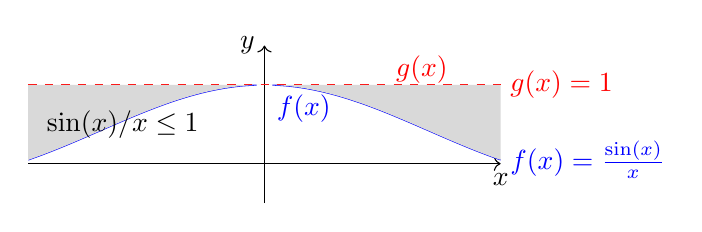
\begin{tikzpicture}
% Axis
\draw[->] (-3,0) -- (3,0) node[below] {$x$};
\draw[->] (0,-0.5) -- (0,1.5) node[left] {$y$};

% Function f(x)
% Splitting the domain to avoid x = 0
\draw[domain=-3:-0.1,smooth,variable=\x,blue] plot ({\x},{sin(deg(\x))/\x});
\draw[domain=0.1:3,smooth,variable=\x,blue] plot ({\x},{sin(deg(\x))/\x}) node[right] {$f(x) = \frac{\sin(x)}{x}$};

% Function g(x)
\draw[dashed,red] (-3,1) -- (3,1) node[right] {$g(x) = 1$};

% Fill
% Adjusting the fill to avoid x = 0
\fill[gray!30] (-3,1) -- plot[domain=-3:-0.1,smooth,variable=\x] ({\x},{sin(deg(\x))/\x}) -- (-0.1,1) -- (0.1,1) -- plot[domain=0.1:3,smooth,variable=\x] ({\x},{sin(deg(\x))/\x}) -- (3,1) -- cycle;

% Labels
\draw (0.5,0.7) node[blue] {$f(x)$};
\draw (2,1.2) node[red] {$g(x)$};
\draw (-1.8,0.5) node {$\sin(x)/x \leq 1$};
\end{tikzpicture}
\end{center}


As shown in the graph, for all \( x \neq 0 \), \( f(x) = \frac{\sin(x)}{x} \) is bounded between -1 and 1. Additionally, \( \lim_{{x \to 0}} \frac{\sin(x)}{x} = 1 \) as it is a well-known limit.

Therefore, by the Squeeze Theorem, since \( -1 \leq \frac{\sin(x)}{x} \leq 1 \) for all \( x \neq 0 \) and \( \lim_{{x \to 0}} \frac{\sin(x)}{x} = 1 \), we conclude that \( \lim_{{x \to 0}} 1 = 1 \).

So, \( \lim_{{x \to 0}} g(x) = 1 \).
\end{example}

The Squeeze Theorem provides a powerful method to evaluate limits by establishing upper and lower bounds for a function and leveraging known limits of the bounding functions.

\subsubsection*{Practice Problems}

Let's practice using the Squeeze Theorem to evaluate limits.

\begin{problem}
Evaluate the following limit using the Squeeze Theorem:
\[
\lim_{{x \to 0}} x^2\sin\left(\frac{1}{x}\right)
\]
\end{problem}

\begin{problem}
Find the limit as \( x \) approaches 0 for the function \( f(x) \) defined as follows:
\[
f(x) =
\begin{cases}
  x & \text{if } x \neq 0 \\
  0 & \text{if } x = 0
\end{cases}
\]
\end{problem}

\begin{problem}
Evaluate the following limit:
\[
\lim_{{x \to 0}} \left(\cos^2(x) + \sin^2(x)\right)
\]
\end{problem}

\begin{problem}
Determine the limit as \( x \) approaches 0 for the function \( g(x) \) defined as follows:
\[
g(x) =
\begin{cases}
  \frac{\sin(x)}{x} & \text{if } x \neq 0 \\
  1 & \text{if } x = 0
\end{cases}
\]
\end{problem}

\subsubsection*{Practice Problems - Solutions}

Let's go through the solutions and explanations for the practice problems.

\begin{problem}
Evaluate the following limit using the Squeeze Theorem:
\[
\lim_{{x \to 0}} x^2\sin\left(\frac{1}{x}\right)
\]
\end{problem}

\begin{solution}
To evaluate this limit, let's use the Squeeze Theorem. First, notice that for all \(x \neq 0\), we have \(-x^2 \leq x^2\sin\left(\frac{1}{x}\right) \leq x^2\). Therefore, we can use the following inequalities:
\[
-x^2 \leq x^2\sin\left(\frac{1}{x}\right) \leq x^2
\]
Next, consider the limits of the bounds as \(x\) approaches 0:
\[
\lim_{{x \to 0}} (-x^2) = 0 \quad \text{and} \quad \lim_{{x \to 0}} (x^2) = 0
\]
Since both \(x^2\) and \(-x^2\) approach 0 as \(x\) approaches 0, we have:
\[
0 \leq \lim_{{x \to 0}} x^2\sin\left(\frac{1}{x}\right) \leq 0
\]
By the Squeeze Theorem, the limit of \(x^2\sin\left(\frac{1}{x}\right)\) as \(x\) approaches 0 is 0.
\end{solution}

\begin{problem}
Find the limit as \(x\) approaches 0 for the function \(f(x)\) defined as follows:
\[
f(x) =
\begin{cases}
  x & \text{if } x \neq 0 \\
  0 & \text{if } x = 0
\end{cases}
\]
\end{problem}

\begin{solution}
To find this limit, we can use the Squeeze Theorem. Consider the function \(f(x) = x\). We know that \(\lim_{{x \to 0}} x = 0\). 

Now, let's analyze the function \(g(x)\) defined as \(g(x) = 0\) for all \(x\). Clearly, \(\lim_{{x \to 0}} g(x) = 0\).

Since \(0 \leq f(x) \leq |x|\) for all \(x\), and both \(f(x)\) and \(|x|\) approach 0 as \(x\) approaches 0, we can apply the Squeeze Theorem to conclude that:
\[
\lim_{{x \to 0}} f(x) = 0
\]
\end{solution}

\begin{problem}
Evaluate the following limit:
\[
\lim_{{x \to 0}} \left(\cos^2(x) + \sin^2(x)\right)
\]
\end{problem}

\begin{solution}
This limit is straightforward to evaluate. Notice that \(\cos^2(x) + \sin^2(x)\) is the identity for all \(x\). Therefore:
\[
\lim_{{x \to 0}} \left(\cos^2(x) + \sin^2(x)\right) = \lim_{{x \to 0}} 1 = 1
\]
\end{solution}

\begin{problem}
Determine the limit as \(x\) approaches 0 for the function \(g(x)\) defined as follows:
\[
g(x) =
\begin{cases}
  \frac{\sin(x)}{x} & \text{if } x \neq 0 \\
  1 & \text{if } x = 0
\end{cases}
\]
\end{problem}

\begin{solution}
To find this limit, we can use the Squeeze Theorem. Consider the function \(f(x) = \frac{\sin(x)}{x}\). We know that \(\lim_{{x \to 0}} \frac{\sin(x)}{x} = 1\) as it is a well-known limit.

Now, let's analyze the function \(h(x)\) defined as \(h(x) = 1\) for all \(x\). Clearly, \(\lim_{{x \to 0}} h(x) = 1\).

Since \(1 \leq f(x) \leq h(x)\) for all \(x\), and both \(f(x)\) and \(h(x)\) approach 1 as \(x\) approaches 0, we can apply the Squeeze Theorem to conclude that:
\[
\lim_{{x \to 0}} \frac{\sin(x)}{x} = 1
\]
\end{solution}


\subsection{Limits of Trigonometric Functions}

In calculus, we often encounter limits involving trigonometric functions. These limits are essential for understanding the behavior of functions near specific points and are used in various mathematical and scientific applications. Let's explore some important limits of trigonometric functions.

\begin{theorem}
One of the fundamental limits involving trigonometric functions is:
\[
\lim_{{x \to 0}} \frac{\sin x}{x} = 1
\]
\end{theorem}

The limit \( \lim_{{x \to 0}} \frac{\sin x}{x} = 1 \) is a crucial result and has significant implications in calculus. It's often referred to as the Sine Limit or Squeeze Theorem. To understand why this limit is equal to 1, let's consider a graphical representation.

\begin{center}
\begin{tikzpicture}
  \begin{axis}[
    axis lines = center,
    xlabel = \(x\),
    ylabel = \(f(x)\),
    xmin = -3, xmax = 3,
    ymin = -0.5, ymax = 1.5,
    unbounded coords=jump, % Skip over problematic points
  ]

  % Function f(x)
  \addplot [
    domain=-3:3,
    samples=200,
    color=blue,
    restrict y to domain=-10:10, % Restrict the y-range to avoid huge values
  ] 
  {sin(deg(\x))/\x};
  \addlegendentry{\(\frac{\sin x}{x}\)}

  % Point at x = 0
  \addplot [mark=*, color=blue] coordinates {(0,1)};

  \end{axis}
\end{tikzpicture}
\end{center}



As \(x\) approaches 0, the graph of \(y = \frac{\sin x}{x}\) approaches the horizontal line \(y = 1\). This visual representation helps illustrate why \( \lim_{{x \to 0}} \frac{\sin x}{x} = 1 \).

The significance of this limit is profound, as it forms the basis for understanding the derivatives of trigonometric functions and plays a crucial role in calculus and mathematical analysis. It is often used as a building block for solving more complex limits involving trigonometric functions.

In addition to the limit mentioned above, there are other important limits involving trigonometric functions that are used in calculus, such as limits involving \(\sin x\), \(\cos x\), and \(\tan x\) as \(x\) approaches specific values. These limits provide insights into the behavior of trigonometric functions near certain points and are essential tools in calculus and mathematics.

In practice, these limits are applied to solve various real-world problems, including physics, engineering, and mathematical modeling. Understanding the limits of trigonometric functions is a fundamental skill for students and professionals in these fields.

\subsubsection*{Practice Problems}

Let's practice evaluating limits of trigonometric functions.

\begin{problem}
Evaluate the following limit:
\[
\lim_{{x \to 0}} \frac{\sin 2x}{x}
\]
\end{problem}

\begin{problem}
Find the limit as \(x\) approaches \(0\) for the function \(f(x)\) defined as:
\[
f(x) =
\begin{cases}
  \frac{\sin 3x}{x} & \text{if } x \neq 0 \\
  0 & \text{if } x = 0
\end{cases}
\]
\end{problem}

\begin{problem}
Determine the limit as \(x\) approaches \(\frac{\pi}{2}\) for the function \(g(x)\) given by:
\[
g(x) = \cos x
\]
\end{problem}

\begin{problem}
Evaluate the following limit:
\[
\lim_{{x \to \frac{\pi}{4}}} \frac{\sin x - \cos x}{x - \frac{\pi}{4}}
\]
\end{problem}

\subsubsection*{Practice Problems - Solutions}

Let's go through the solutions and explanations for the practice problems.

\begin{problem}
Evaluate the following limit:
\[
\lim_{{x \to 0}} \frac{\sin 2x}{x}
\]
\end{problem}

\begin{solution}
To evaluate this limit, we can use the Squeeze Theorem. Notice that for all \(x \neq 0\), we have \(2x \leq \sin 2x \leq 2x\). Therefore, we can use the following inequalities:
\[
2x \leq \frac{\sin 2x}{x} \leq 2x
\]
Next, consider the limits of the bounds as \(x\) approaches 0:
\[
\lim_{{x \to 0}} (2x) = 0
\]
Since both \(2x\) and \(-2x\) approach 0 as \(x\) approaches 0, we have:
\[
0 \leq \lim_{{x \to 0}} \frac{\sin 2x}{x} \leq 0
\]
By the Squeeze Theorem, the limit of \(\frac{\sin 2x}{x}\) as \(x\) approaches 0 is 0.
\end{solution}

\begin{problem}
Find the limit as \(x\) approaches \(0\) for the function \(f(x)\) defined as:
\[
f(x) =
\begin{cases}
  \frac{\sin 3x}{x} & \text{if } x \neq 0 \\
  0 & \text{if } x = 0
\end{cases}
\]
\end{problem}

\begin{solution}
To find this limit, we can directly apply the Sine Limit:
\[
\lim_{{x \to 0}} \frac{\sin x}{x} = 1
\]
In this case, \(3x\) is used instead of \(x\), but the form remains the same. Therefore:
\[
\lim_{{x \to 0}} \frac{\sin 3x}{3x} = \frac{1}{3} \cdot 3 = 1
\]
So, the limit of \(f(x)\) as \(x\) approaches 0 is 1.
\end{solution}

\begin{problem}
Determine the limit as \(x\) approaches \(\frac{\pi}{2}\) for the function \(g(x)\) given by:
\[
g(x) = \cos x
\]
\end{problem}

\begin{solution}
To find this limit, we can directly substitute \(\frac{\pi}{2}\) into the function:
\[
\lim_{{x \to \frac{\pi}{2}}} \cos x = \cos \left(\frac{\pi}{2}\right) = 0
\]
So, the limit of \(g(x)\) as \(x\) approaches \(\frac{\pi}{2}\) is 0.
\end{solution}

\begin{problem}
Evaluate the following limit:
\[
\lim_{{x \to \frac{\pi}{4}}} \frac{\sin x - \cos x}{x - \frac{\pi}{4}}
\]
\end{problem}

\begin{solution}
To evaluate this limit, we can apply L'Hôpital's Rule, as the limit has the form \(\frac{0}{0}\). Taking the derivatives of the numerator and denominator:
\[
\lim_{{x \to \frac{\pi}{4}}} \frac{\frac{d}{dx}(\sin x - \cos x)}{\frac{d}{dx}(x - \frac{\pi}{4})} = \lim_{{x \to \frac{\pi}{4}}} \frac{(\cos x + \sin x)'}{1} = \frac{(\cos \frac{\pi}{4} + \sin \frac{\pi}{4})'}{1} = \frac{\left(\frac{1}{\sqrt{2}} + \frac{1}{\sqrt{2}}\right)}{1} = 1
\]
So, the limit of \(\frac{\sin x - \cos x}{x - \frac{\pi}{4}}\) as \(x\) approaches \(\frac{\pi}{4}\) is 1.
\end{solution}

\section{Continuity - Detail}
\subsection{Continuity Definition and Examples}

In calculus, the concept of continuity is fundamental in understanding the behavior of functions. A function is considered continuous at a point if it satisfies the following criteria:

\begin{definition}
A function is continuous at a point \(x = a\) if the following conditions hold:
\begin{enumerate}
  \item The function is defined at \(x = a\), meaning that \(f(a)\) is defined.
  \item The limit of the function as \(x\) approaches \(a\) exists, denoted as \(\lim_{{x \to a}} f(x)\).
  \item The limit \(\lim_{{x \to a}} f(x)\) is equal to the function value at \(x = a\), i.e., \(\lim_{{x \to a}} f(x) = f(a)\).
\end{enumerate}
\end{definition}

The concept of continuity is crucial because it helps us determine when a function behaves smoothly without abrupt jumps or breaks. Let's explore some examples to illustrate continuity:

\begin{example}
Consider the function \(f(x) = x^2\). Is this function continuous at \(x = 2\)?
\end{example}

\begin{solution}
To check for continuity, we need to verify the three conditions of continuity.

\begin{enumerate}
  \item \(f(2) = 2^2 = 4\), so the function is defined at \(x = 2\).
  \item Next, we find the limit as \(x\) approaches 2:
  \[
  \lim_{{x \to 2}} f(x) = \lim_{{x \to 2}} x^2 = 2^2 = 4
  \]
  The limit exists and is equal to 4.
  \item Since \(f(2) = 4\) and \(\lim_{{x \to 2}} f(x) = 4\), the limit equals the function value at \(x = 2\), and therefore, the function \(f(x) = x^2\) is continuous at \(x = 2\).
\end{enumerate}
\end{solution}

\begin{example}
Now, let's consider the function \(g(x) = \frac{1}{x}\). Is this function continuous at \(x = 0\)?
\end{example}

\begin{solution}
To check for continuity, we again examine the three conditions.

\begin{enumerate}
  \item \(g(0)\) is undefined since division by zero is undefined. Therefore, the function is not defined at \(x = 0\).
  \item We cannot compute the limit as \(x\) approaches 0 for \(g(x)\) since it's undefined at that point.
  \item Since the function is not defined at \(x = 0\), we cannot compare the limit and the function value. Therefore, the function \(g(x) = \frac{1}{x}\) is not continuous at \(x = 0\).
\end{enumerate}
\end{solution}

\begin{example}
Let's consider a piecewise function:
\[
h(x) =
\begin{cases}
  x + 2 & \text{if } x < 1 \\
  3x - 1 & \text{if } x \geq 1
\end{cases}
\]
Is this function continuous at \(x = 1\)?
\end{example}

\begin{solution}
To determine continuity, we examine the three conditions for both branches of the piecewise function separately.

For \(x < 1\):
\begin{enumerate}
  \item \(h(x) = x + 2\), so it is defined at \(x = 1\).
  \item The limit as \(x\) approaches 1 for this branch:
  \[
  \lim_{{x \to 1^-}} (x + 2) = 1 + 2 = 3
  \]
  The limit exists and is equal to 3.
  \item \(h(1) = 1 + 2 = 3\).
\end{enumerate}

For \(x \geq 1\):
\begin{enumerate}
  \item \(h(x) = 3x - 1\), so it is defined at \(x = 1\).
  \item The limit as \(x\) approaches 1 for this branch:
  \[
  \lim_{{x \to 1^+}} (3x - 1) = 3(1) - 1 = 2
  \]
  The limit exists and is equal to 2.
  \item \(h(1) = 3(1) - 1 = 2\).
\end{enumerate}

Since both branches are defined and the limits equal the function values at \(x = 1\), the function \(h(x)\) is continuous at \(x = 1\).
\end{solution}

Continuity is a fundamental concept in calculus, and understanding when a function is continuous at a point helps us analyze and work with functions in various applications.

\subsubsection*{Practice Problems}

Let's practice applying the concept of continuity with some example problems:

\begin{problem}
Determine if the following function is continuous at \(x = 3\):
\[
f(x) =
\begin{cases}
  2x + 1 & \text{if } x < 3 \\
  x^2 - 1 & \text{if } x \geq 3
\end{cases}
\]
\end{problem}

\begin{problem}
Find the values of \(a\) for which the function \(g(x) = ax^2 + 1\) is continuous at \(x = 2\).
\end{problem}

\begin{problem}
Consider the function \(h(x) = \frac{1}{x}\). Determine all the values of \(x\) for which \(h(x)\) is continuous.
\end{problem}

\begin{problem}
Investigate the continuity of the function \(k(x)\) defined as:
\[
k(x) =
\begin{cases}
  \sin x & \text{if } x \neq \pi \\
  0 & \text{if } x = \pi
\end{cases}
\]
\end{problem}

\subsubsection*{Practice Problems - Solutions}

Let's go through the solutions and explanations for the practice problems on continuity.

\begin{problem}
Determine if the following function is continuous at \(x = 3\):
\[
f(x) =
\begin{cases}
  2x + 1 & \text{if } x < 3 \\
  x^2 - 1 & \text{if } x \geq 3
\end{cases}
\]
\end{problem}

\begin{solution}
To check for continuity at \(x = 3\), we need to examine both branches of the function separately.

For \(x < 3\):
\begin{enumerate}
  \item \(f(x) = 2x + 1\), so it is defined at \(x = 3\).
  \item The limit as \(x\) approaches 3 for this branch:
  \[
  \lim_{{x \to 3^-}} (2x + 1) = 2(3) + 1 = 7
  \]
  The limit exists and is equal to 7.
  \item \(f(3) = 2(3) + 1 = 7\).
\end{enumerate}

For \(x \geq 3\):
\begin{enumerate}
  \item \(f(x) = x^2 - 1\), so it is defined at \(x = 3\).
  \item The limit as \(x\) approaches 3 for this branch:
  \[
  \lim_{{x \to 3^+}} (x^2 - 1) = 3^2 - 1 = 8
  \]
  The limit exists and is equal to 8.
  \item \(f(3) = 3^2 - 1 = 8\).
\end{enumerate}

Since both branches are defined and the limits equal the function values at \(x = 3\), the function \(f(x)\) is continuous at \(x = 3\).
\end{solution}

\begin{problem}
Find the values of \(a\) for which the function \(g(x) = ax^2 + 1\) is continuous at \(x = 2\).
\end{problem}

\begin{solution}
For the function \(g(x) = ax^2 + 1\) to be continuous at \(x = 2\), it must satisfy the three conditions of continuity:

\begin{enumerate}
  \item \(g(2) = a(2)^2 + 1 = 4a + 1\) must be defined.
  \item The limit as \(x\) approaches 2, denoted as \(\lim_{{x \to 2}} g(x)\), must exist.
  \item \(\lim_{{x \to 2}} g(x)\) must be equal to \(g(2)\).
\end{enumerate}

First, we consider the limit:
\[
\lim_{{x \to 2}} g(x) = \lim_{{x \to 2}} (ax^2 + 1) = 4a + 1
\]

For the function to be continuous at \(x = 2\), the limit must exist, and it must be equal to \(g(2)\). Therefore, we have:
\[
4a + 1 = 4a + 1
\]

No matter the value of \(a\), the function \(g(x)\) will be continuous at \(x = 2\) since the limit always exists and is equal to \(4a + 1\). So, there are no restrictions on the value of \(a\) for continuity at \(x = 2\).
\end{solution}

\begin{problem}
Consider the function \(h(x) = \frac{1}{x}\). Determine all the values of \(x\) for which \(h(x)\) is continuous.
\end{problem}

\begin{solution}
To find the values of \(x\) for which \(h(x)\) is continuous, we need to consider where the function is defined and check if the limit as \(x\) approaches each point exists.

The function \(h(x) = \frac{1}{x}\) is defined for all \(x\) except when \(x = 0\) since division by zero is undefined. Therefore, \(h(x)\) is not continuous at \(x = 0\) because it's not even defined at that point.

For all other values of \(x\), \(h(x)\) is continuous since it's defined, and the limit as \(x\) approaches any point \(x = a\) (where \(a \neq 0\)) exists and is equal to \(\frac{1}{a}\).

In summary, \(h(x)\) is continuous for all \(x\) except \(x = 0\).
\end{solution}

\begin{problem}
Investigate the continuity of the function \(k(x)\) defined as:
\[
k(x) =
\begin{cases}
  \sin x & \text{if } x \neq \pi \\
  0 & \text{if } x = \pi
\end{cases}
\]
\end{problem}

\begin{solution}
To investigate the continuity of \(k(x)\), we need to check the conditions of continuity at \(x = \pi\).

\begin{enumerate}
  \item \(k(\pi) = 0\) is defined.
  \item The limit as \(x\) approaches \(\pi\):
  \[
  \lim_{{x \to \pi}} k(x) = \lim_{{x \to \pi}} \sin x = \sin(\pi) = 0
  \]
  The limit exists and is equal to 0.
  \item \(k(\pi) = 0\).
\end{enumerate}

Therefore, \(k(x)\) is continuous at \(x = \pi\).

For all other values of \(x\), \(k(x)\) is the sine function, which is known to be continuous everywhere.

In conclusion, \(k(x)\) is continuous for all \(x\).
\end{solution}

\subsection{Types of Discontinuities}

In calculus, discontinuities are points where a function behaves in a way that is not continuous, typically due to a sudden change or a point of undefined behavior. Discontinuities can be classified into three main types: removable, jump, and infinite discontinuities.

\begin{definition}
\textbf{Removable Discontinuity:} A removable discontinuity occurs at a point where the function is undefined or has a jump but can be made continuous by redefining the function value at that point.
\end{definition}

Consider the function \(f(x)\) defined as:

\[
f(x) =
\begin{cases}
  \frac{\sin x}{x} & \text{if } x \neq 0 \\
  2 & \text{if } x = 0
\end{cases}
\]


The graph of \(f(x)\) is shown below:

\begin{center}
\begin{tikzpicture}
  \begin{axis}[
    axis lines = center,
    xlabel = \(x\),
    ylabel = \(f(x)\),
    xmin = -5, xmax = 5,
    ymin = -0.5, ymax = 2.5,
    legend style={at={(0.95,0.95)}, anchor=north east}
  ]
  \addplot [
    domain=-5:5,
    samples=200,
    color=blue,
  ]
  {x == 0 ? 1 : sin(deg(x))/x}; % Conditional function definition
  \addlegendentry{\(\frac{\sin x}{x}\)}

  \addplot [
    mark=*,
    color=red,
    only marks,
    mark size=2pt
  ]
  coordinates {(0,1)}; % Point to represent the limit at x = 0
  \addlegendentry{\(f(0) = 1\)}
  \end{axis}
\end{tikzpicture}
\end{center}


At \(x = 0\), the function \(f(x)\) is undefined (division by zero). However, we can redefine \(f(0)\) as 2 to make it continuous at \(x = 0\). This is an example of a removable discontinuity.


\begin{definition}
\textbf{Jump Discontinuity:} A jump discontinuity occurs at a point where there is a sudden jump in the function's values from one side to the other.
\end{definition}

Consider the function \(g(x)\) defined as:

\[
g(x) =
\begin{cases}
  x + 1 & \text{if } x < 0 \\
  x^2 - 1 & \text{if } x \geq 0
\end{cases}
\]

The graph of \(g(x)\) is shown below:

\begin{center}
\begin{tikzpicture}
  \begin{axis}[
    axis lines = center,
    xlabel = \(x\),
    ylabel = \(g(x)\),
    xmin = -2, xmax = 2,
    ymin = -1.5, ymax = 1.5,
    legend style={at={(0.95,0.95)}, anchor=north east}
  ]
  \addplot [
    domain=-2:0, % Exclusive upper bound
    samples=200,
    color=blue,
  ]
  {x + 1};
  \addlegendentry{\(x + 1\)}

  \addplot [
    domain=0:2, % Exclusive lower bound
    samples=200,
    color=blue,
  ]
  {x^2 - 1};
  \addlegendentry{\(x^2 - 1\)}
  \end{axis}
\end{tikzpicture}
\end{center}


At \(x = 0\), there is a sudden jump in the function's values from \(g(0^-) = 1\) to \(g(0^+) = -1\). This is an example of a jump discontinuity.

\begin{definition}
\textbf{Infinite Discontinuity:} An infinite discontinuity occurs at a point where the function approaches positive or negative infinity as \(x\) approaches that point.
\end{definition}

Consider the function \(h(x)\) defined as:

\[
h(x) =
\begin{cases}
  \frac{1}{x} & \text{if } x \neq 0 \\
  0 & \text{if } x = 0
\end{cases}
\]

The graph of \(h(x)\) is shown below:

\begin{center}
\begin{tikzpicture}
  \begin{axis}[
    axis lines = center,
    xlabel = \(x\),
    ylabel = \(h(x)\),
    xmin = -5, xmax = 5,
    ymin = -5, ymax = 5,
    legend style={at={(0.95,0.95)}, anchor=north east}
  ]
  \addplot [
    domain=-5:-0.1, % Avoid getting too close to 0 from the left
    samples=200,
    color=blue,
  ]
  {1/x};
  \addlegendentry{\(\frac{1}{x}\)}

  \addplot [
    domain=0.1:5, % Avoid getting too close to 0 from the right
    samples=200,
    color=blue,
  ]
  {1/x};
  \end{axis}
\end{tikzpicture}
\end{center}


As \(x\) approaches 0 from the left (\(x \to 0^-\)), \(h(x)\) approaches negative infinity (\(h(x) \to -\infty\)), and as \(x\) approaches 0 from the right (\(x \to 0^+\)), \(h(x)\) approaches positive infinity (\(h(x) \to +\infty\)). This is an example of an infinite discontinuity.

\subsubsection*{Example Problems}

\begin{example}
Consider the function \(f(x)\) defined as:

\[
f(x) =
\begin{cases}
  \frac{x^2 - 4}{x - 2} & \text{if } x \neq 2 \\
  k & \text{if } x = 2
\end{cases}
\]

Determine the value of \(k\) that makes \(f(x)\) continuous at \(x = 2\).
\end{example}

\begin{solution}
For \(f(x)\) to be continuous at \(x = 2\), we need to ensure that the limit of \(f(x)\) as \(x\) approaches 2 exists, and it must be equal to the value of \(f(x)\) at \(x = 2\). 

First, let's calculate the limit as \(x\) approaches 2:

\[
\lim_{{x \to 2}} f(x) = \lim_{{x \to 2}} \frac{x^2 - 4}{x - 2}
\]

We can simplify this limit using algebraic manipulation:

\[
\lim_{{x \to 2}} \frac{x^2 - 4}{x - 2} = \lim_{{x \to 2}} \frac{(x + 2)(x - 2)}{x - 2}
\]

Now, we can cancel the common factor \((x - 2)\) from the numerator and denominator:

\[
\lim_{{x \to 2}} (x + 2) = 2 + 2 = 4
\]

So, the limit of \(f(x)\) as \(x\) approaches 2 is 4. To make \(f(x)\) continuous at \(x = 2\), we set \(k\) to be equal to this limit:

\[
k = 4
\]

Therefore, \(f(x)\) is continuous at \(x = 2\) when \(k = 4\).
\end{solution}

\begin{example}
Consider the function \(g(x)\) defined as:

\[
g(x) =
\begin{cases}
  \sqrt{x} & \text{if } x \geq 0 \\
  -\sqrt{-x} & \text{if } x < 0
\end{cases}
\]

Determine the type(s) of discontinuity, if any, at \(x = 0\).
\end{example}

\begin{solution}
To determine the type(s) of discontinuity at \(x = 0\), we need to analyze the behavior of \(g(x)\) as \(x\) approaches 0 from both the left (\(x \to 0^-\)) and the right (\(x \to 0^+\)).

As \(x\) approaches 0 from the left (\(x \to 0^-\)), \(g(x)\) approaches:

\[
\lim_{{x \to 0^-}} g(x) = \lim_{{x \to 0^-}} (-\sqrt{-x}) = -\sqrt{0} = 0
\]

As \(x\) approaches 0 from the right (\(x \to 0^+\)), \(g(x)\) approaches:

\[
\lim_{{x \to 0^+}} g(x) = \lim_{{x \to 0^+}} (\sqrt{x}) = \sqrt{0} = 0
\]

Both the left and right limits are equal and finite (\(0\)). Therefore, there is no jump or infinite discontinuity at \(x = 0\). However, \(g(x)\) is defined differently for \(x \geq 0\) and \(x < 0\), which means there is a removable discontinuity at \(x = 0\).

To make \(g(x)\) continuous at \(x = 0\), we can redefine the function value at \(x = 0\) as \(g(0) = 0\). This removes the discontinuity, making \(g(x)\) continuous at \(x = 0\).
\end{solution}

\begin{example}
Consider the function \(h(x)\) defined as:

\[
h(x) =
\begin{cases}
  \frac{1}{x^2} & \text{if } x \neq 0 \\
  k & \text{if } x = 0
\end{cases}
\]

Determine the values of \(k\) that make \(h(x)\) continuous at \(x = 0\).
\end{example}

\begin{solution}
For \(h(x)\) to be continuous at \(x = 0\), we need to ensure that the limit of \(h(x)\) as \(x\) approaches 0 exists, and it must be equal to the value of \(h(x)\) at \(x = 0\).

First, let's calculate the limit as \(x\) approaches 0:

\[
\lim_{{x \to 0}} h(x) = \lim_{{x \to 0}} \frac{1}{x^2}
\]

As \(x\) approaches 0, the denominator \(x^2\) approaches 0, and the fraction \(\frac{1}{x^2}\) approaches positive infinity (\(+\infty\)). Therefore, the limit of \(h(x)\) as \(x\) approaches 0 is \(+\infty\).

To make \(h(x)\) continuous at \(x = 0\), we set \(k\) to be equal to this limit:

\[
k = +\infty
\]

Therefore, \(h(x)\) is continuous at \(x = 0\) when \(k = +\infty\).
\end{solution}

\subsubsection*{Solutions to Example Problems}

\begin{example}
Consider the function \(f(x)\) defined as:

\[
f(x) =
\begin{cases}
  \frac{x^2 - 4}{x - 2} & \text{if } x \neq 2 \\
  k & \text{if } x = 2
\end{cases}
\]

Determine the value of \(k\) that makes \(f(x)\) continuous at \(x = 2\).
\end{example}

\begin{solution}
For \(f(x)\) to be continuous at \(x = 2\), we need to ensure that the limit of \(f(x)\) as \(x\) approaches 2 exists, and it must be equal to the value of \(f(x)\) at \(x = 2\). 

First, let's calculate the limit as \(x\) approaches 2:

\[
\lim_{{x \to 2}} f(x) = \lim_{{x \to 2}} \frac{x^2 - 4}{x - 2}
\]

We can simplify this limit using algebraic manipulation:

\[
\lim_{{x \to 2}} \frac{x^2 - 4}{x - 2} = \lim_{{x \to 2}} \frac{(x + 2)(x - 2)}{x - 2}
\]

Now, we can cancel the common factor \((x - 2)\) from the numerator and denominator:

\[
\lim_{{x \to 2}} (x + 2) = 2 + 2 = 4
\]

So, the limit of \(f(x)\) as \(x\) approaches 2 is 4. To make \(f(x)\) continuous at \(x = 2\), we set \(k\) to be equal to this limit:

\[
k = 4
\]

Therefore, \(f(x)\) is continuous at \(x = 2\) when \(k = 4\).
\end{solution}

\begin{example}
Consider the function \(g(x)\) defined as:

\[
g(x) =
\begin{cases}
  \sqrt{x} & \text{if } x \geq 0 \\
  -\sqrt{-x} & \text{if } x < 0
\end{cases}
\]

Determine the type(s) of discontinuity, if any, at \(x = 0\).
\end{example}

\begin{solution}
To determine the type(s) of discontinuity at \(x = 0\), we need to analyze the behavior of \(g(x)\) as \(x\) approaches 0 from both the left (\(x \to 0^-\)) and the right (\(x \to 0^+\)).

As \(x\) approaches 0 from the left (\(x \to 0^-\)), \(g(x)\) approaches:

\[
\lim_{{x \to 0^-}} g(x) = \lim_{{x \to 0^-}} (-\sqrt{-x}) = -\sqrt{0} = 0
\]

As \(x\) approaches 0 from the right (\(x \to 0^+\)), \(g(x)\) approaches:

\[
\lim_{{x \to 0^+}} g(x) = \lim_{{x \to 0^+}} (\sqrt{x}) = \sqrt{0} = 0
\]

Both the left and right limits are equal and finite (\(0\)). Therefore, there is no jump or infinite discontinuity at \(x = 0\). However, \(g(x)\) is defined differently for \(x \geq 0\) and \(x < 0\), which means there is a removable discontinuity at \(x = 0\).

To make \(g(x)\) continuous at \(x = 0\), we can redefine the function value at \(x = 0\) as \(g(0) = 0\). This removes the discontinuity, making \(g(x)\) continuous at \(x = 0\).
\end{solution}

\begin{example}
Consider the function \(h(x)\) defined as:

\[
h(x) =
\begin{cases}
  \frac{1}{x^2} & \text{if } x \neq 0 \\
  k & \text{if } x = 0
\end{cases}
\]

Determine the values of \(k\) that make \(h(x)\) continuous at \(x = 0\).
\end{example}

\begin{solution}
For \(h(x)\) to be continuous at \(x = 0\), we need to ensure that the limit of \(h(x)\) as \(x\) approaches 0 exists, and it must be equal to the value of \(h(x)\) at \(x = 0\).

First, let's calculate the limit as \(x\) approaches 0:

\[
\lim_{{x \to 0}} h(x) = \lim_{{x \to 0}} \frac{1}{x^2}
\]

As \(x\) approaches 0, the denominator \(x^2\) approaches 0, and the fraction \(\frac{1}{x^2}\) approaches positive infinity (\(+\infty\)). Therefore, the limit of \(h(x)\) as \(x\) approaches 0 is \(+\infty\).

To make \(h(x)\) continuous at \(x = 0\), we set \(k\) to be equal to this limit:

\[
k = +\infty
\]

Therefore, \(h(x)\) is continuous at \(x = 0\) when \(k = +\infty\).
\end{solution}

\subsection{Intermediate Value Theorem}

\begin{theorem}
If a function is continuous on a closed interval \([a, b]\) and \( N \) is any number between \( f(a) \) and \( f(b) \), then there exists a number \( c \) in the interval such that \( f(c) = N \).
\end{theorem}

\begin{definition}
A function \( f \) is said to be continuous on a closed interval \([a, b]\) if it is continuous at every point in the interval.
\end{definition}

\begin{discussion}
The Intermediate Value Theorem is a fundamental result in calculus that asserts the existence of a point in a continuous function where the function takes on a given value. This theorem is particularly useful in proving the existence of roots.
\end{discussion}

\begin{example}
Consider the function \( f(x) = x^2 - 4 \) on the interval \([-3, 3]\). Since \( f(-3) = 5 \) and \( f(3) = 5 \), and \( 0 \) is between \( 5 \) and \( 5 \), by the Intermediate Value Theorem, there exists a \( c \) in \([-3, 3]\) such that \( f(c) = 0 \).
\end{example}

\begin{center}
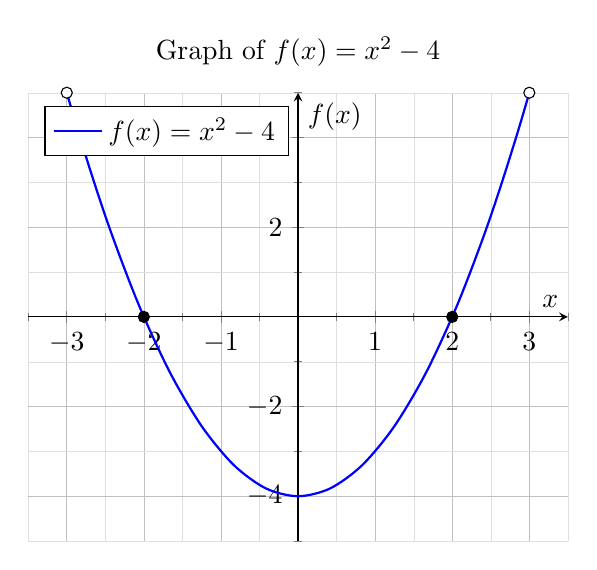
\begin{tikzpicture}
\begin{axis}[
    title={Graph of \( f(x) = x^2 - 4 \)},
    xlabel=\( x \),
    ylabel=\( f(x) \),
    xmin=-3.5, xmax=3.5,
    ymin=-5, ymax=5,
    axis lines=center,
    grid=both,
    minor tick num=1,
    major grid style={line width=.2pt,draw=gray!50},
    minor grid style={line width=.1pt,draw=gray!25},
    legend pos=north west,
]

\addplot[smooth, thick, color=blue] {x^2 - 4};
\addlegendentry{\( f(x) = x^2 - 4 \)}

\addplot[holdot] coordinates{(-2,0) (2,0)};
\addplot[soldot] coordinates{(-3,5) (3,5)};

\end{axis}
\end{tikzpicture}
\end{center}

\begin{exercise}
Show using the Intermediate Value Theorem that the function \( g(x) = x^3 - x - 1 \) has a root in the interval \([1, 2]\).
\end{exercise}

% You may add more exercises, examples, or discussions as needed.

\subsubsection*{Practice Problems on Intermediate Value Theorem}

\begin{problem}
Show that the function \( h(x) = 3x^3 - 2x + 1 \) has at least one root in the interval \([-2, 2]\). 
\end{problem}

\begin{solution}[Optional]
% Here you can include a detailed solution or hints. This part can be left for the students to solve.
\end{solution}

\begin{problem}
Consider the function \( k(x) = \cos(x) - x \). Use the Intermediate Value Theorem to prove that there is a root of \( k \) in the interval \([0, \frac{\pi}{2}]\).
\end{problem}

\begin{solution}[Optional]
% Solution or hints go here.
\end{solution}

\begin{problem}
Let \( f(x) = e^x - 4x \). Demonstrate using the IVT that \( f \) has a root between 1 and 2.
\end{problem}

\begin{solution}[Optional]
% Solution or hints go here.
\end{solution}

\begin{problem}
Given the function \( m(x) = x^5 - 5x + 4 \), use the Intermediate Value Theorem to find an interval of length 1 where \( m \) must have a root.
\end{problem}

\begin{solution}[Optional]
% Solution or hints go here.
\end{solution}

\begin{problem}
Assume the function \( p(x) = \ln(x) - x^2 + 3 \) is continuous on the interval \([1, 4]\). Apply the IVT to prove that \( p \) has at least one root in this interval.
\end{problem}

\begin{solution}[Optional]
% Solution or hints go here.
\end{solution}

% More problems can be added as per the requirement.

\subsubsection*{Solutions to Practice Problems on Intermediate Value Theorem}

\begin{solution}[\textbf{Problem 1}]
To show that \( h(x) = 3x^3 - 2x + 1 \) has at least one root in the interval \([-2, 2]\), we need to check the values of \( h \) at the endpoints and apply the IVT.

At \( x = -2 \), \( h(-2) = 3(-2)^3 - 2(-2) + 1 = -24 + 4 + 1 = -19 \).

At \( x = 2 \), \( h(2) = 3(2)^3 - 2(2) + 1 = 24 - 4 + 1 = 21 \).

Since \( h(-2) < 0 \) and \( h(2) > 0 \), and \( h \) is a polynomial (hence continuous), by the IVT, there is at least one root of \( h \) in the interval \([-2, 2]\).
\end{solution}

\begin{solution}[\textbf{Problem 2}]
For \( k(x) = \cos(x) - x \), we evaluate \( k \) at \( 0 \) and \( \frac{\pi}{2} \):

At \( x = 0 \), \( k(0) = \cos(0) - 0 = 1 \).

At \( x = \frac{\pi}{2} \), \( k(\frac{\pi}{2}) = \cos(\frac{\pi}{2}) - \frac{\pi}{2} = -\frac{\pi}{2} \).

Since \( k(0) > 0 \) and \( k(\frac{\pi}{2}) < 0 \), and \( k \) is continuous, there must be a root of \( k \) in the interval \([0, \frac{\pi}{2}]\) by the IVT.
\end{solution}

\begin{solution}[\textbf{Problem 3}]
To apply the IVT to \( f(x) = e^x - 4x \) in the interval [1, 2], we first evaluate \( f \) at the endpoints:

At \( x = 1 \), \( f(1) = e^1 - 4(1) = e - 4 \).

At \( x = 2 \), \( f(2) = e^2 - 4(2) = e^2 - 8 \).

Since \( e < 4 \) and \( e^2 > 8 \), it follows that \( f(1) < 0 \) and \( f(2) > 0 \). Hence, by the IVT, there is a root of \( f \) between 1 and 2.
\end{solution}

\begin{solution}[\textbf{Problem 4}]
For the function \( m(x) = x^5 - 5x + 4 \), we need to find an interval of length 1 where \( m \) has a root. 

Consider the intervals \([-1, 0]\) and \([0, 1]\). We compute \( m(-1) \), \( m(0) \), and \( m(1) \):

\( m(-1) = (-1)^5 - 5(-1) + 4 = -1 + 5 + 4 = 8 \).

\( m(0) = 0^5 - 5(0) + 4 = 4 \).

\( m(1) = 1^5 - 5(1) + 4 = 0 \).

Since \( m(-1) > 0 \) and \( m(0) < 0 \), there is at least one root in \([-1, 0]\) by the IVT. Similarly, since \( m(0) < 0 \) and \( m(1) = 0 \), there is a root at \( x = 1 \) in \([0, 1]\).
\end{solution}

\begin{solution}[\textbf{Problem 5}]
For \( p(x) = \ln(x) - x^2 + 3 \), evaluate \( p \) at \( x = 1 \) and \( x = 4 \):

\( p(1) = \ln(1) - 1^2 + 3 = 0 - 1 + 3 = 2 \).

\( p(4) = \ln(4) - 4^2 + 3 = \ln(4) - 16 + 3 = \ln(4) - 13 \).

Since \( \ln(4) < 13 \), it follows that \( p(4) < 0 \). Given \( p(1) > 0 \) and \( p(4) < 0 \), and \( p \) is continuous on \([1, 4]\), by the IVT, there is at least one root of \( p \) in this interval.
\end{solution}

% End of solutions

\chapter{The Derivative - Detail}
\section{Understanding Derivatives}
\subsection{Derivative Definition and Notation}

\begin{definition}
The derivative of a function \( f \) at a point \( a \) is defined as \(\lim_{h \to 0} \frac{f(a+h) - f(a)}{h}\), if this limit exists. This derivative is denoted as \( f'(a) \) or \( \frac{df}{dx}(a) \).
\end{definition}

The derivative of a function at a point is a fundamental concept in calculus. It represents the rate at which the function's value changes at that point. Geometrically, the derivative corresponds to the slope of the tangent line to the function's graph at that point.

\begin{example}[Graphical Representation of Derivative]
Consider the function \( f(x) = x^2 \) and the point \( a = 2 \). The derivative at this point is the slope of the tangent line to the graph of \( f \) at \( x = 2 \).

\begin{center}
\begin{tikzpicture}
    \begin{axis}[
        axis lines = center,
        xlabel = \( x \),
        ylabel = \( y \),
        xmin = 0, xmax = 4,
        ymin = 0, ymax = 5,
        legend style={at={(0.95,0.95)}, anchor=north east}
    ]
    % Plot function
    \addplot [
        domain=0:4,
        samples=100,
        color=blue,
    ] 
    {x^2};
    \addlegendentry{\( f(x) = x^2 \)}

    % Tangent line at x = 2
    \addplot [
        domain=1:3,
        samples=2,
        color=red,
    ] 
    {4*x - 4}; % Tangent line equation
    \addlegendentry{Tangent at \( x = 2 \)}

    % Point at x = 2
    \addplot [holdot] coordinates {(2,4)};
    \node[label={above:\( (2, f(2)) \)},circle,fill,inner sep=2pt] at (axis cs:2,4) {};

    \end{axis}
\end{tikzpicture}
\end{center}

In this case, the slope of the tangent line (the derivative) at \( x = 2 \) can be calculated as:
\[ f'(2) = \lim_{h \to 0} \frac{f(2+h) - f(2)}{h} = \lim_{h \to 0} \frac{(2+h)^2 - 4}{h} = 4. \]
Thus, the derivative of \( f(x) = x^2 \) at \( x = 2 \) is 4.
\end{example}

The concept of the derivative is widely used in various fields of mathematics, physics, engineering, and beyond. It provides a powerful tool for analyzing and understanding how functions behave and change.

\subsubsection*{Exercises on Derivatives}

The following exercises will help solidify your understanding of calculating derivatives. Try to solve them and then check your answers against the provided solutions.

\begin{exercise}
Find the derivative of the function \( f(x) = 3x^3 - 2x^2 + 5x - 7 \) at \( x = 1 \).
\end{exercise}

\begin{solution}
Using the definition of the derivative,
\[ f'(x) = \lim_{h \to 0} \frac{f(x+h) - f(x)}{h} \]
for \( f(x) = 3x^3 - 2x^2 + 5x - 7 \), we find
\[ f'(1) = \lim_{h \to 0} \frac{3(1+h)^3 - 2(1+h)^2 + 5(1+h) - 7 - (3 - 2 + 5 - 7)}{h}. \]
Simplifying and evaluating this limit gives the derivative at \( x = 1 \).
\end{solution}

\begin{exercise}
Determine the slope of the tangent line to the curve \( g(x) = \sqrt{x} \) at \( x = 4 \).
\end{exercise}

\begin{solution}
The slope of the tangent line is given by the derivative of \( g(x) \) at \( x = 4 \). The derivative is
\[ g'(x) = \frac{1}{2\sqrt{x}}. \]
Therefore, the slope at \( x = 4 \) is \( g'(4) = \frac{1}{2\sqrt{4}} = \frac{1}{4}. \)
\end{solution}

\begin{exercise}
Calculate the derivative of \( h(x) = \frac{1}{x^2} \) at any point \( x \).
\end{exercise}

\begin{solution}
The derivative of \( h(x) = \frac{1}{x^2} \) is
\[ h'(x) = \lim_{h \to 0} \frac{\frac{1}{(x+h)^2} - \frac{1}{x^2}}{h}. \]
Simplifying this expression will give the general formula for the derivative of \( h(x) \).
\end{solution}

\begin{exercise}
What is the derivative of the constant function \( k(x) = 17 \)?
\end{exercise}

\begin{solution}
For any constant function \( k(x) = c \), where \( c \) is a constant, the derivative is zero. Hence, \( k'(x) = 0 \).
\end{solution}

These exercises cover a range of fundamental concepts in differentiation. By working through these problems, you'll gain a better understanding of how to compute derivatives and interpret their geometric meaning.

\subsubsection*{Solutions to Exercises on Derivatives}

Here are the detailed solutions and explanations for the exercises on derivatives.

\begin{solution}[to Exercise 1]
To find the derivative of the function \( f(x) = 3x^3 - 2x^2 + 5x - 7 \) at \( x = 1 \), we first calculate the derivative of \( f(x) \) and then evaluate it at \( x = 1 \).

The derivative \( f'(x) \) is calculated using standard differentiation rules:
\[ f'(x) = \frac{d}{dx}(3x^3) - \frac{d}{dx}(2x^2) + \frac{d}{dx}(5x) - \frac{d}{dx}(7) = 9x^2 - 4x + 5. \]

Evaluating this at \( x = 1 \) gives:
\[ f'(1) = 9(1)^2 - 4(1) + 5 = 9 - 4 + 5 = 10. \]

Therefore, the derivative of \( f(x) \) at \( x = 1 \) is \( 10 \).
\end{solution}

\begin{solution}[to Exercise 2]
The slope of the tangent line to the curve \( g(x) = \sqrt{x} \) at \( x = 4 \) is given by \( g'(4) \).

First, find the derivative \( g'(x) \):
\[ g'(x) = \frac{d}{dx}(\sqrt{x}) = \frac{1}{2\sqrt{x}}. \]

Now, evaluate \( g'(x) \) at \( x = 4 \):
\[ g'(4) = \frac{1}{2\sqrt{4}} = \frac{1}{4}. \]

The slope of the tangent line at \( x = 4 \) is \( \frac{1}{4} \).
\end{solution}

\begin{solution}[to Exercise 3]
To calculate the derivative of \( h(x) = \frac{1}{x^2} \) at any point \( x \), we use the power rule for differentiation:

\[ h'(x) = \frac{d}{dx}\left(\frac{1}{x^2}\right) = \frac{d}{dx}(x^{-2}) = -2x^{-3} = -\frac{2}{x^3}. \]

So, the derivative of \( h(x) \) is \( -\frac{2}{x^3} \).
\end{solution}

\begin{solution}[to Exercise 4]
The derivative of a constant function \( k(x) = 17 \) is zero. This is because the rate of change of a constant function is always zero. Hence, \( k'(x) = 0 \).
\end{solution}

These solutions provide a step-by-step approach to understanding and solving basic derivative problems. They demonstrate the application of differentiation rules and the interpretation of derivatives in various contexts.

\subsection{Interpreting Derivatives}

\begin{discussion}
The derivative of a function at a point provides critical information about the behavior of the function at that point. It gives the slope of the tangent line to the function's graph and represents the rate of change of the function with respect to its variable. This can be interpreted in various ways:

\begin{itemize}
    \item \textbf{Slope of Tangent:} The derivative at a point \(a\) gives the slope of the tangent line to the graph of the function at that point. A positive derivative indicates an increasing function, while a negative derivative indicates a decreasing function.
    \item \textbf{Rate of Change:} The derivative is a measure of how fast the function's value is changing at that point. It is especially important in physics for understanding velocity and acceleration.
\end{itemize}
\end{discussion}

\subsection{Graphical Interpretation}
Consider the function \( f(x) = x^2 \). The derivative of \( f \) at a point \( x = a \) is given by \( f'(a) = 2a \). This derivative represents the slope of the tangent line at \( x = a \).

\begin{center}
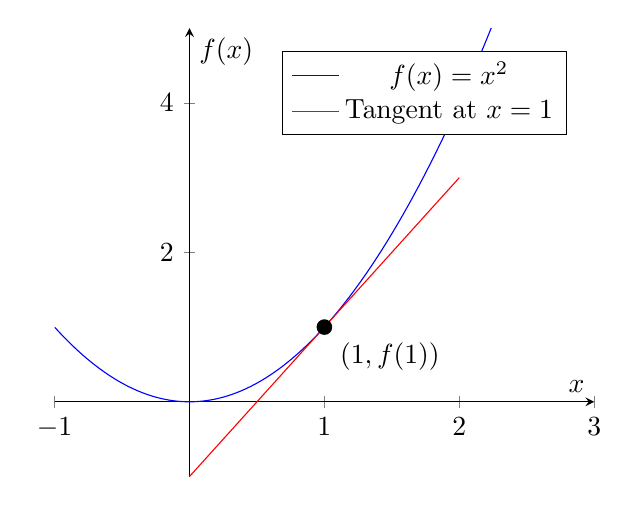
\begin{tikzpicture}
    \begin{axis}[
        axis lines = middle,
        xlabel = \(x\),
        ylabel = \(f(x)\),
        xmin = -1, xmax = 3,
        ymin = -1, ymax = 5,
        legend style={at={(0.95,0.95)}, anchor=north east}
    ]
    % Function f(x)
    \addplot [
        domain=-1:3,
        samples=100,
        color=blue,
    ] 
    {x^2};
    \addlegendentry{\(f(x) = x^2\)}

    % Tangent line at x = 1
    \addplot [
        domain=0:2,
        samples=2,
        color=red,
    ] 
    {2*x - 1}; % y = f'(1)(x - 1) + f(1)
    \addlegendentry{Tangent at \(x = 1\)}

    % Point at x = 1
    \addplot[holdot] coordinates {(1,1)};
    \node[label={below right:\( (1, f(1)) \)},circle,fill,inner sep=2pt] at (axis cs:1,1) {};

    \end{axis}
\end{tikzpicture}
\end{center}

In this graph, the tangent line at \( x = 1 \) has a slope of \( f'(1) = 2 \), illustrating how the derivative provides the slope at a specific point on the curve.

\subsection{Practical Implications}
Understanding derivatives is crucial in many scientific and engineering fields. For instance, in physics, the derivative of position with respect to time gives the velocity, and the derivative of velocity gives acceleration. In economics, the derivative can represent the rate of change in cost or revenue.

Interpreting derivatives thus provides a powerful tool for analyzing and predicting the behavior of various phenomena described mathematically.

\subsubsection*{Exercises on Interpreting Derivatives}

The following exercises are designed to help you apply and deepen your understanding of derivatives.

\begin{exercise}
Given the function \( f(x) = x^3 - 3x^2 + 5 \), find the slope of the tangent line to the graph of \( f \) at \( x = 2 \).
\end{exercise}

\begin{exercise}
Consider the function \( g(x) = \frac{1}{x} \). Determine where the function is increasing and decreasing.
\end{exercise}

\begin{exercise}
A particle moves along a line with its position at time \( t \) given by \( s(t) = 2t^2 - 3t + 1 \). Find the velocity of the particle at \( t = 4 \).
\end{exercise}

\begin{exercise}
Find the points on the curve \( y = x^4 - 4x^3 \) where the tangent is horizontal.
\end{exercise}

\subsection{Solutions to Exercises on Interpreting Derivatives}

\begin{solution}[to Exercise 1]
First, find the derivative \( f'(x) \) of \( f(x) = x^3 - 3x^2 + 5 \):
\[ f'(x) = 3x^2 - 6x. \]
Then, find the slope of the tangent line at \( x = 2 \):
\[ f'(2) = 3(2)^2 - 6(2) = 12 - 12 = 0. \]
The slope of the tangent line at \( x = 2 \) is \( 0 \).
\end{solution}

\begin{solution}[to Exercise 2]
Find the derivative of \( g(x) = \frac{1}{x} \):
\[ g'(x) = -\frac{1}{x^2}. \]
The function is increasing where \( g'(x) > 0 \) and decreasing where \( g'(x) < 0 \). Since \( g'(x) \) is always negative, \( g(x) \) is always decreasing.
\end{solution}

\begin{solution}[to Exercise 3]
The velocity of the particle is the derivative of \( s(t) \):
\[ s'(t) = 4t - 3. \]
The velocity at \( t = 4 \) is:
\[ s'(4) = 4(4) - 3 = 16 - 3 = 13. \]
The velocity at \( t = 4 \) is \( 13 \) units per time interval.
\end{solution}

\begin{solution}[to Exercise 4]
Find \( y' \) and set it equal to \( 0 \) to find points where the tangent is horizontal:
\[ y' = 4x^3 - 12x^2, \]
\[ 0 = 4x^3 - 12x^2. \]
Solving this gives the points where the tangent is horizontal.
\end{solution}

These exercises and solutions explore various aspects of derivatives, from the slope of tangent lines to real-world applications such as motion analysis.

\subsection{Derivative as a Function}

\begin{definition}
The derivative of a function \( f \), denoted as \( f'(x) \) or \( \frac{df}{dx} \), is a function that assigns to each point \( x \) in the domain of \( f \) the slope of the tangent line to the graph of \( f \) at \( x \). This function provides a means to understand how \( f \) changes at each point.
\end{definition}

\subsection{A Derivative's Graphical Interpretation}
Consider a function \( f(x) \) and its derivative \( f'(x) \). The graph of \( f'(x) \) can be understood as a plot of the slopes of the tangents to the graph of \( f(x) \) at each point.

% Example function and its derivative
\example{Let \( f(x) = x^2 \). The derivative function is \( f'(x) = 2x \).}

\begin{center}
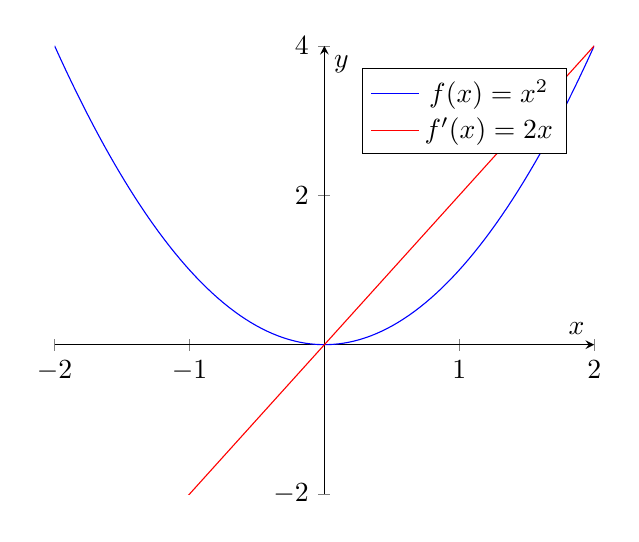
\begin{tikzpicture}
    \begin{axis}[
        axis lines = middle,
        xlabel = \(x\),
        ylabel = \(y\),
        xmin = -2, xmax = 2,
        ymin = -2, ymax = 4,
        legend style={at={(0.95,0.95)}, anchor=north east}
    ]
    % Original function f(x)
    \addplot [
        domain=-2:2,
        samples=100,
        color=blue,
    ] 
    {x^2};
    \addlegendentry{\(f(x) = x^2\)}

    % Derivative function f'(x)
    \addplot [
        domain=-2:2,
        samples=100,
        color=red,
    ] 
    {2*x};
    \addlegendentry{\(f'(x) = 2x\)}

    \end{axis}
\end{tikzpicture}
\end{center}

In this graph, the blue curve represents the function \( f(x) = x^2 \), and the red curve represents its derivative \( f'(x) = 2x \). The derivative graph shows the slope of the tangent to \( f(x) \) at each point \( x \).

\subsection{Significance of the Derivative Function}
The derivative function \( f'(x) \) provides valuable information about the behavior of \( f(x) \):

\begin{itemize}
    \item Where \( f'(x) > 0 \), \( f(x) \) is increasing.
    \item Where \( f'(x) < 0 \), \( f(x) \) is decreasing.
    \item Where \( f'(x) = 0 \), \( f(x) \) may have a local maximum, minimum, or inflection point.
\end{itemize}

Understanding the derivative as a function itself allows for a deeper analysis of the original function, particularly in understanding its growth, decay, and points of extrema.

\subsubsection*{Exercises on Derivative as a Function}

The following exercises are designed to help you apply and deepen your understanding of the derivative as a function.

\begin{exercise}
Find the derivative function \( f'(x) \) for \( f(x) = 3x^3 - 2x + 1 \). Then, determine the intervals where \( f(x) \) is increasing and decreasing.
\end{exercise}

\begin{exercise}
Given the function \( g(x) = \cos(x) \), sketch the graph of \( g \) and its derivative \( g'(x) \) on the same axes. Indicate points of maximum, minimum, and points where the tangent is horizontal.
\end{exercise}

\begin{exercise}
For the function \( h(x) = \frac{1}{x^2} \), compute the derivative \( h'(x) \). Use the derivative to discuss the concavity of the function.
\end{exercise}

\begin{exercise}
Consider \( f(x) = e^x \). Find \( f'(x) \) and describe how the behavior of \( f'(x) \) relates to the behavior of \( f(x) \).
\end{exercise}

\subsection{Solutions to Exercises on Derivative as a Function}

\begin{solution}[to Exercise 1]
The derivative of \( f(x) = 3x^3 - 2x + 1 \) is \( f'(x) = 9x^2 - 2 \). 
To find where \( f(x) \) is increasing or decreasing, determine the sign of \( f'(x) \) for different intervals. \( f(x) \) is increasing where \( f'(x) > 0 \) and decreasing where \( f'(x) < 0 \).
\end{solution}

\begin{solution}[to Exercise 2]
The derivative of \( g(x) = \cos(x) \) is \( g'(x) = -\sin(x) \). Sketching \( g \) and \( g' \) together, you'll notice that \( g'(x) \) is zero at the maxima and minima of \( g(x) \), indicating points where the tangent to \( g(x) \) is horizontal.
\end{solution}

\begin{solution}[to Exercise 3]
The derivative of \( h(x) = \frac{1}{x^2} \) is \( h'(x) = -\frac{2}{x^3} \). The concavity of \( h(x) \) is determined by the sign of \( h'(x) \). Since \( h'(x) \) is always negative, \( h(x) \) is concave down for its entire domain.
\end{solution}

\begin{solution}[to Exercise 4]
The derivative of \( f(x) = e^x \) is \( f'(x) = e^x \), which is the same as \( f(x) \). This means that the rate of change of \( e^x \) is equal to its value at any point, showing an exponential rate of increase.
\end{solution}

These exercises and solutions provide a practical application of the concept of the derivative as a function, enhancing understanding through specific examples.

\section{Techniques of Differentiation}
\subsection{Product Rule and Quotient Rule}
\begin{theorem}
The Product Rule states that for two differentiable functions \( f \) and \( g \), the derivative of their product \( fg \) is given by \( (fg)' = f'g + fg' \). The Quotient Rule states that for two differentiable functions \( f \) and \( g \) (with \( g \) not equal to zero), the derivative of their quotient \( \frac{f}{g} \) is given by \( \left(\frac{f}{g}\right)' = \frac{f'g - fg'}{g^2} \).
\end{theorem}

\subsection{Graphical Representation of the Product Rule}
Consider two functions \( f(x) \) and \( g(x) \). The graph below illustrates the product rule by showing \( f(x) \), \( g(x) \), and their product \( f(x)g(x) \) along with their derivatives.

% Example functions
\example{Let \( f(x) = x^2 \) and \( g(x) = e^x \).}

\begin{center}
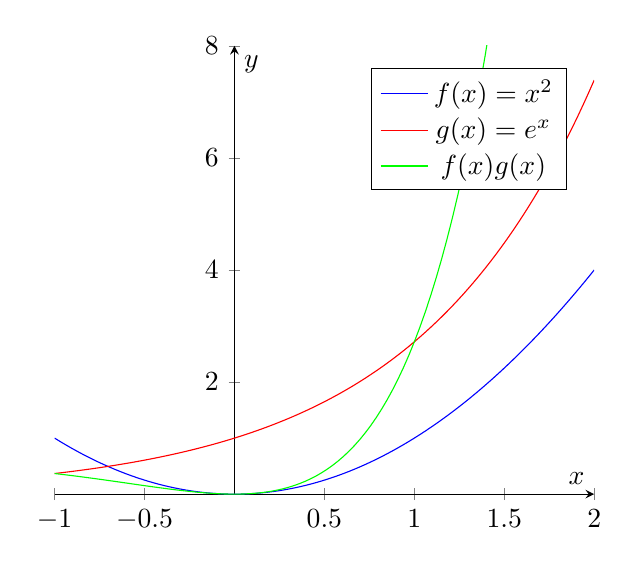
\begin{tikzpicture}
    \begin{axis}[
        axis lines = middle,
        xlabel = \(x\),
        ylabel = \(y\),
        xmin = -1, xmax = 2,
        ymin = 0, ymax = 8,
        legend style={at={(0.95,0.95)}, anchor=north east}
    ]
    % f(x) = x^2
    \addplot [
        domain=-1:2,
        samples=100,
        color=blue,
    ] 
    {x^2};
    \addlegendentry{\(f(x) = x^2\)}

    % g(x) = e^x
    \addplot [
        domain=-1:2,
        samples=100,
        color=red,
    ] 
    {exp(x)};
    \addlegendentry{\(g(x) = e^x\)}

    % Product f(x)g(x)
    \addplot [
        domain=-1:2,
        samples=100,
        color=green,
    ] 
    {exp(x)*x^2};
    \addlegendentry{\(f(x)g(x)\)}

    \end{axis}
\end{tikzpicture}
\end{center}

\subsection{Graphical Representation of the Quotient Rule}
Similarly, for the quotient rule, consider functions \( f(x) \) and \( g(x) \). The graph below illustrates the quotient rule by showing \( f(x) \), \( g(x) \), and their quotient \( \frac{f(x)}{g(x)} \) along with their derivatives.

% Example functions for Quotient Rule
\example{Let \( f(x) = x^3 \) and \( g(x) = x + 1 \).}

\begin{center}
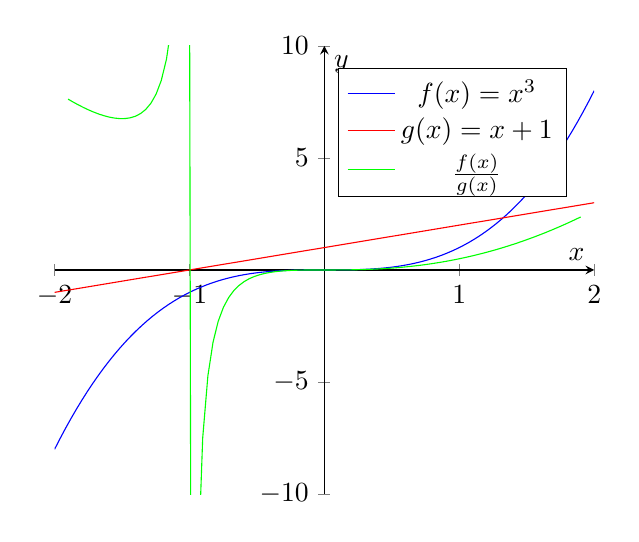
\begin{tikzpicture}
    \begin{axis}[
        axis lines = middle,
        xlabel = \(x\),
        ylabel = \(y\),
        xmin = -2, xmax = 2,
        ymin = -10, ymax = 10,
        legend style={at={(0.95,0.95)}, anchor=north east}
    ]
    % f(x) = x^3
    \addplot [
        domain=-2:2,
        samples=100,
        color=blue,
    ] 
    {x^3};
    \addlegendentry{\(f(x) = x^3\)}

    % g(x) = x + 1
    \addplot [
        domain=-2:2,
        samples=100,
        color=red,
    ] 
    {x + 1};
    \addlegendentry{\(g(x) = x + 1\)}

    % Quotient f(x)/g(x)
    \addplot [
        domain=-1.9:1.9, % Avoid division by zero
        samples=100,
        color=green,
    ] 
    {x^3/(x + 1)};
    \addlegendentry{\(\frac{f(x)}{g(x)}\)}

    \end{axis}
\end{tikzpicture}
\end{center}

These graphical representations help in visualizing how the derivatives of the product and quotient of two functions are related to the derivatives of the individual functions. They also highlight the importance of understanding these rules for effective differentiation of more complex functions.

\subsubsection*{Exercises on Product Rule and Quotient Rule}

The following exercises aim to help you practice and understand the Product Rule and Quotient Rule for differentiation.

\begin{exercise}
Using the Product Rule, find the derivative of \( h(x) = (x^3 + 2x)(\sin x) \).
\end{exercise}

\begin{exercise}
Apply the Quotient Rule to differentiate \( f(x) = \frac{x^2 - 1}{x + 2} \).
\end{exercise}

\begin{exercise}
Given \( g(x) = e^x \cdot \ln x \), use the Product Rule to find \( g'(x) \).
\end{exercise}

\begin{exercise}
Differentiate the function \( k(x) = \frac{\tan x}{x^2 + 1} \) using the Quotient Rule.
\end{exercise}

\subsubsection*{Solutions to Exercises on Product Rule and Quotient Rule}

\begin{solution}[to Exercise 1]
For \( h(x) = (x^3 + 2x)(\sin x) \), we apply the Product Rule:
\[ h'(x) = (x^3 + 2x)' \sin x + (x^3 + 2x) (\sin x)' = (3x^2 + 2)\sin x + (x^3 + 2x)\cos x. \]
\end{solution}

\begin{solution}[to Exercise 2]
For \( f(x) = \frac{x^2 - 1}{x + 2} \), apply the Quotient Rule:
\[ f'(x) = \frac{(x^2 - 1)'(x + 2) - (x^2 - 1)(x + 2)'}{(x + 2)^2} = \frac{2x(x + 2) - (x^2 - 1)}{(x + 2)^2}. \]
\end{solution}

\begin{solution}[to Exercise 3]
For \( g(x) = e^x \cdot \ln x \), the Product Rule gives:
\[ g'(x) = (e^x)' \ln x + e^x (\ln x)' = e^x \ln x + \frac{e^x}{x}. \]
\end{solution}

\begin{solution}[to Exercise 4]
For \( k(x) = \frac{\tan x}{x^2 + 1} \), use the Quotient Rule:
\[ k'(x) = \frac{(\tan x)'(x^2 + 1) - \tan x (x^2 + 1)'}{(x^2 + 1)^2} = \frac{\sec^2 x (x^2 + 1) - 2x \tan x}{(x^2 + 1)^2}. \]
\end{solution}

These exercises provide a practical application of the Product Rule and Quotient Rule in different scenarios, enhancing the understanding of these fundamental differentiation techniques.

\subsection{Chain Rule}

\begin{theorem}
If a function \( y \) is a function of \( u \), which is in turn a function of \( x \), then the derivative of \( y \) with respect to \( x \) is given by the product of the derivatives of \( y \) with respect to \( u \) and \( u \) with respect to \( x \), that is, \( \frac{dy}{dx} = \frac{dy}{du} \cdot \frac{du}{dx} \).
\end{theorem}

\subsubsection*{Application of the Chain Rule}
The Chain Rule is particularly useful when dealing with composite functions, where one function is nested within another.

\example{Consider \( y = \sin(u) \) and \( u = x^2 + 1 \). We want to find \( \frac{dy}{dx} \).}

Applying the Chain Rule, we have:
\[ \frac{dy}{dx} = \frac{dy}{du} \cdot \frac{du}{dx} = \cos(u) \cdot 2x = \cos(x^2 + 1) \cdot 2x. \]

\subsection{Chain Rule Graphical Representation}
To visualize the Chain Rule, we can plot both the inner function \( u(x) = x^2 + 1 \) and the composite function \( y(x) = \sin(x^2 + 1) \), along with their derivatives.

\begin{center}
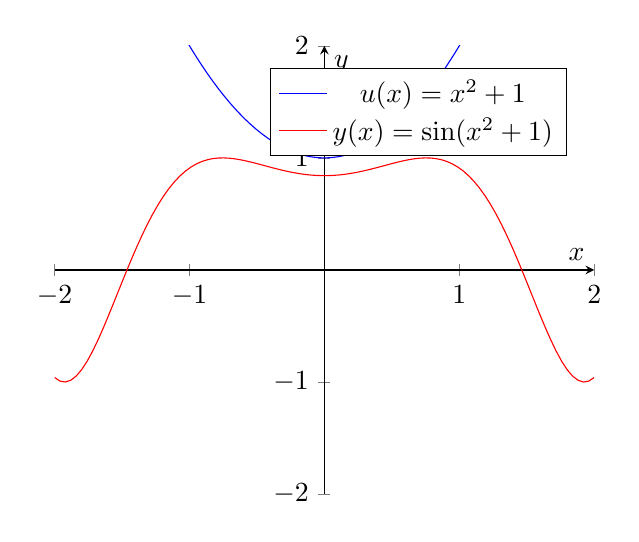
\begin{tikzpicture}
    \begin{axis}[
        axis lines = middle,
        xlabel = \(x\),
        ylabel = \(y\),
        xmin = -2, xmax = 2,
        ymin = -2, ymax = 2,
        legend style={at={(0.95,0.95)}, anchor=north east}
    ]
    % u(x) = x^2 + 1
    \addplot [
        domain=-2:2,
        samples=100,
        color=blue,
    ] 
    {x^2 + 1};
    \addlegendentry{\(u(x) = x^2 + 1\)}

    % y(x) = sin(u(x))
    \addplot [
        domain=-2:2,
        samples=100,
        color=red,
    ] 
    {sin(deg(x^2 + 1))};
    \addlegendentry{\(y(x) = \sin(x^2 + 1)\)}

    \end{axis}
\end{tikzpicture}
\end{center}

This graph shows how the Chain Rule applies to the composition of functions, allowing us to differentiate complex functions by breaking them down into simpler parts.

\subsubsection*{Examples and Exercises}
The following examples and exercises provide practice in applying the Chain Rule to different types of functions.

\begin{exercise}
Find the derivative of \( f(x) = e^{3x^2 + 2x} \) using the Chain Rule.
\end{exercise}

\begin{exercise}
If \( g(x) = \sqrt{1 + \sin x} \), compute \( g'(x) \) using the Chain Rule.
\end{exercise}

These exercises are designed to enhance understanding and proficiency in applying the Chain Rule to a variety of functions.

\subsubsection*{Additional Exercises on the Chain Rule}

The following exercises aim to help students practice the application of the Chain Rule in differentiating composite functions.

\begin{exercise}
Differentiate \( h(x) = \cos(2x^3 - 5x) \).
\end{exercise}

\begin{exercise}
Find the derivative of the function \( f(x) = \ln(x^2 + 3x + 1) \).
\end{exercise}

\begin{exercise}
Compute the derivative of \( g(x) = \sqrt{e^{x^2}} \).
\end{exercise}

\begin{exercise}
Determine \( \frac{d}{dx} \left( \tan(\sqrt{x + 1}) \right) \).
\end{exercise}

\subsubsection*{Solutions to Additional Exercises on the Chain Rule}

\begin{solution}[to Exercise 1]
For \( h(x) = \cos(2x^3 - 5x) \), we have:
\[ h'(x) = -\sin(2x^3 - 5x) \cdot \frac{d}{dx}(2x^3 - 5x) = -\sin(2x^3 - 5x) \cdot (6x^2 - 5). \]
\end{solution}

\begin{solution}[to Exercise 2]
For \( f(x) = \ln(x^2 + 3x + 1) \), apply the Chain Rule:
\[ f'(x) = \frac{1}{x^2 + 3x + 1} \cdot \frac{d}{dx}(x^2 + 3x + 1) = \frac{2x + 3}{x^2 + 3x + 1}. \]
\end{solution}

\begin{solution}[to Exercise 3]
For \( g(x) = \sqrt{e^{x^2}} \), we find:
\[ g'(x) = \frac{1}{2\sqrt{e^{x^2}}} \cdot \frac{d}{dx}(e^{x^2}) = \frac{e^{x^2} \cdot 2x}{2\sqrt{e^{x^2}}} = x \sqrt{e^{x^2}}. \]
\end{solution}

\begin{solution}[to Exercise 4]
For \( \frac{d}{dx} \left( \tan(\sqrt{x + 1}) \right) \), use the Chain Rule:
\[ \frac{d}{dx} \left( \tan(\sqrt{x + 1}) \right) = \sec^2(\sqrt{x + 1}) \cdot \frac{1}{2\sqrt{x + 1}}. \]
\end{solution}

These exercises cover a range of functions, providing students with the opportunity to practice the Chain Rule in various contexts and enhance their understanding of its application in calculus.

\subsection{Higher-Order Derivatives}

\begin{definition}
The \( n \)-th order derivative of a function \( f \), denoted \( f^{(n)} \), is the derivative of \( f^{(n-1)} \). It represents the rate of change of the \( (n-1) \)-th derivative of \( f \).
\end{definition}

\subsection{Understanding Higher-Order Derivatives}
Higher-order derivatives can be seen as successive rates of change. The second derivative, \( f''(x) \), often represents the curvature or concavity of the function \( f(x) \). Higher-order derivatives have applications in physics, engineering, and other fields.

\example{Consider the function \( f(x) = x^3 - 3x^2 + 2x \). Find the first, second, and third derivatives.}

\begin{solution}
The first derivative \( f'(x) \) represents the rate of change of \( f \) with respect to \( x \):
\[ f'(x) = 3x^2 - 6x + 2. \]

The second derivative \( f''(x) \) shows how the slope of \( f(x) \) changes:
\[ f''(x) = 6x - 6. \]

The third derivative \( f'''(x) \) gives the rate of change of the curvature of \( f(x) \):
\[ f'''(x) = 6. \]
\end{solution}

\subsection{Graphical Illustration of Higher-Order Derivatives}

\begin{center}
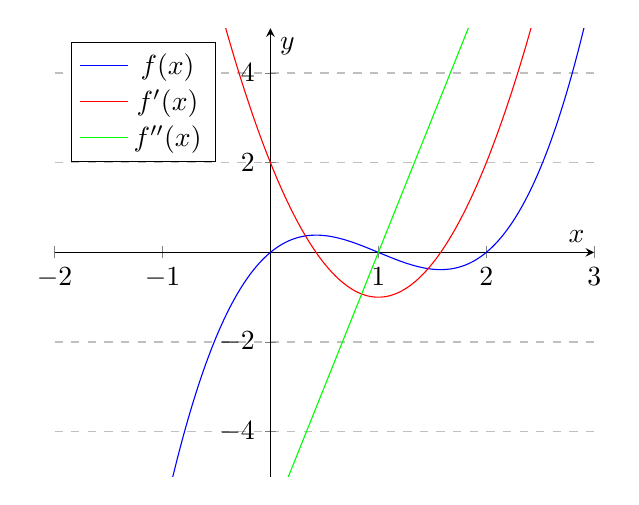
\begin{tikzpicture}
\begin{axis}[
    axis lines = middle,
    xlabel = \(x\),
    ylabel = {\(y\)},
    xmin=-2, xmax=3,
    ymin=-5, ymax=5,
    legend pos=north west,
    ymajorgrids=true,
    grid style=dashed,
]

% Original function f(x)
\addplot [
    domain=-1:3,
    samples=100,
    color=blue,
    smooth,
] {x^3 - 3*x^2 + 2*x};
\addlegendentry{\(f(x)\)}

% First derivative f'(x)
\addplot [
    domain=-1:3,
    samples=100,
    color=red,
    smooth,
] {3*x^2 - 6*x + 2};
\addlegendentry{\(f'(x)\)}

% Second derivative f''(x)
\addplot [
    domain=-1:3,
    samples=100,
    color=green,
    smooth,
] {6*x - 6};
\addlegendentry{\(f''(x)\)}

\end{axis}
\end{tikzpicture}
\end{center}

This graph illustrates the original function \( f(x) \) and its first and second derivatives, providing a visual representation of how each successive derivative relates to the original function.

\subsubsection*{Exercises on Higher-Order Derivatives}

\begin{exercise}
Find the first four derivatives of the function \( g(x) = \sin(x) \).
\end{exercise}

\begin{exercise}
If \( h(x) = e^{2x} \), compute \( h'''(x) \).
\end{exercise}

These exercises allow students to practice calculating higher-order derivatives, which is a crucial skill in advanced calculus and its applications.

\subsubsection*{Additional Exercises on Higher-Order Derivatives}

The following exercises aim to further reinforce the concept of higher-order derivatives through practical applications.

\begin{exercise}
Find the first three derivatives of the function \( p(t) = \ln(t^2 + 1) \).
\end{exercise}

\begin{exercise}
Given \( f(x) = \frac{1}{x^2 + 1} \), compute \( f''(x) \) and \( f'''(x) \).
\end{exercise}

\begin{exercise}
For the function \( g(x) = e^{-x} \cos(x) \), determine \( g'(x) \), \( g''(x) \), and \( g'''(x) \).
\end{exercise}

\begin{exercise}
Calculate the fourth derivative of \( h(x) = x^4 - 4x^3 + 6x^2 - 4x + 1 \).
\end{exercise}

\subsubsection*{Solutions to Additional Exercises on Higher-Order Derivatives}

\begin{solution}[to Exercise 1]
For \( p(t) = \ln(t^2 + 1) \), we find:
\[ p'(t) = \frac{2t}{t^2 + 1}, \quad p''(t) = \frac{2 - 2t^2}{(t^2 + 1)^2}, \quad p'''(t) = \frac{-8t(t^2 - 3)}{(t^2 + 1)^3}. \]
\end{solution}

\begin{solution}[to Exercise 2]
For \( f(x) = \frac{1}{x^2 + 1} \), we calculate:
\[ f''(x) = \frac{6x^2 - 2}{(x^2 + 1)^3}, \quad f'''(x) = \frac{-24x(x^2 - 1)}{(x^2 + 1)^4}. \]
\end{solution}

\begin{solution}[to Exercise 3]
For \( g(x) = e^{-x} \cos(x) \):
\[ g'(x) = -e^{-x} (\cos(x) + \sin(x)), \]
\[ g''(x) = e^{-x} (2\sin(x)), \]
\[ g'''(x) = e^{-x} (2\cos(x) - 2\sin(x)). \]
\end{solution}

\begin{solution}[to Exercise 4]
For \( h(x) = x^4 - 4x^3 + 6x^2 - 4x + 1 \):
\[ h''''(x) = 24. \]
\end{solution}

These exercises provide a comprehensive range of functions to practice differentiating, helping students to deepen their understanding of higher-order derivatives and their applications in various contexts.

\subsection{L'Hôpital's Rule for Indeterminate Forms}
\label{subsec:lhospitals_rule}

\begin{theorem}[L'Hôpital's Rule]
If the functions \( f(x) \) and \( g(x) \) are differentiable and \( \lim_{x \to c} f(x) = \lim_{x \to c} g(x) = 0 \) or \( \pm \infty \), and if \( \lim_{x \to c} \frac{f'(x)}{g'(x)} \) exists or equals \( \pm \infty \), then
\[ \lim_{x \to c} \frac{f(x)}{g(x)} = \lim_{x \to c} \frac{f'(x)}{g'(x)}. \]
\end{theorem}

\subsubsection*{Graphical Illustration}
To understand L'Hôpital's Rule, let's consider the indeterminate form \(\frac{0}{0}\). Suppose \( f(x) \) and \( g(x) \) approach 0 as \( x \) approaches \( c \), making \( \frac{f(x)}{g(x)} \) indeterminate at \( x = c \). 

% Graphical illustration using tikz
\begin{figure}[H]
\centering
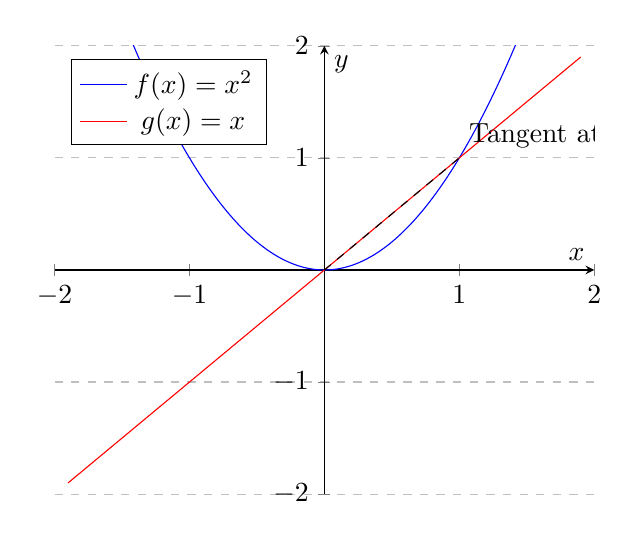
\begin{tikzpicture}
\begin{axis}[
    axis lines = middle,
    xlabel = \(x\),
    ylabel = {\(y\)},
    xmin=-2, xmax=2,
    ymin=-2, ymax=2,
    legend pos=north west,
    ymajorgrids=true,
    grid style=dashed,
]

% Plot f(x) and g(x)
\addplot[domain=-1.9:1.9, samples=200, blue] {x^2};
\addlegendentry{\(f(x) = x^2\)}

\addplot[domain=-1.9:1.9, samples=200, red] {x};
\addlegendentry{\(g(x) = x\)}

\draw[dashed] (axis cs:0,0) -- (axis cs:1,1);
\node[anchor=south west] at (axis cs:1,1) {Tangent at \(c\)};

\end{axis}
\end{tikzpicture}
\caption{Graphical interpretation of L'Hôpital's Rule}
\end{figure}

\subsubsection*{Applications}
L'Hôpital's Rule is particularly useful in calculus for resolving limits that result in indeterminate forms like \( \frac{0}{0} \) or \( \frac{\infty}{\infty} \). It simplifies complex limit evaluations, especially when direct substitution in the limit leads to an indeterminate form.

\subsubsection*{Examples}
\begin{example}
Evaluate \( \lim_{x \to 0} \frac{\sin(x)}{x} \).

\textbf{Solution:}
Direct substitution gives \(\frac{0}{0}\), an indeterminate form. Applying L'Hôpital's Rule:
\[ \lim_{x \to 0} \frac{\sin(x)}{x} = \lim_{x \to 0} \frac{\cos(x)}{1} = \cos(0) = 1. \]
\end{example}

\begin{example}
Find \( \lim_{x \to \infty} \frac{e^x}{x^2} \).

\textbf{Solution:}
Both numerator and denominator approach infinity as \( x \to \infty \). Applying L'Hôpital's Rule twice:
\[ \lim_{x \to \infty} \frac{e^x}{x^2} = \lim_{x \to \infty} \frac{e^x}{2x} = \lim_{x \to \infty} \frac{e^x}{2} = \infty. \]
\end{example}

\subsubsection*{Conclusion}
L'Hôpital's Rule streamlines the process of evaluating limits that lead to indeterminate forms, which are common in calculus. Its application requires understanding of derivatives and their properties.

\subsubsection*{Practice Problems}
To further strengthen your understanding of L'Hôpital's Rule, try solving the following problems:

\begin{problem}
Evaluate the limit: \( \lim_{x \to 0} \frac{e^x - 1}{x} \).
\end{problem}

\begin{problem}
Find the limit: \( \lim_{x \to \infty} \frac{\ln(x)}{x} \).
\end{problem}

\begin{problem}
Determine \( \lim_{x \to 0} \frac{\sin(2x)}{3x} \).
\end{problem}

\begin{problem}
Compute the limit: \( \lim_{x \to 0^+} x \ln(x) \).
\end{problem}

\begin{problem}
Evaluate \( \lim_{x \to 0} \frac{1 - \cos(x)}{x^2} \).
\end{problem}

\subsubsection*{Hints}
\begin{itemize}
  \item For problems that result in the \(\frac{0}{0}\) indeterminate form, apply L'Hôpital's Rule by differentiating the numerator and denominator separately.
  \item If the indeterminate form persists after the first application of the rule, you may need to apply L'Hôpital's Rule multiple times.
  \item Remember that understanding the behavior of functions as they approach a point is key to correctly applying L'Hôpital's Rule.
\end{itemize}

These problems are designed to cover various scenarios where L'Hôpital's Rule can be applied. They will help you develop a deeper understanding of how to deal with indeterminate forms in calculus.

\subsubsection*{Solutions to Practice Problems}

\begin{solution}[to Problem 1]
Evaluate \( \lim_{x \to 0} \frac{e^x - 1}{x} \).

\textit{Solution:}
Applying L'Hôpital's Rule, we differentiate the numerator and denominator:

\[
\lim_{x \to 0} \frac{e^x - 1}{x} = \lim_{x \to 0} \frac{e^x}{1} = e^0 = 1.
\]
\end{solution}

\begin{solution}[to Problem 2]
Find \( \lim_{x \to \infty} \frac{\ln(x)}{x} \).

\textit{Solution:}
Using L'Hôpital's Rule:

\[
\lim_{x \to \infty} \frac{\ln(x)}{x} = \lim_{x \to \infty} \frac{1/x}{1} = 0.
\]
\end{solution}

\begin{solution}[to Problem 3]
Determine \( \lim_{x \to 0} \frac{\sin(2x)}{3x} \).

\textit{Solution:}
Applying L'Hôpital's Rule:

\[
\lim_{x \to 0} \frac{\sin(2x)}{3x} = \lim_{x \to 0} \frac{2\cos(2x)}{3} = \frac{2}{3}.
\]
\end{solution}

\begin{solution}[to Problem 4]
Compute \( \lim_{x \to 0^+} x \ln(x) \).

\textit{Solution:}
This is an indeterminate form of type \( 0 \cdot (-\infty) \). Rewriting the expression:

\[
\lim_{x \to 0^+} x \ln(x) = \lim_{x \to 0^+} \frac{\ln(x)}{1/x}.
\]

Now applying L'Hôpital's Rule:

\[
\lim_{x \to 0^+} \frac{\ln(x)}{1/x} = \lim_{x \to 0^+} \frac{1/x}{-1/x^2} = \lim_{x \to 0^+} -x = 0.
\]
\end{solution}

\begin{solution}[to Problem 5]
Evaluate \( \lim_{x \to 0} \frac{1 - \cos(x)}{x^2} \).

\textit{Solution:}
Using L'Hôpital's Rule:

\[
\lim_{x \to 0} \frac{1 - \cos(x)}{x^2} = \lim_{x \to 0} \frac{\sin(x)}{2x} = \lim_{x \to 0} \frac{\cos(x)}{2} = \frac{1}{2}.
\]
\end{solution}

These solutions provide step-by-step application of L'Hôpital's Rule to solve the given limits. They illustrate the procedure of differentiating the numerator and denominator to resolve indeterminate forms.

\subsection{Implicit Differentiation}

\begin{method}
Implicit differentiation is used when a function is given in an implicit form \( F(x, y) = 0 \) rather than the explicit form \( y = f(x) \). It involves differentiating both sides of the equation with respect to \( x \) and solving for \( \frac{dy}{dx} \).
\end{method}

\subsection{Principle of Implicit Differentiation}
In implicit differentiation, each term involving \( y \) is differentiated using the chain rule, as \( y \) is a function of \( x \).

\example{Differentiate the equation \( x^2 + y^2 = 25 \) implicitly.}

\begin{solution}
Differentiating both sides with respect to \( x \):
\[ \frac{d}{dx}(x^2 + y^2) = \frac{d}{dx}(25), \]
\[ 2x + 2y \frac{dy}{dx} = 0. \]
Solving for \( \frac{dy}{dx} \):
\[ \frac{dy}{dx} = -\frac{x}{y}. \]
\end{solution}

\subsection{Graphical Representation of Implicit Functions}

\begin{center}
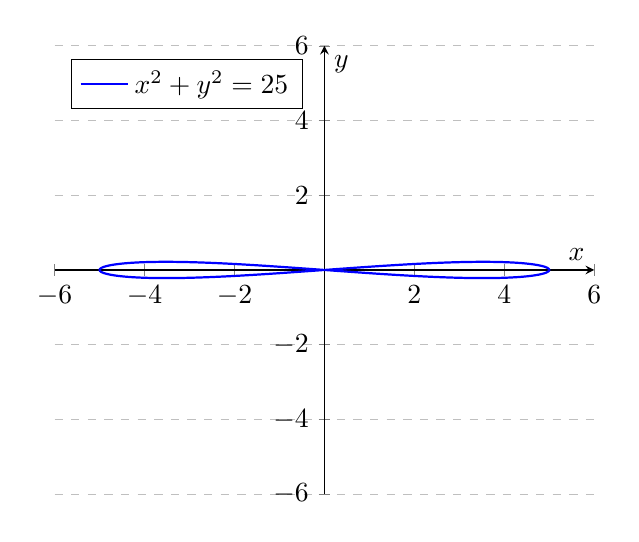
\begin{tikzpicture}
\begin{axis}[
    axis lines = middle,
    xlabel = \(x\),
    ylabel = \(y\),
    xmin=-6, xmax=6,
    ymin=-6, ymax=6,
    legend pos=north west,
    ymajorgrids=true,
    grid style=dashed,
]

% Implicit function x^2 + y^2 = 25
\addplot [
    data cs=polar,
    domain=0:360,
    samples=200,
    color=blue,
    thick,
] ({25^(0.5) * cos(x)}, {25^(0.5) * sin(x)});
\addlegendentry{\(x^2 + y^2 = 25\)}

\end{axis}
\end{tikzpicture}
\end{center}

This graph shows the circle defined by the equation \( x^2 + y^2 = 25 \). Implicit differentiation helps find the slope of the tangent at any point on this curve.

\subsection{Practical Engineering Example: Pressure and Volume in Thermodynamics}

\begin{example}
In thermodynamics, the relationship between the pressure \( P \), volume \( V \), and temperature \( T \) of a gas is often described by the equation \( PV = nRT \), where \( n \) is the number of moles of the gas and \( R \) is the universal gas constant. If the temperature is held constant, find the rate at which pressure changes with respect to volume.
\end{example}

\begin{solution}
Given the equation \( PV = nRT \) with constant \( T \), we differentiate implicitly with respect to \( V \):
\[ P\frac{dV}{dV} + V\frac{dP}{dV} = 0, \]
\[ P + V\frac{dP}{dV} = 0, \]
\[ \frac{dP}{dV} = -\frac{P}{V}. \]
This result indicates that the rate at which pressure changes with respect to volume is inversely proportional to the volume itself, assuming temperature remains constant. This principle is crucial in understanding how gases behave under compression or expansion in various engineering applications.
\end{solution}

\begin{discussion}
This example demonstrates the application of implicit differentiation in the field of thermodynamics, specifically in understanding how the properties of gases change under different conditions. Such principles are fundamental in engineering disciplines, especially in mechanical and chemical engineering.
\end{discussion}

\subsubsection*{Exercises on Implicit Differentiation}

\begin{exercise}
Use implicit differentiation to find \( \frac{dy}{dx} \) for the curve \( x^3 + y^3 - 3xy = 0 \).
\end{exercise}

\begin{exercise}
Find the slope of the tangent line to the ellipse \( 4x^2 + 9y^2 = 36 \) at the point \( (2, \sqrt{2}) \).
\end{exercise}

These exercises aim to provide hands-on experience with implicit differentiation, enhancing the understanding of this essential calculus technique.

\subsubsection*{More Exercises on Implicit Differentiation}

\begin{exercise}
Find \( \frac{dy}{dx} \) for the curve given by the equation \( \sin(xy) = x + y \).
\end{exercise}

\begin{exercise}
Differentiate implicitly to find the slope of the curve \( e^{x+y} = x^2 + y^2 \) at any point.
\end{exercise}

\begin{exercise}
For the curve defined by \( \ln(x) + \ln(y) = 1 \), find \( \frac{d^2y}{dx^2} \).
\end{exercise}

\begin{exercise}
Use implicit differentiation to find the slope of the tangent line to the curve \( x^4 + y^4 = 16 \) at the point \( (1, \sqrt[4]{15}) \).
\end{exercise}

\begin{exercise}
Find \( \frac{dy}{dx} \) for the ellipse \( 4x^2 + y^2 = 16 \) using implicit differentiation.
\end{exercise}

\subsubsection*{Solutions to More Exercises on Implicit Differentiation}

\begin{solution}[to Exercise 1]
Differentiating \( \sin(xy) = x + y \) implicitly:
\[ \cos(xy)(y + x\frac{dy}{dx}) = 1 + \frac{dy}{dx}, \]
\[ \frac{dy}{dx}(x\cos(xy) - 1) = 1 - y\cos(xy), \]
\[ \frac{dy}{dx} = \frac{1 - y\cos(xy)}{x\cos(xy) - 1}. \]
\end{solution}

\begin{solution}[to Exercise 2]
Differentiating \( e^{x+y} = x^2 + y^2 \):
\[ e^{x+y}(1 + \frac{dy}{dx}) = 2x + 2y\frac{dy}{dx}, \]
\[ \frac{dy}{dx}(e^{x+y} - 2y) = 2x - e^{x+y}, \]
\[ \frac{dy}{dx} = \frac{2x - e^{x+y}}{e^{x+y} - 2y}. \]
\end{solution}

\begin{solution}[to Exercise 3]
Differentiating \( \ln(x) + \ln(y) = 1 \):
\[ \frac{1}{x} + \frac{1}{y}\frac{dy}{dx} = 0, \]
\[ \frac{dy}{dx} = -\frac{y}{x}. \]
To find \( \frac{d^2y}{dx^2} \), differentiate \( \frac{dy}{dx} \) again:
\[ \frac{d^2y}{dx^2} = -\frac{x\frac{dy}{dx} - y}{x^2} = -\frac{-y^2/x - y}{x^2} = \frac{y(y + x)}{x^3}. \]
\end{solution}

\begin{solution}[to Exercise 4]
For \( x^4 + y^4 = 16 \) at \( (1, \sqrt[4]{15}) \):
\[ 4x^3 + 4y^3\frac{dy}{dx} = 0, \]
\[ \frac{dy}{dx} = -\frac{x^3}{y^3} = -\frac{1}{(\sqrt[4]{15})^3}. \]
\end{solution}

\begin{solution}[to Exercise 5]
For \( 4x^2 + y^2 = 16 \):
\[ 8x + 2y\frac{dy}{dx} = 0, \]
\[ \frac{dy}{dx} = -\frac{8x}{2y} = -\frac{4x}{y}. \]
\end{solution}

These exercises provide a diverse range of problems to practice implicit differentiation and help students understand its applications in different scenarios.

\section{Applications of Derivatives}
\subsection{Tangent Lines and Normal Lines}
\begin{application}
The equation of the tangent line to the curve \( y = f(x) \) at the point \( (a, f(a)) \) is given by \( y - f(a) = f'(a)(x - a) \). The normal line is perpendicular to the tangent line at the point of tangency.
\end{application}

\begin{example}
Consider the function \( f(x) = x^2 \). Find the equation of the tangent and normal lines to the curve at the point where \( x = 1 \).
\end{example}

\begin{solution}
First, we find the derivative of \( f(x) = x^2 \), which is \( f'(x) = 2x \). At \( x = 1 \), \( f'(1) = 2 \times 1 = 2 \). The equation of the tangent line at \( x = 1 \) is:
\[ y - 1 = 2(x - 1) \]
or
\[ y = 2x - 1. \]

To find the equation of the normal line, we use the fact that the slope of the normal line is the negative reciprocal of the tangent line's slope. Thus, the slope of the normal line is \( -\frac{1}{2} \), and its equation is:
\[ y - 1 = -\frac{1}{2}(x - 1) \]
or
\[ y = -\frac{1}{2}x + \frac{3}{2}. \]
\end{solution}

\begin{figure}[H]
\centering
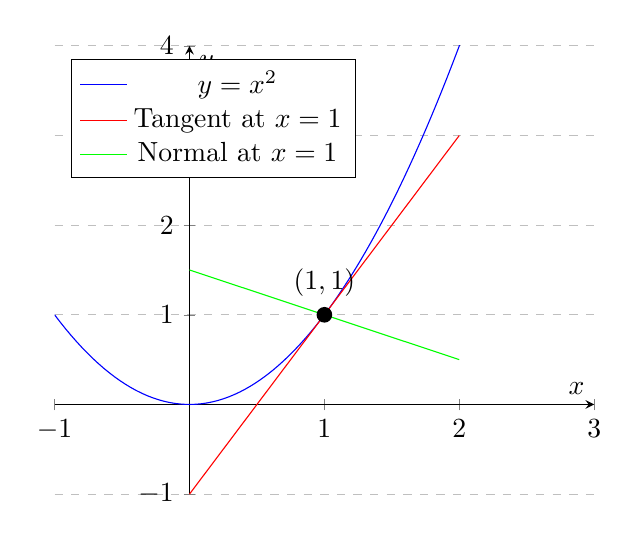
\begin{tikzpicture}
\begin{axis}[
    axis lines = center,
    xlabel = \(x\),
    ylabel = {\(y\)},
    xmin=-1, xmax=3,
    ymin=-1, ymax=4,
    legend pos=north west,
    ymajorgrids=true,
    grid style=dashed,
]

% Plotting the function f(x) = x^2
\addplot[domain=-1:3, samples=100, color=blue]{x^2};
\addlegendentry{\(y = x^2\)}

% Plotting the tangent line
\addplot[domain=0:2, samples=100, color=red]{2*x - 1};
\addlegendentry{Tangent at \(x=1\)}

% Plotting the normal line
\addplot[domain=0:2, samples=100, color=green]{-0.5*x + 1.5};
\addlegendentry{Normal at \(x=1\)}

% Point of tangency
\node[label={above:\((1,1)\)},circle,fill,inner sep=2pt] at (axis cs:1,1) {};

\end{axis}
\end{tikzpicture}
\caption{Graph of the function \(y = x^2\) with its tangent and normal lines at \(x = 1\).}
\end{figure}

\begin{discussion}
This example illustrates how to determine the equations of tangent and normal lines to a given curve at a specific point. The graphical representation helps in visualizing these concepts, which are fundamental in differential calculus and have various applications in fields such as engineering and physics.
\end{discussion}

\subsubsection*{Practice Problems on Tangent and Normal Lines}

\begin{problem}
Find the equations of the tangent and normal lines to the curve \( y = \sqrt{x} \) at the point where \( x = 4 \).
\end{problem}

\begin{problem}
Consider the function \( f(x) = \frac{1}{x} \). Determine the equation of the tangent line at the point \( x = 2 \) and the equation of the normal line at the same point.
\end{problem}

\begin{problem}
Given the function \( f(x) = 3x^3 - 2x + 1 \), compute the equations of the tangent and normal lines at the point where \( x = -1 \).
\end{problem}

\begin{problem}
For the function \( f(x) = \sin(x) \), find the equations of the tangent and normal lines at \( x = \frac{\pi}{4} \).
\end{problem}

\begin{problem}
Determine the equations of the tangent and normal lines to the curve given by \( y = \ln(x) \) at the point where \( x = e \) (where \( e \) is the base of the natural logarithm).
\end{problem}

\begin{problem}
Consider the curve defined by the equation \( x^2 + y^2 = 25 \). Find the equations of the tangent and normal lines at the point \( (3, 4) \) on the curve.
\end{problem}

\begin{discussion}
These problems involve different types of functions, including polynomial, trigonometric, logarithmic, and even a circle equation. Solving these problems will give students practice in applying the concepts of derivatives to find tangent and normal lines in various contexts.
\end{discussion}

\subsubsection*{Solutions to Practice Problems on Tangent and Normal Lines}

\begin{solution}[to Problem 1]
The function is \( y = \sqrt{x} \). Its derivative is \( \frac{1}{2\sqrt{x}} \). At \( x = 4 \), the slope of the tangent line is \( \frac{1}{2\sqrt{4}} = \frac{1}{4} \). The equation of the tangent line is given by \( y - f(a) = f'(a)(x - a) \), which simplifies to \( y - 2 = \frac{1}{4}(x - 4) \). The normal line is perpendicular to the tangent line, so its slope is the negative reciprocal, \( -4 \). The equation of the normal line is \( y - 2 = -4(x - 4) \).
\end{solution}

\begin{solution}[to Problem 2]
For \( f(x) = \frac{1}{x} \), \( f'(x) = -\frac{1}{x^2} \). At \( x = 2 \), \( f'(2) = -\frac{1}{4} \), so the tangent line is \( y - \frac{1}{2} = -\frac{1}{4}(x - 2) \). The slope of the normal line is \( 4 \), so its equation is \( y - \frac{1}{2} = 4(x - 2) \).
\end{solution}

\begin{solution}[to Problem 3]
The derivative of \( f(x) = 3x^3 - 2x + 1 \) is \( f'(x) = 9x^2 - 2 \). At \( x = -1 \), \( f'(-1) = 7 \). The equation of the tangent line is \( y - 2 = 7(x + 1) \). The normal line has a slope of \( -\frac{1}{7} \), so its equation is \( y - 2 = -\frac{1}{7}(x + 1) \).
\end{solution}

\begin{solution}[to Problem 4]
For \( f(x) = \sin(x) \), \( f'(x) = \cos(x) \). At \( x = \frac{\pi}{4} \), \( f'\left(\frac{\pi}{4}\right) = \frac{\sqrt{2}}{2} \). The tangent line equation is \( y - \frac{\sqrt{2}}{2} = \frac{\sqrt{2}}{2}\left(x - \frac{\pi}{4}\right) \). The normal line has a slope of \( -\frac{\sqrt{2}}{2} \), with its equation being \( y - \frac{\sqrt{2}}{2} = -\frac{\sqrt{2}}{2}\left(x - \frac{\pi}{4}\right) \).
\end{solution}

\begin{solution}[to Problem 5]
For \( y = \ln(x) \), \( \frac{dy}{dx} = \frac{1}{x} \). At \( x = e \), the derivative is \( \frac{1}{e} \). The tangent line equation is \( y - 1 = \frac{1}{e}(x - e) \). The normal line's slope is \( -e \), so its equation is \( y - 1 = -e(x - e) \).
\end{solution}

\begin{solution}[to Problem 6]
For the circle \( x^2 + y^2 = 25 \), implicit differentiation gives \( 2x + 2yy' = 0 \). At \( (3, 4) \), \( y' = -\frac{3}{4} \). The equation of the tangent line is \( y - 4 = -\frac{3}{4}(x - 3) \). The normal line, with a slope of \( \frac{4}{3} \), has the equation \( y - 4 = \frac{4}{3}(x - 3) \).
\end{solution}

\begin{discussion}
These solutions demonstrate the application of derivatives to find equations of tangent and normal lines. They involve direct computation of derivatives, using implicit differentiation, and understanding the relationship between slopes of tangent and normal lines.
\end{discussion}

\subsection{Increasing and Decreasing Functions}
\begin{theorem}
A function \( f \) is increasing on an interval if, for any two numbers \( x_1 \) and \( x_2 \) in the interval with \( x_1 < x_2 \), we have \( f(x_1) \leq f(x_2) \). Similarly, \( f \) is decreasing on an interval if \( f(x_1) \geq f(x_2) \) for \( x_1 < x_2 \) in the interval. This can often be determined by analyzing the sign of its derivative \( f' \).
\end{theorem}

\begin{example}
Consider the function \( f(x) = x^3 - 3x^2 + 2 \). To determine where the function is increasing or decreasing, we first find its derivative: \( f'(x) = 3x^2 - 6x \). Setting \( f'(x) = 0 \), we find critical points at \( x = 0 \) and \( x = 2 \).

We then test intervals around these critical points to determine the sign of \( f'(x) \):
\begin{itemize}
    \item For \( x < 0 \), take \( x = -1 \): \( f'(-1) = -3 - 6 = -9 \) (negative, so \( f \) is decreasing).
    \item For \( 0 < x < 2 \), take \( x = 1 \): \( f'(1) = 3 - 6 = -3 \) (negative, so \( f \) is still decreasing).
    \item For \( x > 2 \), take \( x = 3 \): \( f'(3) = 27 - 18 = 9 \) (positive, so \( f \) is increasing).
\end{itemize}

Thus, \( f(x) \) is decreasing on \((- \infty, 2]\) and increasing on \([2, +\infty)\).
\end{example}

% Graph of the function
\begin{center}
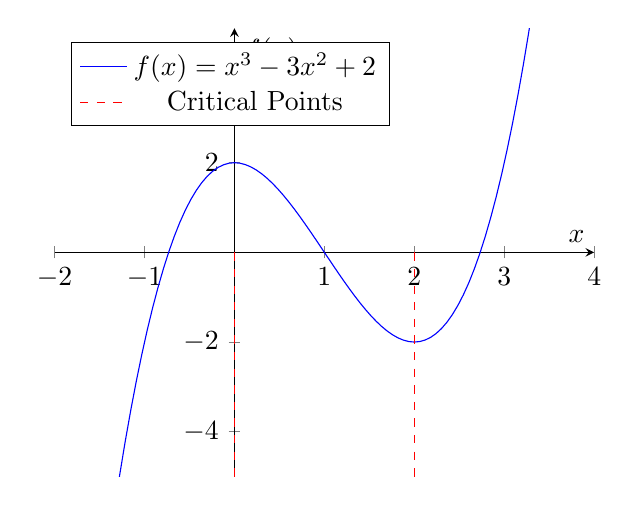
\begin{tikzpicture}
\begin{axis}[
    axis lines = middle,
    xlabel = \(x\),
    ylabel = {\(f(x)\)},
    ymin = -5, ymax = 5,
    xmin = -2, xmax = 4,
    legend pos=north west
]
\addplot [
    domain=-2:4, 
    samples=100, 
    color=blue,
    ]
    {x^3 - 3*x^2 + 2};
\addlegendentry{\(f(x) = x^3 - 3x^2 + 2\)}

% Adding dashed lines for critical points
\draw [dashed, red] (axis cs:0,0) -- (axis cs:0,-5);
\draw [dashed, red] (axis cs:2,0) -- (axis cs:2,-5);
\addlegendimage{dashed, red}
\addlegendentry{Critical Points}

\end{axis}
\end{tikzpicture}
\end{center}

\begin{discussion}
This example illustrates how to find intervals where a function is increasing or decreasing. By examining the derivative, we can identify critical points and the behavior of the function around these points. The graph visually confirms these findings.
\end{discussion}

\subsubsection*{Practice Problems on Increasing and Decreasing Functions}
\begin{problem}
Determine the intervals where the function \( f(x) = x^2 - 4x + 3 \) is increasing and decreasing.
\end{problem}

\begin{problem}
Given the function \( g(x) = \frac{1}{x} \), find the intervals where the function is increasing and where it is decreasing.
\end{problem}

\begin{problem}
For the function \( h(x) = e^{-x} \), identify the intervals of increase and decrease.
\end{problem}

\begin{problem}
Consider the function \( p(x) = x^3 - 9x^2 + 24x - 15 \). Analyze the function's increasing and decreasing behavior.
\end{problem}

\begin{problem}
Let \( q(x) = \sin(x) \) on the interval \( [0, 2\pi] \). Determine where the function is increasing and decreasing.
\end{problem}

\begin{discussion}
These problems involve different types of functions, including polynomial, rational, exponential, and trigonometric functions. Students should first find the derivative of the function, determine critical points, and then analyze the sign of the derivative on intervals around these points to conclude where the function is increasing or decreasing.
\end{discussion}

\subsubsection*{Solutions to Practice Problems}

\begin{solution}[Problem 1]
To find where \( f(x) = x^2 - 4x + 3 \) is increasing and decreasing, we first find its derivative:
\[ f'(x) = 2x - 4. \]
Setting \( f'(x) = 0 \), we find the critical point at \( x = 2 \). 

Examining the sign of \( f'(x) \) around this point:
\begin{itemize}
    \item For \( x < 2 \), say \( x = 1 \), \( f'(1) = -2 \), so \( f(x) \) is decreasing.
    \item For \( x > 2 \), say \( x = 3 \), \( f'(3) = 2 \), so \( f(x) \) is increasing.
\end{itemize}
Thus, \( f(x) \) is decreasing on \((- \infty, 2)\) and increasing on \((2, \infty)\).
\end{solution}

\begin{solution}[Problem 2]
For \( g(x) = \frac{1}{x} \), the derivative is
\[ g'(x) = -\frac{1}{x^2}. \]
Since \( g'(x) \) is always negative for \( x \neq 0 \), \( g(x) \) is always decreasing on its domain.
\end{solution}

\begin{solution}[Problem 3]
For \( h(x) = e^{-x} \), the derivative is
\[ h'(x) = -e^{-x}. \]
Since \( h'(x) < 0 \) for all \( x \), \( h(x) \) is always decreasing.
\end{solution}

\begin{solution}[Problem 4]
Consider \( p(x) = x^3 - 9x^2 + 24x - 15 \). The derivative is
\[ p'(x) = 3x^2 - 18x + 24. \]
Setting \( p'(x) = 0 \) yields \( x = 2 \) and \( x = 4 \) as critical points.

Checking intervals around these points:
\begin{itemize}
    \item For \( x < 2 \), \( p'(x) > 0 \), so \( p(x) \) is increasing.
    \item For \( 2 < x < 4 \), \( p'(x) < 0 \), so \( p(x) \) is decreasing.
    \item For \( x > 4 \), \( p'(x) > 0 \), so \( p(x) \) is increasing.
\end{itemize}
Therefore, \( p(x) \) is increasing on \((- \infty, 2) \cup (4, \infty)\) and decreasing on \((2, 4)\).
\end{solution}

\begin{solution}[Problem 5]
For \( q(x) = \sin(x) \) on \( [0, 2\pi] \), the derivative is
\[ q'(x) = \cos(x). \]
We find critical points where \( \cos(x) = 0 \), which are \( x = \frac{\pi}{2} \) and \( x = \frac{3\pi}{2} \).

Examining the sign of \( q'(x) \):
\begin{itemize}
    \item For \( 0 < x < \frac{\pi}{2} \), \( q'(x) > 0 \), so \( q(x) \) is increasing.
    \item For \( \frac{\pi}{2} < x < \frac{3\pi}{2} \), \( q'(x) < 0 \), so \( q(x) \) is decreasing.
    \item For \( \frac{3\pi}{2} < x < 2\pi \), \( q'(x) > 0 \), so \( q(x) \) is increasing.
\end{itemize}
Thus, \( q(x) \) is increasing on \((0, \frac{\pi}{2}) \cup (\frac{3\pi}{2}, 2\pi)\) and decreasing on \((\frac{\pi}{2}, \frac{3\pi}{2})\).
\end{solution}

% HERE

\subsection{Maxima and Minima}
\begin{method}
Critical points, where \( f'(x) = 0 \) or \( f'(x) \) does not exist, are potential locations of local maxima or minima.
\end{method}

\subsection{Concavity and Inflection Points}
\begin{discussion}
A function is concave up (down) where its second derivative \( f'' \) is positive (negative). Points where \( f'' \) changes sign are inflection points.
\end{discussion}

\subsection{Optimization Problems}
\begin{application}
Optimization involves finding the maximum or minimum values of a function subject to certain constraints, often using derivatives.
\end{application}

\subsection{Related Rates}
\begin{method}
Related rates problems involve finding the rate at which one quantity changes with respect to another using the chain rule.
\end{method}


\section{Rolle's, Mean Value, and Extreme Value Theorems}
\subsection{Rolle's Theorem}
\begin{theorem}[Rolle's Theorem]
If a function \( f \) is continuous on the closed interval \([a, b]\), differentiable on the open interval \((a, b)\), and \(f(a) = f(b)\), then there exists at least one \(c\) in the interval \((a, b)\) such that \(f'(c) = 0\).
\end{theorem}

\begin{center}
\begin{tikzpicture}
    \begin{axis}[
        axis lines = middle,
        xlabel = \(x\),
        ylabel = \(f(x)\),
        xmin = 0, xmax = 3,
        ymin = -1, ymax = 2,
        legend style={at={(0.95,0.95)}, anchor=north east}
    ]
    % Rolle's theorem example function
    \addplot [
        domain=0:3,
        samples=100,
        color=blue,
    ] 
    {(x-1)*(x-3)};
    \addlegendentry{\(f(x) = (x-1)(x-3)\)}
    
    % Tangent line (horizontal) at critical point
    \draw[dashed, color=red] (axis cs:1,0) -- (axis cs:3,0);

    % Critical points
    \addplot[holdot] coordinates {(1,0) (3,0)};
    \end{axis}
\end{tikzpicture}
\end{center}

\subsection{Mean Value Theorem}
\begin{theorem}[Mean Value Theorem]
If a function \( f \) is continuous on \([a, b]\) and differentiable on \((a, b)\), then there exists at least one \(c\) in \((a, b)\) such that \(f'(c) = \frac{f(b) - f(a)}{b - a}\).
\end{theorem}

\begin{center}
\begin{tikzpicture}
    \begin{axis}[
        axis lines = middle,
        xlabel = \(x\),
        ylabel = \(f(x)\),
        xmin = 0, xmax = 3,
        ymin = 0, ymax = 2,
        legend style={at={(0.95,0.95)}, anchor=north east}
    ]
    % Mean value theorem example function
    \addplot [
        domain=0:3,
        samples=100,
        color=blue,
    ] 
    {x^2};
    \addlegendentry{\(f(x) = x^2\)}

    % Secant line
    \addplot [
        domain=1:2,
        samples=2,
        color=green,
    ] 
    {x + 1};
    \addlegendentry{Secant line}

    % Tangent line at c
    \addplot [
        domain=1:2,
        samples=2,
        color=red,
    ] 
    {2*x};
    \addlegendentry{Tangent line at \(c\)}

    % Points a and b
    \addplot[holdot] coordinates {(1,1) (2,4)};

    \end{axis}
\end{tikzpicture}
\end{center}

\subsection{Extreme Value Theorem}
\begin{theorem}[Extreme Value Theorem]
If a function \( f \) is continuous on a closed interval \([a, b]\), then \( f \) must attain a maximum and a minimum, each at least once on that interval.
\end{theorem}

\begin{center}
\begin{tikzpicture}
    \begin{axis}[
        axis lines = middle,
        xlabel = \(x\),
        ylabel = \(f(x)\),
        xmin = 0, xmax = 3,
        ymin = -1, ymax = 2,
        legend style={at={(0.95,0.95)}, anchor=north east}
    ]
    % Extreme value theorem example function
    \addplot [
        domain=0:3,
        samples=100,
        color=blue,
    ] 
    {sin(deg(x)) + 1};
    \addlegendentry{\(f(x) = \sin(x) + 1\)}

    % Maximum and minimum points
    \addplot[soldot] coordinates {(1.57,2) (4.71,0)};
    \end{axis}
\end{tikzpicture}
\end{center}

These theorems are fundamental in calculus and provide critical insights into the behavior of differentiable functions. Rolle's Theorem and the Mean Value Theorem connect the properties of derivatives to the shape of a function's graph, while the Extreme Value Theorem guarantees the existence of global maximum and minimum values under certain conditions.

\subsubsection*{Exercises on Rolle's, Mean Value, and Extreme Value Theorems}

The following exercises will help you apply and understand the concepts of Rolle's Theorem, Mean Value Theorem, and Extreme Value Theorem.

\begin{exercise}
Given the function \( f(x) = x^3 - 6x^2 + 9x \) on the interval \([0, 3]\), verify if Rolle's Theorem can be applied. If so, find the value of \( c \) in the interval where \( f'(c) = 0 \).
\end{exercise}

\begin{exercise}
Use the Mean Value Theorem to find a value \( c \) in the interval \([1, 4]\) such that the tangent line at \( c \) is parallel to the secant line joining the points \((1, f(1))\) and \((4, f(4))\) for the function \( f(x) = x^2 \).
\end{exercise}

\begin{exercise}
Consider the function \( g(x) = \sin(x) \) on the interval \([0, \pi]\). Use the Extreme Value Theorem to discuss the existence of global maximum and minimum values of \( g(x) \) on this interval.
\end{exercise}

\begin{exercise}
For the function \( h(x) = \frac{1}{x} \) on the interval \([1, 3]\), determine if the Mean Value Theorem applies. If it does, find the value of \( c \) that satisfies the theorem.
\end{exercise}

\subsubsection*{Solutions to Exercises on Rolle's, Mean Value, and Extreme Value Theorems}

\begin{solution}[to Exercise 1]
First, we check if \( f(a) = f(b) \) for \( a = 0 \) and \( b = 3 \):
\[ f(0) = 0^3 - 6 \times 0^2 + 9 \times 0 = 0, \]
\[ f(3) = 3^3 - 6 \times 3^2 + 9 \times 3 = 0. \]
Since \( f(0) = f(3) \) and \( f(x) \) is continuous and differentiable on \([0, 3]\), Rolle's Theorem applies. 

To find \( c \), we solve \( f'(x) = 0 \):
\[ f'(x) = 3x^2 - 12x + 9, \]
\[ 0 = 3x^2 - 12x + 9. \]
Solving this quadratic equation gives the value of \( c \) in the interval \([0, 3]\).
\end{solution}

\begin{solution}[to Exercise 2]
For \( f(x) = x^2 \), the Mean Value Theorem states there exists a \( c \) in \([1, 4]\) such that:
\[ f'(c) = \frac{f(4) - f(1)}{4 - 1}. \]
Since \( f'(x) = 2x \), we find \( c \) by solving:
\[ 2c = \frac{4^2 - 1^2}{4 - 1}. \]
\end{solution}

\begin{solution}[to Exercise 3]
The function \( g(x) = \sin(x) \) is continuous on \([0, \pi]\). By the Extreme Value Theorem, it attains a maximum and minimum on this interval. The maximum is at \( x = \frac{\pi}{2} \) and the minimum at \( x = 0 \) or \( x = \pi \).
\end{solution}

\begin{solution}[to Exercise 4]
Since \( h(x) = \frac{1}{x} \) is continuous and differentiable on \([1, 3]\), the Mean Value Theorem applies. To find \( c \), solve:
\[ h'(c) = \frac{h(3) - h(1)}{3 - 1}, \]
where \( h'(x) = -\frac{1}{x^2} \). Solving this will give the value of \( c \).
\end{solution}

These exercises and solutions provide practical applications of Rolle's Theorem, Mean Value Theorem, and Extreme Value Theorem, reinforcing their concepts through specific examples.





\chapter{Integration}
\section{Antiderivatives}
\subsection{Definition and Basic Techniques}
\begin{definition}
An antiderivative of a function \( f(x) \) is a function \( F(x) \) such that \( F'(x) = f(x) \).
\end{definition}
\begin{example}
An antiderivative of \( f(x) = 2x \) is \( F(x) = x^2 + C \), where \( C \) is a constant.
\end{example}

\subsection{Indefinite Integrals}
\begin{definition}
The indefinite integral of \( f(x) \), denoted \( \int f(x) \, dx \), represents the collection of all its antiderivatives.
\end{definition}

\subsection{Initial Value Problems}
\begin{problem}
Given a differential equation \( f'(x) = g(x) \) and an initial condition \( f(x_0) = y_0 \), find the function \( f(x) \).
\end{problem}

\section{Definite Integrals}
\subsection{Definition and Interpretation}
\begin{definition}
The definite integral of \( f(x) \) from \( a \) to \( b \), denoted \( \int_a^b f(x) \, dx \), is the limit of the sum of areas of rectangles under the curve of \( f(x) \) as the width of the rectangles approaches zero.
\end{definition}

\subsection{Properties of Definite Integrals}
\begin{theorem}
Properties include linearity, additivity, and the fact that the integral from \( a \) to \( a \) is zero.
\end{theorem}

\subsection{Fundamental Theorem of Calculus}
\begin{theorem}
If \( F \) is an antiderivative of \( f \) on an interval, then \( \int_a^b f(x) \, dx = F(b) - F(a) \).
\end{theorem}

\subsection{Numerical Integration Methods}
\begin{method}
Methods include the Trapezoidal Rule and Simpson's Rule, which provide approximations of definite integrals.
\end{method}

\section{Applications of Integrals}
\subsection{Area Between Curves}
\begin{application}
The area between curves \( f(x) \) and \( g(x) \) from \( a \) to \( b \) is \( \int_a^b |f(x) - g(x)| \, dx \).
\end{application}

\subsection{Volumes of Solids of Revolution}
\begin{application}
The volume of a solid obtained by rotating a region about an axis can be found using the Disk or Washer methods.
\end{application}

\subsection{Arc Length and Surface Area}
\begin{method}
Formulas for the arc length of a curve and the surface area of a solid of revolution involve definite integrals.
\end{method}

\subsection{Work and Fluid Forces}
\begin{application}
Work done in moving an object and the force exerted by a fluid can be calculated using integration.
\end{application}

\chapter{Advanced Topics in Calculus}
\section{Sequences and Series}
\subsection{Convergence and Divergence}
\begin{definition}
A sequence \( \{a_n\} \) converges if it approaches a limit as \( n \) goes to infinity. A series \( \sum a_n \) converges if the sequence of its partial sums converges.
\end{definition}

\subsection{Tests for Convergence}
\begin{method}
Tests include the Integral Test, Comparison Test, Ratio Test, and Root Test.
\end{method}

\subsection{Power Series and Taylor Series}
\begin{definition}
A power series is a series of the form \( \sum_{n=0}^\infty a_n (x - c)^n \). A Taylor series is a power series that represents a function.
\end{definition}

\section{Multivariable Calculus}
\subsection{Functions of Several Variables}
\begin{definition}
A function of several variables is a function that takes several inputs and produces a single output.
\end{definition}

\subsection{Partial Derivatives}
\begin{definition}
The partial derivative of a function with respect to one of its variables is its derivative with respect to that variable, holding the other variables constant.
\end{definition}

\subsection{Multiple Integrals}
\begin{definition}
Multiple integrals involve integration over more than one variable, such as double and triple integrals.
\end{definition}

\subsection{Vector Calculus}
\begin{discussion}
Vector calculus involves differentiation and integration of vector fields, including topics like gradient, divergence, and curl.
\end{discussion}

\section{Differential Equations}
\subsection{First Order Differential Equations}
\begin{method}
Methods for solving include separation of variables, integrating factors, and exact equations.
\end{method}

\subsection{Second Order Linear Differential Equations}
\begin{method}
Includes homogeneous and non-homogeneous equations, characteristic equations, and particular solutions.
\end{method}

\subsection{Systems of Differential Equations}
\begin{discussion}
Systems of differential equations involve several interrelated differential equations and can be solved using matrix methods and eigenvalues.
\end{discussion}

\section{Conclusion}
\paragraph{}
This concludes the math currently included in CiB. Please fork the LaTeX source code for CiB (available on GitHub) and create your own book that chooses the facts and exercises most relevant to you! Also, starring the CiB project on GitHub would be greatly appreciated! Thanks for reading CiB!


% --- Appendices ---
\clearpage
\addcontentsline{toc}{chapter}{Appendices}
\appendix
\renewcommand{\thechapter}{\Roman{chapter}} % Ensuring chapters are numbered as I, II, III, etc.

%\appendix
\chapter{Basic GitHub Guide}
\section*{A Quick Start to Your GitHub Journey}

Welcome to the fascinating world of GitHub, a platform that has revolutionized the way we collaborate on projects, share code, and build software together. Whether you are a programmer, a writer, or a mathematician, GitHub provides a set of powerful tools to help you collaborate with others, manage your projects, and contribute to the vast world of open-source software. In this guide, we will walk you through the foundational steps to get started with GitHub, helping you to navigate, contribute, and make the most out of this incredible platform.

\subsection*{Creating Your GitHub Account}

The first step to joining the GitHub community is to create an account. Here’s how you can do it:

\begin{enumerate}
    \item Visit the \href{https://github.com/}{GitHub website}.
    \item Click on the “Sign up” button.
    \item Fill in the required information, including your username, email address, and password.
    \item Verify your account and complete the sign-up process.
\end{enumerate}

Once you have created your account, take a moment to explore your new GitHub dashboard. Here, you will find a variety of tools and features that will help you manage your projects, collaborate with others, and discover new and interesting repositories.

\subsection*{Creating Your First Repository}

A repository (or “repo”) is a digital directory where you can store your project files. Here’s how you can create your first repository:

\begin{enumerate}
    \item From your GitHub dashboard, click on the “New” button to create a new repository.
    \item Give your repository a name and provide a brief description.
    \item Initialize this repository with a README file. (This is an optional step, but it’s a good practice to include a README file in every repository to explain what your project is about.)
    \item Click “Create repository.”
\end{enumerate}

Congratulations! You have just created your first GitHub repository. You can now start adding files, collaborating with others, and managing your project right from GitHub.

\subsection*{Making Changes and Commits}

GitHub uses Git, a version control system, to keep track of changes made to your project. Here’s a quick guide on how to make changes and commits:

\begin{enumerate}
    \item Navigate to your repository on GitHub.
    \item Find the file you want to edit, and click on it.
    \item Click the pencil icon to start editing.
    \item Make your changes and then scroll down to the “Commit changes” section.
    \item Provide a commit message that explains the changes you made.
    \item Choose whether you want to commit directly to the main branch or create a new branch for your changes.
    \item Click “Commit changes.”
\end{enumerate}

Your changes are now saved, and a new commit is created. Every commit has a unique ID, making it easy to track changes, revert to previous versions, and collaborate with others.

\subsection*{Collaborating with Others}

One of the biggest strengths of GitHub is its collaborative nature. Here are some ways you can collaborate with others:

\begin{itemize}
    \item \textbf{Forking:} You can fork a repository, create your own copy, make changes, and then propose those changes back to the original project.
    \item \textbf{Issues:} Use issues to report bugs, request new features, or start a discussion with the community.
    \item \textbf{Pull Requests:} Propose changes to a project by creating a pull request. This allows others to review your changes, discuss them, and eventually merge them into the project.
\end{itemize}

\subsection*{Conclusion: Embarking on Your GitHub Adventure}

Now that you have a basic understanding of GitHub and how it works, you are ready to embark on your GitHub adventure. Explore repositories, contribute to open-source projects, collaborate with others, and build amazing things together. Remember, the GitHub community is vast and supportive, and there is a wealth of knowledge and resources available to help you along the way. Happy coding!


\chapter{Basic Python and Colab Guide}
\section*{Introduction to Python for Calculus}

Python's versatility in mathematics, science, engineering, and data analysis stems from its simplicity and extensive library ecosystem. This guide will delve into Python packages essential for math and calculus, showcasing their utility in Google Colab notebooks.

\subsection*{Setting Up Python and Google Colab}

Google Colab is a free, cloud-based platform enabling Python programming in a browser. It offers free computational resources, ideal for Python learning and experimentation.

Visit \href{https://colab.research.google.com/}{Google Colab} to start. Create a new notebook, and use code cells to write and execute Python code with Shift+Enter.

\subsection*{Important Python Packages for Calculus}

\subsubsection*{NumPy}
NumPy, fundamental for scientific computing, offers support for large, multi-dimensional arrays and matrices, along with various mathematical functions.

\subsubsection*{SymPy}
SymPy, a library for symbolic mathematics, allows algebraic manipulations and equation solving symbolically, perfect for calculus operations like differentiation and integration.

\subsubsection*{Matplotlib}
Matplotlib, a Python plotting library, creates static, interactive, and animated visualizations, useful for graphing functions and data in calculus.

\subsubsection*{Pandas}
Pandas provide high-performance, easy-to-use data structures, and data analysis tools, invaluable for handling and analyzing mathematical data.

\subsubsection*{SciPy}
SciPy extends NumPy by adding a collection of algorithms and high-level commands for data manipulation and visualization.

\subsection*{Examples and Applications}

\subsubsection*{Calculating Derivatives and Integrals with SymPy}
Illustrate using SymPy to compute derivatives and integrals of functions.

\subsubsection*{Data Visualization with Matplotlib and Pandas}
Demonstrate graphing functions and datasets, highlighting calculus concepts.

\subsubsection*{Solving Equations with SciPy}
Show how to solve equations that commonly appear in calculus.

\subsubsection*{Numerical Methods in Python}
Discuss Python's capabilities in numerical differentiation and integration, useful in calculus.

\subsubsection*{Using Python for Limits and Continuity}
Examples showcasing how Python can help in understanding limits and continuity in functions.

\subsection*{Interactive Learning with Google Colab}
Highlight the benefits of using Colab notebooks for interactive calculus learning, including real-time collaboration and easy sharing.


\subsection*{Creating a Colab Notebook for Practice Problems}

In this section, we will guide you through creating a Google Colab notebook to solve calculus practice problems using Python.

\subsubsection*{Setting Up Your Colab Notebook}
To start solving calculus problems with Python:

\begin{enumerate}
    \item Open \href{https://colab.research.google.com/}{Google Colab}.
    \item Choose 'New Notebook' to create a blank notebook.
    \item Rename the notebook to something descriptive, like 'Calculus Practice'.
\end{enumerate}

\subsubsection*{Installing Necessary Libraries}
At the beginning of your notebook, install any necessary Python libraries. For these exercises, ensure NumPy, SymPy, and Matplotlib are available:

\begin{verbatim}
Remove # if the following packages are not installed:
# !pip install numpy sympy matplotlib
\end{verbatim}

\subsubsection*{Solving Exercise 1: Graphing a Linear Function}
Let's solve the first exercise, which involves graphing a linear function.

\begin{verbatim}
import numpy as np
import matplotlib.pyplot as plt

# Define the function
def f(x):
    return 3*x - 2

# Generate x values
x = np.linspace(-10, 10, 400)

# Plot the function
plt.plot(x, f(x))
plt.xlabel('x')
plt.ylabel('f(x)')
plt.title('Graph of f(x) = 3x - 2')
plt.grid(True)
plt.show()

# Slope and y-intercept
print("Slope: 3")
print("Y-intercept: -2")
\end{verbatim}

\subsubsection*{Solving Exercise 2: Identifying Undefined Points in a Function}
Now, let's address the second exercise, which requires identifying for what values the function \( g(x) = \frac{1}{x} \) is undefined.

\begin{verbatim}
import sympy as sp

x = sp.symbols('x')
g = 1/x

# Display the function
sp.plot(g, (x, -10, 10), title='Graph of g(x) = 1/x',
        xlabel='x', ylabel='g(x)', ylim=(-10, 10))

# Identifying undefined points
print("g(x) is undefined for x = 0")
\end{verbatim}

\subsection*{Accessing the Completed Colab Notebook}

The Colab notebook we've discussed is available for viewing and interaction. You can access it by clicking on the following link: \href{https://colab.research.google.com/drive/1HF-cmwqfIZ803i1i-CFyR7ssWsDt7WvV}{Finished Colab Notebook on Graphing and Analysis}. This link will take you directly to the notebook hosted on Google Colab, where you can view the complete code and run it yourself.

\url{https://colab.research.google.com/drive/1HF-cmwqfIZ803i1i-CFyR7ssWsDt7WvV}

\subsection*{Adding the Notebook to Your GitHub Repository}

If you have downloaded the Colab notebook to your local machine and want to add it to your Git repository, follow these terminal commands on your Ubuntu machine:

\begin{verbatim}
# Navigate to your local Git repository directory
cd path/to/your/repo

# Add the Colab notebook file to the repository
git add name_of_the_notebook.ipynb

# Commit the addition with a descriptive message
git commit -m "Add Colab notebook for calculus exercises"

# Push the changes to the remote GitHub repository
git push origin main
\end{verbatim}

%Replace `path/to/your/repo` with the actual path to your local Git repository and `name_of_the_notebook.ipynb` with the filename of your Colab notebook.

\subsubsection*{Using Colab Notebooks for Problem Solving}
These examples demonstrate how you can use Google Colab and Python to solve and visualize calculus problems. You can use similar steps to tackle other exercises, explore different functions, and deepen your understanding of calculus concepts.

\subsection*{Conclusion: Interactive Learning with Colab Notebooks}

Google Colab notebooks offer an interactive and accessible way to explore calculus using Python. By integrating theoretical concepts with computational examples, students can gain a deeper understanding of calculus. We encourage you to use these notebooks to solve exercises, visualize mathematical concepts, and explore the vast possibilities that Python and Colab offer.


\subsection*{Conclusion: Python and Colab in Calculus}

Python, with its comprehensive libraries, offers a powerful toolset for calculus exploration. Combined with Google Colab, it provides an accessible, interactive platform for learning and experimentation. Embrace Python and Colab to enhance your understanding of calculus and to explore mathematical problems creatively and efficiently.


\chapter{Basic \LaTeX\ Guide}
\section*{A Quick Start to Your \LaTeX\ Journey}

Welcome to the immersive world of \LaTeX, a typesetting system widely used for creating scientific and professional documents due to its powerful handling of formulas and bibliographies. This guide is designed to offer you the foundational steps to grasp the basics of \LaTeX, enabling you to craft documents of high typographic quality akin to this book.

\subsection*{Setting Up Your \LaTeX\ Environment}

Before you can start creating documents with \LaTeX, you need to set up a working \LaTeX\ environment on your computer. Here's how you can do it:

\begin{enumerate}
    \item Download and install a \TeX\ distribution, which includes \LaTeX. For Windows, MiKTeX is a popular choice, while Mac users might prefer MacTeX, and TeX Live is widely used on Linux.
    \item Install a \LaTeX\ editor. Some popular options include TeXShop (for Mac), TeXworks (cross-platform), and Overleaf (an online \LaTeX\ editor).
    \item Ensure that your \TeX\ distribution and \LaTeX\ editor are properly configured and integrated.
\end{enumerate}

\subsection*{Creating Your First \LaTeX\ Document}

Once your \LaTeX\ environment is set up, you are ready to create your first \LaTeX\ document. Follow these steps:

\begin{enumerate}
    \item Open your \LaTeX\ editor and create a new document.
    \item Insert the following code to set up a basic \LaTeX\ document:

\begin{verbatim}
\documentclass{article}
\begin{document}
Hello, \LaTeX\ world!
\end{document}
\end{verbatim}

    \item Save your document with a .tex file extension.
    \item Compile your document using your \LaTeX\ editor. This process converts your .tex file into a PDF document.
    \item View the output PDF and admire your first \LaTeX\ creation.
\end{enumerate}

\subsection*{Understanding \LaTeX\ Commands and Environments}

\LaTeX\ documents are created using a series of commands and environments. Commands typically start with a backslash \textbackslash\ and are used to format text, insert special characters, or execute functions. Environments are used to define specific sections of your document that require special formatting.

\begin{itemize}
    \item \textbf{Commands:} For example, \textbackslash\textit\{italics\} will render the word "italics" in italic font.
    \item \textbf{Environments:} To create a bulleted list, you would use the \textit{itemize} environment:

\begin{verbatim}
\begin{itemize}
    \item First item
    \item Second item
\end{itemize}
\end{verbatim}
\end{itemize}

\subsection*{Adding Structure to Your Document}

\LaTeX\ makes it easy to structure your documents with sections, subsections, and chapters. Here’s how you can add structure:

\begin{verbatim}
\section{Introduction}
This is the introduction of your document.
\subsection{Background}
This subsection provides background information.
\subsubsection{Details}
This is a subsubsection for more detailed information.
\end{verbatim}

\subsection*{Including Mathematical Formulas}

\LaTeX\ excels at typesetting mathematical formulas. Use the \textit{equation} environment or the \textdollar\ sign for inline formulas. For example:

\begin{verbatim}
The quadratic formula is \( x = \frac{-b \pm \sqrt{b^2 - 4ac}}{2a} \).
\end{verbatim}

\subsection*{Adding Images and Tables}

You can also include images and tables in your \LaTeX\ documents:

\begin{itemize}
    \item \textbf{Images:} Use the \textit{graphicx} package and the \textit{includegraphics} command.
    \item \textbf{Tables:} Use the \textit{tabular} environment to create tables.
\end{itemize}

\subsection*{Compiling Your Document}

\LaTeX\ documents need to be compiled to produce a PDF. This can be done through your \LaTeX\ editor. If your document includes bibliographies or cross-references, you may need to compile multiple times.

\subsection*{Conclusion: Embracing the Power of \LaTeX}

Congratulations! You have taken your first steps into the world of \LaTeX. With practice, you will discover that \LaTeX\ is a powerful tool for creating professional-quality documents, from simple articles to complex books. Embrace the learning curve, explore the vast array of packages available, and join the community of \LaTeX\ users who are ready to help you on your journey. Happy typesetting!

% --- Bibliography ---
\addcontentsline{toc}{chapter}{Bibliography}
\bibliographystyle{alpha}
\bibliography{references} % Assuming you have a references.bib file

% --- Index ---
% \addcontentsline{toc}{chapter}{Index}
% \printindex

\end{document}
